% !Mode:: "TeX:UTF-8"

\documentclass[master]{uestcthesis}
\usepackage{IEEEtrantools}
\usepackage{algorithm}
\usepackage{algorithmic}
\usepackage{multirow}
\usepackage{indentfirst}
\title{轨迹语义表征与地点推荐研究}
\author{高崇铭}
\date{2019}{2}{14}
\begin{document}
\newcommand{\red}[1]{{\textcolor{red}{{} #1}}}
\newcommand{\ud}{\,\mathrm{d}}
\newcommand{\bt}{\vrule width 0.85pt}
\newcommand{\CoSync}{CoSync}
\newcommand{\Sync}{Sync}
\newcommand{\cosync}{CoSync}
\newcommand{\sync}{Sync}
\makeatletter
\def\hlinew#1{%
  \noalign{\ifnum0=`}\fi\hrule \@height #1 \futurelet
   \reserved@a\@xhline}

% !Mode:: "TeX:UTF-8"

\chapter{绪论}
\section{研究工作的背景与意义}
……

计算电磁学方法\citeup{wang1999sanwei,
liuxf2006,
zhu1973wulixue,
chen2001hao,
gu2012lao,
feng997he}
从时、频域角度划分可以分为频域方法与时域方法两大类。
频域方法的研究开展较早,目前应用广泛的包括:矩量法(MOM)\citeup{xiao2012yi,zhong1994zhong}及其快速算
法多层快速多极子(MLFMA)\citeup{clerc2010discrete}方法、有限元(FEM)\citeup{wang1999sanwei,zhu1973wulixue}方法、自适应积分(AIM)
\citeup{gu2012lao}方法等,这些方法是目前计算电磁学商用软件
\footnote{脚注序号“①,……,⑩”的字体是“正文”,不是“上标”,序号与脚注内容文字之间空1个半角字符,脚注的段落格式为:单倍行距,段前空0磅,段后空0磅,悬挂缩进1.5字符;中文用宋体,字号为小五号,英文和数字用Times New Roman字体,字号为9磅;中英文混排时,所有标点符号(例如逗号“,”、括号“()”等)一律使用中文输入状态下的标点符号,但小数点采用英文状态下的样式“.”。}
(例如:FEKO、Ansys 等)的
核心算法。由文献\cite{feng997he,clerc2010discrete,xiao2012yi}可知……

……
\section{时域积分方程方法的国内外研究历史与现状}
时域积分方程方法的研究始于上世纪60 年代,C.L.Bennet 等学者针对导体目
标的瞬态电磁散射问题提出了求解时域积分方程的时间步进(marching-on in-time,
MOT)算法\citeup{zhong1994zhong}。……

……
\section{本文的主要贡献与创新}
本论文以时域积分方程时间步进算法的数值实现技术、后时稳定性问题以及
两层平面波加速算法为重点研究内容,主要创新点与贡献如下:

……
\section{本论文的结构安排}
本文的章节结构安排如下:

……

% !Mode:: "TeX:UTF-8"

\chapter{轨迹挖掘理论基础}
\label{chapter:rw}

随着轨迹数据的大量产生,获取轨迹数据难度的降低,对轨迹数据的挖掘和表征得到了越来越多科研工作者的注意。挖掘轨迹中的语义信息对分析人类、车辆、动物和气候变化等行为有重要的意义,对基于位置的应用也提供了很多帮助。通常我们获取到的原始轨迹数据都是不包含太多语义信息的时空数据,这些数据通常数目巨大,格式、内容不同,长短不一,因此在挖掘轨迹数据之前寻求合适的压缩方法及合理的轨迹表征方法就显得非常重要。本章节将首先介绍目前轨迹数据挖掘中轨迹表征领域的相关工作,再针对性的对已有方法的不足做出总结。之后,本章节将探讨地点推荐的常用科技以及现状,一些重要的问题将在本章中被揭示,为后面本文的创新点做出铺垫。



\section{轨迹压缩方法}
根据Renso等人\citeup{Renso:2013:MDM:2553228}关于轨迹压缩的全面的综述,轨迹压缩的目标大体可以分为三个:(1)减少轨迹数据集的规模从而使得海量数据达到方便处理的程度;(2)提升轨迹数据集上的计算效率;(3)确保压缩后的轨迹对比压缩前的轨迹没有太大的偏差,或者偏差在一个可接受的阈值内。下面是一些主流的轨迹压缩方法,其大体分为两类:单纯轨迹压缩方法与考虑语义的轨迹压缩方法。下面将展开介绍:

\subsection{单纯轨迹压缩}
为了解决轨迹数据增长迅速的问题,很多研究者提出了各种轨迹压缩的科技。Sun等人\citeup{sun2016overview}给了一个轨迹压缩的综述。其中,早期的工作多是把轨迹视为一些直线的衔接组合,这就把轨迹压缩变为了欧式空间的线条的简化问题。 例如,早期最出名的Douglas-Peucker算法\citeup{douglas1973algorithms}的思想是,迭代的选出轨迹中间的一些点,使得这些点到去除这个点的线段的垂线距离不超过一个给定阈值范围,这个过程将不断进行,直到剩下的所有点都满足条件。如图\ref{DP}所示,链接$A,F$两点,在一定阈值范围里(红局限的短边长),$D$点是第一个超过阈值的的点,于是把轨迹划分为$AD$与$DF$两段,继续找到阈值外的$C$点。其余点都不超出阈值,于是在简化中被去除。最终,压缩后的轨迹如图\ref{DP}(d)所示。

\pic[!htb]{Douglas-Peucker算法示意图。}{width=150mm}{DP}

在Douglas-Peucker算法的基础上,一些算法\citeup{meratnia2004spatiotemporal,potamias2006sampling}将原始的距离度量改为了同步的欧式距离(Synchronized Euclidean Distance,SED),这样轨迹的时间信息也被考虑了进去了。例如Meratnia等人\citeup{meratnia2004spatiotemporal}就在SED的度量上提出了一个从顶向下的时间率(TD-TR)和一个打开窗口的时间率算法。在算法的开始,从第一到第三个采样点被一根线段连了起来,如果SED度量从中间第二个点到这个线段投影的距离随着时间流逝始终小于某一个阈值的话,则算法向前移动一个采样点继续运行;否则,若这个距离超过一个阈值的话,这个使得阈值超过的点成为原起点段的终点和后一段的起点。

此外,Potamias等人\citeup{potamias2006sampling}提出了两种算法,分别是Thresholds和STTrace,来对在线的轨迹流进行处理。这两个算法利用了GPS坐标、速度、目前位置的方向来计算出一个安全的区域,以估计下一时刻的所在区域。如果下个位置确实来到了估算中的安全区域,那算法将继续,否则将处理异常来对现有参数进行矫正。Lee等人\citeup{lee2007trajectory}以及Soares等人\citeup{soares2015grasp}用最小描述长度(MDL)来对轨迹压缩的程度进行控制,其基本原理是找寻一个准确度与压缩率的折中。Muckell等人提出了空间质量简化的启发方法(SQUISH),其基本的原理是将优先度付给那些轨迹流中重要的采样点,将冗余的采样点永久地去除。之后他们又改进了这一方法,取名为了SQUISH-E,让调节压缩率和错误率更为方便\citeup{muckell2014compression}。还有一些方法提出了处理在线轨迹的压缩模式。例如,Dead Reckoning算法用现在目标的位置和速度来估计之后目标的位置信息\citeup{trajcevski2006line}。而Liu等人\citeup{liu2015bounded}提出的BQS算法通过计算新点与一个在维护的线段的距离来进行保留点选择。而Lin等人\citeup{lin2017one}提出了一种只过一遍的策略来计算轨迹中每个点的误差以确定压缩轨迹的点保留情况。

值得一提的是,这些在线算法仅仅是输出一个压缩后的轨迹集合,这任然没有解决原始轨迹杂乱无章的格式的问题,含时间的检索仍然成问题。更重要的是,这些方法都是将轨迹视为独立的线条组合来考虑的,并没有考虑城市中复杂的交通情况、丰富的重要节点。所以这些方式只能视为是轨迹降采样的方法,并不适合用来建立全局的城市轨迹档案。


\subsection{语义轨迹压缩}
如同Parent等人的研究指出那样,在轨迹上的大多数应用研究分析都要求更多的额外信息了。举个例子,如果要分析解释某个用户的行为动机,那么城市中的额外的信息例如交通地图或者重要的POI点就会很重要。建立在这些额外信息的基础上,则原本时空坐标序列可以被代替为街道的组合,或者重要商店、餐厅的序列。这样,原本普通的原始轨迹就被赋予了丰富的语义信息。


\pic[!htb]{语义轨迹压缩(STC)算法示意图\citeup{richter2012semantic}。}{width=145mm}{STC}

在这种思路的指引下,很多研究者纷纷加入合适的额外信息。比如Schmid等人\citeup{schmid2009semantic,richter2012semantic} 提出了一种语义轨迹压缩(STC)的方式,其利用城市的道路网,将原始轨迹直接代替成为了这个网络上的节点和边,大大简化了轨迹的表示。STC的基本思路可由图\ref{STC}表示。其中图\ref{STC}(a)是一条原始轨迹序列,(b)中可视化了其在空间中的样貌。在(c)中城市的路网被一起加入可视化,可看到轨迹顺着街道穿梭。在(d)中,这条原始轨迹被用街道衔接组合了起来,成为一个街道的串联。并且每一个节点的用时信息也被保留下来。


这也是一种全局的表示方法,本文采用的方法就是这种思路。然而,STC这个方法也不是没有缺陷,其完全依赖于城市交通网络,也就是说,当这个网络的信息有缺失或者稀疏,则这种表征的性能将大大收到影响。其次,交通网络只能给出汽车的形势轨迹,其对骑行轨迹以及步行轨迹的刻画也不全面。之后,Liu等人\citeup{liu2014compressing}延续这个思路进一步地提出了基于速度和锚点的轨迹简化算法,其目标也是同时将所有轨迹同时压缩简化为固定锚点与速度的表示。此外,还有另外的方法着重考虑轨迹数据中的一些行为模式,例如Chen等人\citeup{chen2009trajectory}以及Zheng等人\citeup{zheng2010understanding}利用了轨迹的速度、加速度还有方向改变快慢的信息,将轨迹切割成为了行走段和非行走段,并维护了轨迹的骨架信息以及语义信息。在这之后,他们进一步调节了非行走段的部分,使之被更细节的交通方式所刻画,比如自行车、公交车以及自驾。这个过程用了一系列不同的科技,比如监督学习到决策树推理。

此外,一些研究者开始更加注重轨迹的方向信息,强调轨迹的方向信息里蕴含保留了更多的轨迹结构信息。比如,Song等人\citeup{song2014press}提出了一个叫做PRESS的框架来将轨迹分为时间部分和空间部分,并分别针对这两部分提出两种两个算法,一个是混合空间压缩(HSC)算法,另一个是误差限制的时间压缩(BTC)算法。

也有研究者开始强调城市路网的重要性,认为轨迹应该投影到路网上。而这个过程中,路网匹配的技术开始被广泛研究和改进\citeup{civilis2005techniques,gotsman2015dilution,popa2015spatio,dong2018novel},更多的相关信息可以参阅综述\citeup{Renso:2013:MDM:2553228,zheng2015trajectory,mazimpaka2016trajectory}。

值得一提的,现有大多数的方法都是假设城市的交通网络和重要语义节点是全面的,并没有考虑这些信息部分缺失或者稀疏的情况,比如路网在某些部分没有收录信息。若是碰到这种情况,则上述的算法将失去作用,其性能将大大收到影响。基于这个动机,本文利用提出了一种全新的轨迹聚类压缩算法,使得算法能很好地工作在无论是有路网还是路网确实的环境中。

\section{语义轨迹表征与检索}

为了从轨迹数据中提取有用的知识,最主要的步骤是生成一个良好的轨迹表示。然而,由于轨迹数据的无序性,例如,不同的采样率和实际应用中不同的轨迹长度,这仍然是一项具有挑战性的任务。

\subsection{轨迹表征方法总结}
目前,根据相关的轨迹挖掘场景,主流的轨迹表示主要分为三种:基于轨迹采样点的表征\citeup{yuan2013t,zheng2011learning,anagnostopoulos2017tour},基于轨迹线段的表征\citeup{bellman1961approximation,lee2007trajectory,lee2011trajectory}和基于轨迹特征的表示\citeup{annoni2012analysis,ardakani2017encoding,pelekis2017temporal}。

\begin{itemize}
    \item \textbf{~~基于点的表征:}其总体思想是识别轨迹中的关键点,然后使用这些点来表征这条轨迹。关键点包括驻点和停留点等。Zheng等人\citeup{zheng2009mining}在2009年定义在一个给定的时间和空间阈值内的一系列GPS点的中心点是一个驻点,由此将一条由GPS点连成的轨迹划分为一系列的驻点,并根据用户的历史轨迹来衡量用户之间的相似性,接着他们在2011年使用同样的表征方法\citeup{zheng2011learning},实现了用户的旅游推荐。Alvares等人\citeup{alvares2007model}在2007年提出了新的轨迹划分的方式,将轨迹表示为一系列的停留点和连接这些停留点的“运动”。基于点的轨迹表征很简单直观,但是使用少量点表征一整条轨迹能表达的轨迹语义信息是很有限的,轨迹的时间信息也被忽略,因此难以很好的表征轨迹的时空语义信息。

    \item \textbf{~~基于分段的表征:}其核心思想是将轨迹分割为若干部分,然后使用这些部分来表征这条轨迹。这种方法一般假设每一个轨迹分段在几何形状上比较平滑或者有特殊的语义标注。Chen等人\citeup{chen2009trajectory}在2008年,根据移动物体位置和速度的区别,将轨迹表征为行走(walk)和非行走(non-walk)。Lee等人\citeup{lee2011trajectory}在2011年使用了基于最小描述长度(MDL)的轨迹分割方法。考虑到轨迹在现实世界中受到道路路径的限制,Song等人\citeup{paefgen2011gps}在2014年提出了一种基于路网匹配的轨迹分段方法,将GPS轨迹映射到路网中并进行压缩存储。基于分段的轨迹表征可以表达一定的轨迹语义信息,例如基于“行走”,“非行走”的分割方法可以反映出轨迹的运动状态的变化,基于路网匹配的轨迹表征方法可以反映轨迹在真实路段上的行走状态,但是它们难以表达轨迹点序列的时间信息,对轨迹整体语义的表达也是很有限的。

    \item \textbf{~~基于特征的表征:}其希望通过提取轨迹中的某些特征来表征轨迹,例如轨迹的速度、方向、角度、形状,或者轨迹的周期性\citeup{annoni2012analysis}等。其中Annoni等人\citeup{annoni2012analysis}将轨迹从原始空间转换到了谱空间来进行表示,将二维的轨迹转换为了一维的表示。Gariel等人\citeup{gariel2011trajectory}用不同的采样率对轨迹进行重新采样,这样就得到了长度相同的轨迹,之后再用主成分分析(PCA)来对重采样后的轨迹进行进一步压缩。还有一些方法利用了目前热门的神经网络,将轨迹喂给LSTM网络来学习轨迹的隐藏特征\citeup{ardakani2017encoding,gao2017identifying}。这类方法的不足之处在于它大多只能提取到轨迹的地理特征或者几何特征等简单的特征,对轨迹语义的表达能力依旧是有限的。
\end{itemize}

值得一提的是,上面提到的主流轨迹表征的关键点主要集中在地理信息上,几乎没有考虑具体的语义知识。因此,在轨迹表征上建立的索引系统会受到多种类型的检索任务的限制,从而产生了大量孤立的研究。例如,没有为多角度查询检索而设计的系统。给定特定的查询需求,例如:(1)检索城市中与给定犯罪区域最为相似的某些可疑区域。(2)通过给予犯罪分子的典型行动路线,从轨迹数据库中找出最可疑的运动轨迹。对于这种复杂的检索任务,用户必须手动将问题分解为单独的部分,然后分别构造查询。下文将描述主流的轨迹相似性度量及检索方法。





% \section{轨迹相似度度量与轨迹检索}

\subsection{轨迹相似性度量}
对轨迹进行表征,一项最基本的概念是定义了轨迹上的相似性度量。目前轨迹上相似性度量的算法很多,如:DTW距离,它允许一些点重复多次以获得最佳对齐\citeup{DTW,shokoohi2017generalizing}。还有最长公共子序列(LCSS)距离\citeup{LCSS}和实际序列编辑距离(EDR)距离\citeup{EDR},他们的原理是消除噪声点引起的影响。Fr\'echet距离是另一种新颖的曲线之间的相似性度量,其考虑了沿着曲线\citeup{Frechet}的点的位置和顺序。在这里,本文简要介绍最具有代表性的DTW距离度量方式。

动态时间规整(Dynamic Time Warping)\citeup{DTW,senin2008dynamic},简称为DTW,是一种非常经典的比较时间序列的相似性(距离)的度量方式。它的基本想法是为两个时间序列找到“最好的”匹配,为了实现这一点,时间序列在时间轴上被拉长或压缩(”Warping”)\citeup{salvador2007toward},之后两个时间序列上的点再“最合适地”相互匹配。

假设两个时间序列$X = \left( x _ { 1 } , x _ { 2 } , \ldots , x _ { m } \right)$和$Y = \left( y _ { 1 } , y _ { 2 } , \ldots , y _ { n } \right)$的长度分别为$m$和$n$,时间序列规整的目标是找到$X$和$Y$的最佳的匹配路径$W$,记$W$为
\begin{equation}
W = \left( w _ { 1 } , w _ { 2 } , \ldots , w _ { K } \right).
\end{equation}
$K$为匹配路径$W$的长度,$K$满足条件$\max ( m , n ) < K < m + n - 1$;匹配路径$W$中的每个元素$W _ { k } ( 0 \leq k \leq K )$表示$X$中的某个点$x_i$与$Y$中的某个点$y_j$ 匹配到了一起,记作$w _ { k } = ( i , j )$,$W$应满足以下约束:

\begin{enumerate}
    \item \textbf{~~边界条件:}$w_1 = ( 1,1 )$以及$w _ { K } = ( m , n )$, 即$X$的第一个点和$Y$的第一个点要匹配到一起,$X$的最后一个点和$Y$的最后一个点要匹配到一起。
    \item \textbf{~~匹配顺序:}对于$W$中的任意两个点$w _ { k } = ( i , j )$和$w _ { k + 1 } = \left( i ^ { \prime } , j ^ { \prime } \right)$,要求$i ^ { \prime } \geq i$并且$y ^ { \prime } \geq y$。实际上,这个约束限制了$X$和$Y$只能线性地(在时间轴上拉长或缩短)匹配。
    \item \textbf{~~连续性:}对于$W$中的任意两个点$w _ { k } = ( i , j )$和$w _ { k + 1 } = \left( i ^ { \prime } , j ^ { \prime } \right)$,要求$i ^ { \prime } \geq i$,要求$i ^ { \prime } - i \leq 1$并且$y ^ { \prime } - y \leq 1$,这个约束要求$X$和$Y$中的每个点都有匹配。
\end{enumerate}

\pic[!htb]{基于DTW的轨迹相似度示意图\citeup{chen2013dynamic}。}{width=140mm}{DTW}

满足以上约束的匹配有许多可能,动态时间规整是要找出其“最好”的匹配, 也就是使$X$和$Y$距离最小的匹配:
\begin{equation}
\text{dtw}( X , Y ) = \min \left( \sum _ { k = 1 } ^ { K } d \left( w _ { k } \right) \right)
\end{equation}
其中$d(\cdot)$是距离函数,例如$d \left( w _ { k } \right) = d \left( x _ { i } , y _ { j } \right) = \left| x _ { i } - y _ { j } \right|$。求两个时间序列的DTW距离时,动态规划技术可用来加快寻找最佳匹配的速度。图\ref{DTW}展示了DTW的原理。


\subsection{轨迹检索}
通常,轨迹的查询是启发式的:一般会查询感兴趣的重要节点(POI)或与指定的POI或轨迹最相似的轨迹。最关键的任务是定义相似性度量。几乎所有主流指标都只关注地理相似性。早期研究人员\citeup{agrawal1993efficient}使用两条轨迹所有采样点的总和距离,这要求轨迹具有统一长度,这在现实世界数据中是不现实的。动态时间扭曲(DTW)距离的提出就可以克服这一缺陷。

在轨迹的表示与各种度量的基础上,有研究者提出了许多轨迹索引结构。例如,STR-tree\citeup{pfoser2000novel},TB-tree\citeup{pfoser2000novel}和HR-tree\citeup{nascimento1998towards}这三种树结构都概括了R-tree这种将空间和时间维度存储在一起的有效的空间数据库。之后,Chakka等人提出SETI\citeup{chakka2003indexing}来区分时空信息与空间索引系统,以提高检索效率。

然而,几乎所有传统的轨迹表示模型和索引系统都建立在轨迹数据的地理和时间特征上,因此语义检索和挖掘任务难以得到执行。


\section{词向量表征算法:word2vec模型}
在自然语言处理(NLP)任务中,寻找一种将自然语言数学化的表示方法对算法实现非常重要。最直观的方式,是将词汇表征为词向量的形式。下面介绍几种词向量形式:

首先是一种最为直观的独热向量(one-hot vector)表征方法\citeup{turian2010word},其原理是用词语的编号位置来表示这个词语。具体来说,独热向量的长度即为词语集合的大小,整个向量只有目标词汇对应的位置处为1,其他位置均是0。这种表征方式很直观,但缺点也很直观:在大词汇量的数据库中及其稀疏,遭遇上了维度诅咒。此外,词汇间的相似度也难以通过这种方式来进行衡量。

而另一种最为普及的表征方式是分布式向量(distributed vector),也就是本工作使用的向量表示方法。其由Hinton\citeup{hinton1984distributed}提出,基本思想为:通过学习训练,将每一个词汇映射成一个固定长度的向量,其维度远远小于独热向量。在该向量空间中定义距离,就可以直接计算两个词语的语义距离。

在分布式向量表达的方法中,最著名的就是word2vec\citeup{mikolov2013distributed}模型。word2vec模型通过在给定语料上进行训练,最终可以实现将词典中的每一个单词映射到同一个向量空间中,定义向量之间的余弦相似性作为向量之间的距离,训练结束后可使得在语义上相似的单词对应的向量距离较小,而不相似的单词之间对应的向量的距离较大。例如“王后”和“国王”的距离比较小,“男孩”与“男人”对应的向量之间的距离较近,但是“北京”和“女孩”对应的向量之间的距离较远。

\pic[!htb]{word2vec学习出的词向量的二维展示图\citeup{mikolov2013distributed}。}{width=140mm}{word2vec}
如图\ref{word2vec}是对word2vec模型学习结果的直观展示。学习到的高维词向量在通过主成分分析等方法降维到二维后,从可视化结果可见“国家”类别的单词之间距离较近,而“首都”类型的单词之间距离较近,但是两种类型的单词之间的距离较远。

除此之外,word2vec模型学习到的向量还满足“线性可加性”。即如果按照余弦相似性在全语料中搜索,可以发现,与$v$(中国)-$v$(北京)+$v$(巴黎)距离最近的向量对应的单词是“法国”。

另外,还有大量将一个词语,句子或者段落嵌入为隐向量的工作,其不仅将所有的单词映射到一个低维空间(低维是相对于词典的大小而言的)中,而且将每一个段落映射到同一个低维空间中,实现单词和段落的同步表征,最终实现相似的段落之间的相似性(余弦相似性较大,不相似的段落之间的相似性较小。其主要方法有用其组成单词的嵌入向量的加权平均\citeup{mitchell2010composition,iyyer2015deep},也有研究用更复杂的策略,例如迭代神经网络(recursive neural networks)\citeup{socher2011dynamic}、卷积神经网络(convolutional neural networks)\citeup{kalchbrenner2014convolutional}、循环神经网络等(recurrent neural networks)\citeup{tai2015improved}。

\subsection{CBOW和Skip-gram模型}

word2vec这种方法下有两种具体的模型:CBOW(Continous Bag of Words)模型和Skip-gram模型。两者的不同之处在于:CBOW用目标单词的上下文单词来表征其自己,而Skip-gram模型则用一个目标单词来表征它的上下文单词。下面将详细介绍这两个模型。
\pic[!htb]{CBOW模型和Skip-gram模型\citeup{mikolov2013distributed}。}{width=120mm}{CBOW}

从图\ref{CBOW}中可以看到两个模型都包含输入层,投影层和输出层。其中CBOW模型通过一个单词$w_i$的上下文$context(w_i)$,即$\left\{ w _ { i - c } , w _ { i + 1 - c } \cdots w _ { i - 1 } , w _ { i + 1 } \cdots w _ { i + c }\right\}$来对$w_i$进行表征,其中$c$是选取的单词$w_i$的上下文的窗口大小。而skip-gram模型是用目标单词$w_i$来表征它的上下文单词$context(w_i)$。基于CBOW模型的word2vec模型的目标函数是:
\begin{equation}
f ( w ) = \prod _ { w \in C } p ( w | \operatorname { context } ( w ) ) )
\end{equation}

即在已知每一个单词$w$的上下文$context(w)$出现的情况下,该单词出现的概率最大。整个词库出现的条件概率就是词库中的每一个单词出现的条件概率连乘的结果。因为在取对数之后函数单调性不变,对数变换之后基于CBOW模型的word2vec模型的目标函数就变成:
\begin{equation}
L = \sum _ { w \in C } \log \left( p \left( w | \operatorname { context } \left( w \right) \right) \right). 
\end{equation}

同理,基于Skip-gram模型的目标函数为:
\begin{equation}
L = \sum _ { w \in C } \log \left( p \left( \operatorname { context } \left( w \right) | w \right) \right)
\end{equation}

即在知已知每一个单词出现的情况下,整个词库出现的条件概率值等于词库中的每一个单词出现的条件概率连乘,该概率就是基于Skip-gram的word2vec模型在训练中要优化的目标函数。

\subsection{基于Hierarchical Softmax模型的词向量学习方法}

\pic[!htb]{基于CBOW的Hierarchical Softmax的模型示意图。}{width=70mm}{softmax}
模型概述:如图\ref{softmax}所示,模型分成了三层,即输入层,投影层和输出层。
\begin{itemize}
    \item \textbf{~~输入层:}CBOW模型的输入层包含某一个单词$w_i$的上下文$2c$个单词的词向量$v \left( \text {context} ( w ) _ { 1 } \right) , v \left( \text {context} ( w ) _ { 2 } \right) , \ldots , v \left( \text {context} ( w ) _ { 2 c } \right) \in \mathbb { R } ^ { m }$,skip-gram模型在输入层的输入就是一个单词的向量$v(w)$。这里$m$是词向量的维度(长度)。
    \item \textbf{~~投影层:}CBOW模型的投影层就是将输入层的$2c$个向量求和累加得到$X _ { w } = \sum _ { i = 1 } ^ { 2 c } \operatorname { context } ( w ) _ { i } ) \in \mathbb { R } ^ { m }$,而skip-gram模型的投影层为简单的恒等投影,将 $v(w)$投影到$v(\text{context}(w))$,此操作是为了和CBOW模型对比。
    \item \textbf{~~输出层:}为Huffman树,$N$个叶子结点$(N=|\mathcal{D}|)$分别对应于字典$\mathcal{D}$中的$N$个词,其构造根据词频来进行。非叶子节点共有$N-1$个,对应于图\ref{softmax}中黄色的点,树中叶子结点中的数字代表词频。
\end{itemize}

输出层的计算方法介绍在前面提到的Huffman树的输出层中,某一个单词出现的条件概率的计算方法。在此之前,有必要引入相关的符号。对于Huffman树中的某个叶子结点,假设它对应于字典$\mathcal{D}$中的词$w$,记

\begin {itemize}
{
\item[] 1. ${path}^w$ :从根节点为起点,$w$对应叶结点为终点的路径。

\item[] 2. $l^w$ :路径${path}^w$中结点数目。

\item[] 3. ${path}_{1}^{w}$, ${path}_{2}^{w}$, $\cdots$, ${path}_{l^w}^{w}$ :路径 ${path}^w$中的$l^w$个结点,其中${path}_{1}^{w}$表示根节点,${path}_{l^w}^{w}$对应词$w$对应的叶子结点。

\item[] 4. $d_{2}^{w}$, $d_{3}^{w}$, $\cdots$, $d_{l^w}^{w}\in \{0,1\}$ : 词$w$的Huffman编码,长度为$l^w - 1$,$d_{j}^{w}$表示路径${path}^w$中第$j$个结点对应的Huffman编码。

\item[] 5. $\theta_{1}^{w}$, $\theta_{2}^{w}$, $\cdots$, $\theta_{l^w - 1}^{w}\in \mathbb{R}^{m}$ : 路径${path}^w$中非叶子结点对应的向量,其中$\theta_{j}^{m}$表示路径 ${path}^w$中第$j$个非叶子结点的向量。
}
\end {itemize}

引入上面的符号之后,下面本文介绍输出层的概率计算方法。

对CBOW模型来说,输出层的输出结果是在已知单词$w$的上下文$\operatorname {context}(w)$出现的条件下,单词$w$出现的条件概率。对于Skip-gram模型,输出层结果的含义是,在已知单词$w$出现的条件下,它的上下文$\operatorname {context}(w)$出现的条件概率。此处首先介绍CBOW模型下的条件概率计算方法。

将Huffman树视为一个多层分类器,树中的每一个非叶子结点看做一个二分类器,指示分类结果应该属于左子树还是右子树。
假如词典中的所有单词的集合是$\{a,cat,is,climbing,the,tree\}$,按照它们在词典中出现的频率构建一棵如图\ref{softmax}所示的Huffman树,从根结点开始,左分支标记为1表示负类,右分支标记为0表示正类(可以根据个人习惯进行定义,下文都按照这种分类方法就进行阐释)。这样词典中的每一个单词在Huffman树中都有从根结点出发到对应叶子结点结束的唯一路径,也对应唯一的指示分类结果的编码。例如,从根节点出发到达“\emph{climbing}”这个叶结点会经历四次二分类,分类编码是$\{d_{2}^{w}, d_{3}^{w},d_{4}^{w} ,d_{5}^{w}\} = \{1,0,0,1\}$ 。

根据逻辑回归\citeup{harrell2001ordinal}的定义,一个结点被分为正类的概率是
\begin{equation}
P^+ =\sigma(x_{w}^{T}\theta )
\end{equation}
被分为负类的概率显然就是
\begin{equation}
 P^- =1 - \sigma(x_{w}^{T}\theta )
\end{equation}
其中$x$表示待分类变量的向量,$\theta$表示用于分类的参数向量,$\sigma(x) = 1/(1+e^{-x^{T}} )$\
是取值范围在${0,1}$之间的sigmoid函数。对应到Huffman树中,$x$应该对应投影层的输出向量$X_w$,$\theta$应该对应Huffman树中的非叶子节点$\theta_{j}^{w}$。

从根节点出发到达“climbing”这个叶子结点经历的四次二分类的概率结果相乘即可得到输出层的条件概率$P(\text{climbing}|\text{context(climbing)})$的值:
\begin{equation}
P(\text{climbing}|\text{context(climbing)}) = \prod_{j=2}^{5}P(d_{j}^{w}|x_w,\theta_{j-1}^{w})
\end{equation}

% 也就是说,词典中的一个单词$w$在Huffman树输出层的输出结果,也就是在其上下文$context(w)$出现的情况下的条件概率值,就等于将$\operatorname {context}(w)$中的所有向量求和之后,在Huffman树中从根结点到$w$对应的叶子结点经历的每一次二分类结果的连乘。

条件概率$P(w|\operatorname{context}(w))$的一般公式可以写为
\begin{equation}
P(w|\operatorname{context}(w)) = \prod_{j=2}^{l^w}P(d_{j}^{w}|x_w,\theta_{j-1}^{w})
\label{def:conditional probability}
\end{equation}
其中,
\begin{equation}
P(d_{j}^{w}|x_w,\theta_{j-1}^{w}) =\left\{\begin{matrix}

\sigma(X_w\theta_{j-1}^{w}) & d_{j}^{w} = 0

\\
1-\sigma(X_w\theta_{j-1}^{w}) & d_{j}^{w} = 1
\end{matrix}\right.
\end{equation}
写成整体表达式就是:
\begin{equation}
P(d_{j}^{w}|x_w,\theta_{j-1}^{w}) = [\sigma(X_{w}^{T}\theta_{j-1}^{w})]^{1-d_{j}^{w}}\cdot [1-\sigma(X_{w}^{T}\theta_{j-1}^{w})]^{d_{j}^{w}}
\end{equation}
将公式\ref{def:conditional probability}代入对数似然函数\ref{def:CBOW objective function},可得基于CBOW模型和Hierarchical Softmax框架的
word2vec模型的目标函数为:
\begin{equation}
\begin{aligned}
 \mathcal{L} &= \sum_{w\in C}\prod_{j=2}^{l^{w}} \{|\sigma(X_{w}^{T}\theta_{j-1}^{w})|^{1-d_{j}^{w}} \cdot |1-\sigma(X_{w}^{T}\theta_{j-1}^{w})|^{d_{j}^{w}}\}  \\
&=\sum_{w \in C}\sum_{j=2}^{l^{w}}\{(1-d_{j}^{w})\cdot log[\sigma(X_{w}^{T}\theta_{j-1}^{w})]  +  d_{j}^{w}\cdot log[1-\sigma(X_{w}^{T}\theta_{j-1}^{w})]\} 
\end{aligned}
\end{equation}

基于Skip-gram模型的Hierarchical Softmax模型同理可推,具体目标函数可以参考原文\citeup{mikolov2013distributed}。

\subsection{基于Nagetive sampling模型的词向量学习方法}
使用Nagetive sampling模型优化目标方程的总体思想是对训练集(字典)来说,将正样本队出现的概率最大化,而将负样本出现的概率进行最小化。

以CBOW模型为例,对于给定的正样本$(\operatorname{context}(w), w)$,除$w$之外的其他的单词就是负样本。对整个词典来说我们希望最大化
\begin{equation}
g(w) = \prod_{u \in \{w\}\cup NEG(w))} P(u|\operatorname{context}(w))
\label{def: nagetive sampling objective function}
\end{equation}
其中,
\begin{equation}
P(u|\operatorname{context}(w)) = [\sigma(x_{w}^{T}\theta^u) ]^{L^w(u)}\cdot [1-\sigma(x_{w}^{T})\theta^u]^{1-L^w(u)}
\label{def:nagetive sampling conditional probability}
\end{equation}
其中$L^w(u)$是一个指示函数,指示单词是否正样本:若单词为正样本则$L^w(u)$的值将置为1,否则为0。

将公式\ref{def:nagetive sampling conditional probability}带入公式\ref{def: nagetive sampling objective function}可得
\begin{equation}{}
g(w) = \sigma(x_{w}^{T}\theta^w)\prod_{u \in NEG(w))}[1- \sigma(x_{w}^{T}\theta^u)] 
\end{equation}

最大化$g(w)$等价于最大化正样本出现概率$\sigma(x_{w}^{T}\theta^w)$的同时,再将负样本出现的概率$\sigma(x_{w}^{T}\theta^u)$进行最小化。


\section{同步聚类算法}
由于本文的方法用了同步聚类算法,所以在这里提出来单独介绍。同步聚类算法(Synchronization-based Clustering,Sync)是根据物理、生物学、化学以及社会科学中提到的同步现象所提出的一种聚类算法。而同步现象最早是有Acebron等人提出来的\citeup{acebron2005kuramoto}。

\subsection{同步现象及应用}
试想,在漆黑的丛林中,各种昆虫开始为了生存而进行各项活动。到处都是蝉鸣,却找不到声源的具体来源。此时,如果有一只萤火虫开始若隐若现的闪光,那这闪光马上就不会孤单:一瞬间,练成片的火光反复一下子被这气氛点燃,开始热烈地一起闪耀。这闪光,是由成百上千的萤火虫一起发出的,但它们并不是各自成灯,而是整齐划一的遵循着某种规律一起变亮,一起变暗,反复一堆节日彩灯被看不到的电网练了起来而随着时强时弱的电流周期性的闪耀。这就是同步现象引申出的地方,之后,更多的研究者发现了同步现象存在的其他领域\citeup{seliger2002plasticity,network,sync,shaoBook,shao2015community,effective,shao2016scalable,shao2017robust,shao2017Cosync,kis}。

Kuramoto在1975年提出了Kuramoto模型来对同步现象进行了一个刻画,成为此类现象中最被认同的模型。之后Seliger等人\citeup{seliger2002plasticity}也对Kuramoto模型进行了讨论,并改进提出基于弹簧振子刻画的一般化Kuramoto模型。Arenas等人\citeup{network}将Kuramoto 模型推广到了网络分析,并研究了网络的拓扑结构和动态时间范围之间的关系。他们的研究对网络的拓扑结构、谱分析、同步动态机制之间的关系进行了联系。在生物学中,Kim等人\citeup{gene}也利用了同步模型来对细胞进行检测,并从中发现了成组的新基因。与之相似的,Shao等人\citeup{shao2017Cosync}也改进了同步算法并提出了一种双边聚类算法,使相似的蛋白质以及相似的基因能够能够同时得到发掘。近年来,更多基于同步的算法被提了出来\citeup{sync,shao2017robust,Shao2010,effective,shaoBook},Kuramoto模型也在这过程中被一步一步被改进。


\subsection{同步聚类以及优势}
在同步算法Sync\citeup{sync}中,一种基于Kuramoto的数据挖掘聚类被提了出来,在这个工作中,一种基于局部聚类的动态机制是整个工作的核心,而最小描述长度(MDL)则用来决定动态交互的程度。整体来说,这种算法支持高质量的社区发现,其对噪声数据也更加敏感。

基于GPS的轨迹数据通常由一组点表示,由于不同的轨迹通常具有不同的长度和不同的采样率,这并不是一个直接挖掘轨迹数据的好方法。基于此,一种直观的改进方法是将这些点人为分组或者说聚类为具有语义信息的不同区域。但是,传统的聚类方法不适合这项任务。例如,k-means样式聚类算法需要人为给定聚类数$k$,这是一个依靠经验的步骤,并不能广泛适用于各种情况。其次,k-means算法得到的聚类不是均匀分布的,因此其表示错误不能被误差界阈值$\zeta$界定。与基于k-means的聚类算法相比,同步聚类的优势在于它可以自动生成具有有意义数目的聚类结果。具体而言,簇的数量受到交互范围$\epsilon$的影响:簇的数量将随着$\epsilon$的增加而减少。此外,确定交互范围比提供正确数量的聚类更直观。前者可以控制聚类过程,这促使我们在某种情况下使用$\epsilon$作为误差界限$\zeta$的指示符,即,当大多数点或者几乎所有点都具有小于$\zeta$的代表性误差时,可认为此时误差界阈值$\zeta$就是交互范围$\epsilon$。相反地,如果我们使用k-means作为轨迹压缩的聚类方法,则只能全局地执行聚类,这并不利于控制压缩过程。

聚类模型的另一个分支是基于DBSCAN\citeup{ester1996density}或OPTICS\citeup{ankerst1999optics}的搜索。通过寻找密集区域来聚类。然而,这种算法的结果中,聚类簇是任意形状的,这可能违反现实世界区域约束,并可能在我们的轨迹压缩场景下产生无意义的聚类簇。例如,城市中的一条主要道路可能被检测为单个聚类簇,这不适合轨迹压缩。相比之下,基于同步的Sync聚类方法倾向于生成均匀分布的聚类簇,这将使这些有意义的聚类簇成为地图上的压缩点。因此,这些聚类中心可以直观且合理地呈现轨迹压缩结果。


在这些工作的推动下,本文从动态角度观察轨迹压缩,并基于同步原理提取多分辨率轨迹数据抽象。本文是第一个将同步概念应用于数据压缩的工作。

\section{可解释的推荐系统}
可解释推荐系统指的是那些给出了问题原因个性化推荐算法,它们不仅能向用户提供建议,还提供解释以使用户或系统设计者能了解推荐此类商品的原因。算法通过这种方式,提高了推荐系统的有效性、运行效率、算法说服力以及用户满意度。
为了突出整个推荐系统研究中可解释推荐的位置,Zhang等人的综述\citeup{zhang2018explainable}将大多数现有的个性化推荐研究分类为广泛的几个概念。具体而言,许多推荐研究任务可以归类为解决五个问题:什么时候?在什么地方?什么人?推荐了什么?为什么?它们通常对应于:能感知时间的推荐(什么时候),基于位置的推荐(在什么地方),社交推荐(什么人),结合应用场景的推荐(推荐什么)和可解释的推荐(为什么)。而可解释的推荐系统主要旨在回答为什么的问题。

从人工智能研究中,从推荐过程以及推荐结果这两个角度来看,可解释的推荐一般考虑推荐的方法(即推荐过程)的可解释性。通过这种方式,可解释的推荐旨在设计以人类方式工作的可解释模型,并且这种模型通常还导致推荐结果(即推荐结果)的可解释性。目前大多数可解释的推荐研究都属于这一类,旨在了解该过程的工作原理,通常它们被称为基于模型的可解释推荐。可解释性推荐的另一种方法是我们只关注推荐结果。通过这种方式,本文将推荐模型视为一个复杂的黑盒子而忽略了它的可解释性,而是开发了单独的方法来解释这个黑盒子产生的推荐结果。属于此类别的方法通常称为后可解释推荐方法。

目前,可解释性推荐系统的方法可以分为以下几类:

\subsection{基于矩阵分解的可解释性推荐系统}
目前,很多可解释推荐模型都是基于矩阵分解的模型进行的,用户和商品的潜在特征被嵌入到低维度的隐空间中,每个维度都代表着用户决策的特定因素。然而,由于隐因子的每个维度的具体含义我们无法得知,整个推荐结果是难以解释的。Zhang等人\citeup{zhang2014explicit}提出了显式因子模型(EFM),其基本思想是向用户推荐在其关心的功能上表现良好的产品,如图\ref{EFM}所示。具体地,该方法从文本用户评论中提取显式的产品特征,并将矩阵分解中的每个潜在维度与特定显式特征对齐,使得分解/预测过程可以是可跟踪的,以提供对推荐结果的明确解释。该方法可以提供伴随着推荐结果的个性化解释,例如,“向您推荐该产品的原因是由于您对特定特征感兴趣,并且该产品在该特征上表现良好”。该模型甚至可以通过告诉用户”产品在您关注的功能上表现不佳”来提供不推荐该产品的原因,这有助于提高推荐系统的可信度。因为用户对项目特征的偏好是动态的,并且可能随着时间而变化,Zhang等人\citeup{zhang2015daily}之后又进一步扩展了该想法,通过了对用户在每天兴趣点的动态变化来动态地建模用户特征。

\pic[!htb]{EFM模型简介\citeup{zhang2014explicit}。(a)基本工作原理为推荐用户关注的特征上表现良好的产品。(b)每一个评论都会转换为用户对特征的态度。(c)抽取出用户-特征矩阵来表现每个用户的关注点,抽取出商品-特征矩阵来体现商品质量。(d)伴随着推荐结果的推荐解释信息。}{width=145mm}{EFM}

Chen等人\citeup{chen2016learning}进一步将EFM模型扩展到了张量分解模型上。区别于EFM模型,作者从文本评论中提取了产品特征,并构建了用户与商品的特征多维数据集。基于该多维数据集,文中用商品对来进行排名以预测用户对特征以及商品的偏好,并基于这些预测结果提供个性化推荐。该模型之后又扩展到同时考虑多类产品,这有助于缓解推荐系统中的数据稀疏性问题。

\subsection{基于话题建模的可解释性推荐系统}
如今很多信息都反映在用户的购买评论里,收集出每个用户的评论数据,里面可以抽取提取出该用户的性格、购买能力以及爱好等特征。在Mcauley等人\citeup{mcauley2013hidden},Wu等人\citeup{wu2015flame}以及Zhao等人\citeup{zhao2015sar}的工作中,用户的决策以及特征描绘了都用了用户的评论词云信息。其中Mcauley等人\citeup{mcauley2013hidden}提出了用隐藏的从文本评论中抽取出的主题来对隐因子进行解释的算法。他们提出了Hidden Factor and Topic(HFT)模型,巧妙地用softmax函数将隐因子模型和Latent Dirichlet Allocation(LDA)中每一维度联系了起来。这种做法不仅提升了模型预测的准确度,还通过将每个用户的潜藏因子隐射到LDA模型中学习到的主题上来帮助用户来理解其决策以及推荐的原因。

遵循着这个想法,Tan等人\citeup{tan2016rating}提出了基于评论信息在统一语义空间中对商品属性和用户偏好进行建模的方法。在建模过程中,商品被嵌入成一种主题推荐性分布,高分商品的主题还将进一步被增强重要性。类似地,用户也将被嵌入在相同的空间中,具体的分布将由他/她的历史评分行为确定。最后,可推荐性和偏好分布将被整合到潜在因子分解框架中来拟合现实数据集,并且基于所学习的潜在主题推导出对推荐商品的解释。

\subsection{基于知识图谱的可解释性推荐系统}
知识图谱包含用户和商品的丰富信息,有助于为商品推荐生成直观且更加定制的解释。最近,研究者们开始利用知识图谱来解释推荐系统。Catherine等人\citeup{catherine2017explainable}阐述了如何通过知识图谱来利用外部知识来产生解释。该方法使用个性化的PageRank规划,联合对商品和知识图谱实体进行排序,以产生推荐及其解释,并应用到了电影推荐方案中。

Ai等人\citeup{ai2018learning}提出的方法与上述方法不同,其构造了一个包含用户、商品以及其他实体信息的知识图谱,刻画了用户对商品的购买、评价,以及商品类别信息的归属等多方信息,对于推荐的解释将从这个知识图谱上用户到商品的最短路径推理得出。

Wang等人\citeup{wang2018ripple}提出了水波网络(Ripple Network)来克服基于嵌入与基于路径的知识图谱的方法不足,其主要思想是类似于水波在水面上的传播过程,来刻画用户的潜在爱好在知识图谱中的扩散过程。而且每个用户的综合爱好将引发并扩散出多个水波,这些水波将拨动知识图谱上相应位置处的商品,以一定概率触发推荐,并给出生动形象的解释。

\section{本章小结}
本章介绍了目前国际主流的轨迹压缩以及轨迹表征的方式。一些算法的基本思想被单独提出来帮助读者理解本文的主要概念。其次,自然语言处理中的词汇嵌入表征的方法word2vec也被详述,这对后文轨迹表征的理解非常关键。同时,在本文中轨迹压缩与轨迹表征所用到的同步聚类技术也被介绍,并与传统的k-means,DBSCAN等聚类方式做了一个比较,说明了其在轨迹数据集中的独特优势。最后,本章介绍了目前主流的可解释性推荐系统的方法分类,以及主要缺陷。

% \newpage\mbox{}\thispagestyle{empty}\newpage

% % !Mode:: "TeX:UTF-8"

\chapter{全局语义轨迹压缩算法}
\label{chapter:main1}

理论上,我们可以每秒为单位来记录移动物体的轨迹信息。但是,这将会耗费大量诸如存储空间以及通信资源,并在计算上产生不小的开销。实际上,许多应用场景不要求非常精准的位置信息。为此,研究者们提出了轨迹数据压缩的算法来将海量的轨迹压缩至可接受的开销范围内。本章中我们将提出一种全新的轨迹压缩算法,来克服上一章提到的传统压缩算法的缺点。


\section{问题描述}
\label{sec:start}
就如同上一章中回顾的那样,主流的轨迹压缩有两种:将轨迹视为线条组合的传统轨迹压缩方法和加入各种额外信息的语义轨迹压缩法。后者很好的考虑了城市中例如POI或者道路网的约束,从而在压缩结果中保留有用的语义信息。然而有一个问题始终无法得到解决:轨迹压缩的性能始终被语义信息的质量所决定:如果道路网部分缺失、或者POI信息不全,那么基于这些信息的轨迹表征方法将大大收到影响。

本章将介绍一种基于同步聚类算法的多粒度轨迹压缩算法,\CascadeSync,这为轨迹压缩提供了一种新思路。与独立提取每个轨迹中的关键点的传统方法不同,\CascadeSync是一种旨在找到允许表示所有原始轨迹点(即全局结构信息)的重要区域的模型。这些感兴趣的区域(Region of Interest, ROI)是通过基于同步的聚类模型聚合周围的数据点而形成的。在动态的同步聚类算法下,轨迹数据中的这些GPS点可以从细粒度级别到粗粒度级别聚类。利用导出的ROI,轨迹数据可以表示为一组基于ROI的多分辨率网络。另外,如果某些领域知识可以利用,则算法可以将其集成到基于同步的聚类过程中。例如,我们假设有一堆具有语义信息的点,例如地标建筑,道路交叉点或发生重大事件的地方。这些重要点或区域的位置将在基于同步的聚类过程中被固定,并且它们吸引相邻点或区域组合在一起以形成语义聚类,其被称为语义ROI(Semantic ROI)。通过这种方式,GPS点的全局结构信息和语义信息都将被很好地集成到我们的压缩结果中。同时,与传统的基于语义的压缩不同,\CascadeSync在没有语义点或者语义点稀疏或缺失的地方仍然能进行良好的聚类,语义信息只是作为一种补充信息以加强聚类效果。

\pic[!htb]{全局语义压缩算法示意图。(a)80条原始轨迹以及30个固定的语义ROI(蓝色三角)。(b)经过Sync算法自动聚合出的普通ROI以及原本30个语义ROI。(c)用轨迹将两种ROI连接起来,边的颜色和粗细与轨迹数据成正比。(d)普通ROI以及语义ROI的示意图。}{width=145mm}{intro_compression}

% \subsection{算法思路简介}
为了展示这一个思路,图\ref{intro_compression}示出了具有80的合成数据集上的示例
轨迹。对于所有这些轨迹,我们假设有30个语义ROI,在图\ref{intro_compression}(a)中表示为蓝色三角形。在压缩的聚类过程期间,具有语义ROI是固定的,并且所有点(包括固定点)相互交互,直到最终相似的点倾向于聚到一起(同步完成)。由于蓝色的语义ROI是固定的,因此在同步过程之后,它们将吸引其相邻的GPS点组合在一起,从而形成更大的语义区域。对于其他GPS点,如果相邻点没有具有语义ROI,则它们自然地组合在一起以形成普通ROI(图\ref{intro_compression}(b))。图\ref{intro_compression}(d)进一步说明了两个得到的ROI:正常ROI和语义ROI。然后,利用这些ROI,每个轨迹可以表示为ROI序列,并且整个轨迹数据被进一步压缩为ROI网络(图\ref{intro_compression}(c))。通过ROI网络,可以很好地保留全局的轨迹移动模式。此外,由于基于同步的聚类的特性,这些ROI可以进一步压缩到更高级别并且产生更紧凑的轨迹表示。基于多分辨率ROI网络表示,可以提取轨迹数据的全局统计数据并且可以促进后续的轨迹挖掘任务(例如,轨迹聚类,分类,模式挖掘和异常值检测)。

\section{基于多层次同步聚类的轨迹压缩算法:CascadeSync}
在本节中,我们将介绍\CascadeSync算法,首先我们介绍算法的相关概念,再阐述如何用同步聚类算法来检测到ROI;之后描述如何将语义ROI融合进这个过程中,让检测出的结果具有语义;最后再阐述如何将这个过程扩展为一个多层次的多粒度压缩算法。


\subsection{概念介绍}
轨迹的定义已经在第\ref{chapter:introduction}章中的(\ref{eq:traj})式中正式的介绍过了。介绍此处将引入误差界的定义,以及语义ROI的概念。

\pic[!htb]{表示误差界的计算示意图。(a)传统轨迹压缩表示;(b)轨迹全局压缩表示。}{width=100mm}{ErrorBound}

传统的轨迹压缩是逐条压缩的,而且是通过去除轨迹中一些采样点实现的。如图\ref{ErrorBound}(a)所示,黑色线条$\left<P_{i-1},P_{i},P_{i+1}\right>$是原始轨迹,而紫色虚线$\left<P_{i-1},P_{i+1}\right>$是压缩后的轨迹。此时蓝色的虚线则为一个表示误差。和传统的轨迹压缩方法不同,\CascadeSync算法由于是全局压缩算法,在压缩后采样点可能便宜之前的位置。如图\ref{ErrorBound}(b)所示,$\left<ROI_{u},ROI_{v}\right>$是压缩后的轨迹表示。此时表示误差为蓝色虚线。为了有正式统一的表示,我们将表示误差界定义如下:

\begin{dingyi}[表示误差界]
给定一条输入轨迹$T$和一个能产生压缩轨迹$T'$的压缩算法$\mathcal{A}$,规定:如果被算法$\mathcal{A}$压缩出来的轨迹$T'$中每一个采样点$P_j' \in T'$都与原轨迹$T$中的$P_j'$的原型点$P_i \in T$的距离满足条件:
\begin{equation}
\label{eq:errorbound}
{distance}\left(P_i,\mathcal{L}(P_j',P_{j+1}')\right) \le \zeta,
\end{equation}
则称算法$\mathcal{A}$的表示误差界为\gls{zeta}。这其中$\mathcal{L}(P_j',P_{j+1}')$是穿过两点$(P_j',P_{j+1}')$的直线。
\end{dingyi}
这种定义很符合直觉,如图\ref{ErrorBound}(b),当新的点$ROI_{u}$与原始点距离$P_i$都不超过误差界$\zeta$,蓝色虚线代表的表示误差自然就会小于$\zeta$。

接下来,我们正式地介绍语义ROI。精确建模轨迹数据中的位置信息在基于地理位置的服务中具有重要意义。由于在许多应用中,由GPS坐标表示的位置不足以支持有效的挖掘任务,我们为了从人类移动性中提取模式,就需要定义活动的位置信息来描述移动对象。有了领域知识之后,可以将轨迹转换为诸如住所,公交车站和学校之类的序列。因此,这使得算法支持涉及语义含义的查询,例如,“给出在某个建筑物钱停留半小时并在8点钟左右通过公交车站的可疑人员”。

到目前为止,有许多算法专门用于自动检测和推断物体的重要位置,比如在轨迹模式挖掘中的工作\citeup{giannotti2007trajectory,liao2007extracting,wang2013mining},在推荐系统中的工作\citeup{tsai2015location,zheng2011recommending,si2017ctf},以及在路径分类中的工作\citeup{lee2008traclass,lv2015measuring}。然而,这些传统的工作的基本思想是简单地将地图分成多个网格或将原始GPS点分组到一些聚类簇中,仍然没办法表示现实中的重要结点。如Richter在其论文\citeup{richter2012semantic}中所述,语义应该明确定义为先验知识。在他们的工作中,重要的城市基础设施比如酒店、大饭点、旅游场所和主要交叉路口都可以被定义为节点;而所有节点可以利用经过这些结点的轨迹扩展为一个网络。我们将这些节点称为语义ROI。通过聚类和地图匹配技术,所有原始GPS点都将被投射到那些语义ROI上。

然而,如我们之前所述,当语义ROI不足以覆盖城市的每个角落时,即先验知识稀疏时,压缩结果中将会被引入大量的误差。而本章提出的方法可以解决这个缺陷,我们的目标是通过有限的语义信息来进行轨迹压缩。



\subsection{基于同步算法的重要区域检测}
通常,基于同步的聚类算法需要三个关键点来实现:首先是交互参数\gls{epsilon}的定义,其用来指定对象之间的交互范围;第二,用于聚类的交互模型,最后是终止动态聚类的停止标准。我们的方法遵循并扩展了算法ync的基于同步的聚类\citeup{bohm2010clustering}。

首先给出交互参数$\epsilon$的定义:
\begin{dingyi}[$\epsilon$-Range Neighborhood]
给定一个GPS点集\gls{P_set}$\subset\Re^2$, 在一个GPS点 \gls{P}$\in \mathcal{P}$的交互范围内$\epsilon$内的所有点记为$N_{\epsilon}(p)$,它们满足条件:
\begin{equation}
\label{def:kNNeighbor}
N_{\epsilon}(p)=\{q \big{|} dist(p, q)\leq\epsilon\},
\end{equation}
其中$dist(p,q)$是一个距离函数,本文用欧几里得函数。
\end{dingyi}

其次再给出交互函数:
\begin{dingyi}[交互函数]
设$p$是一个地图上的GPS点。其\textbf{$\epsilon$}领域邻居对对其产生的影响课写作交互函数:
\begin{equation}
p^{}(t+1) = p^{}(t)+\frac{1}{|{N_{\epsilon}(p)}|}\cdot \hspace{-2mm}\sum_{q\in N_{\epsilon}(p)}\hspace{-2mm}\sin (q^{}(t)-p^{}(t)),
\label{eq:CascadeInteration}
\end{equation}
其中$sin(x)$是耦合函数,其作用在向量$x$的每一个维度。$p^{}(t+1)$是随时间更新后 $p(t)$的点,$t \in \{0,\ldots,T\}$表示更新步数,即流逝的时间。注意所有维度都已经归一化到 $[0,\pi/2]$范围内了。
\end{dingyi}

接下来是交互停止条件的定义,\Sync函数用了一个叫做同步因子(Cluster Order Parameter)$r(t)$来判断交互是否停止,其被定义为:
\begin{dingyi}[同步因子]
在随时间迭代的每一步都会被计算,以决定是否终结同步交互算法,其表达式为:
\begin{equation}
r(t) = \frac{1}{N}\sum_{i=1}^{N}\frac{1}{|N_{\epsilon}(p(t))|}\sum_{q\in N_{\epsilon}(p)}\mathbf{e}^{-||q(t)-p(t)||}
\label{eq:order}
\end{equation}
\end{dingyi}
当$r(t)$收敛时,动态聚类终止,标志着局部相位一致性的达到。在这一刻,每一个聚类簇里的的轨迹采样点具有相同的位置。

\pic[!htb]{算法展示图。蓝色三角表示的是语义ROIs,其在整个交互过程中保持静止。在第$l=0$层的点是原始GPS采样点,在第$l\ge1$层的圆圈表示从上一层采样点聚合而成的ROIs。}{width=120mm}{CascadeSync}

在基于同步的动态聚类中,每个点都被视为一个相位振荡器,并且在开始时具有其自己的相位(特征向量)。随着时间的推移,每个点根据交互模型(式(\ref{eq:CascadeInteration}))与其\gls{epsilon}邻域邻居进行交互。如图\ref{CascadeSync}(a)所示,每个点与其邻域中的点相互作用,最后所有位置相似的点同步到一起并形成聚类簇。点$p_i^ l $受其邻居影响,最终与同一区域中的其他点一起形成$ {ROI} _y ^ l $。
同时,由于潜在的异常点在动态聚类期间不与其他点相互作用,因此它们保持其原始值,因此易于识别并发现。这些异常值也被视为普通的ROI,因为它们对于描述一些独特的轨迹很重要。例如,$ p ^ l_j $没有邻居点作为交互点,它最终在图中被表示为$ {ROI} _z ^ l $。

基于同步的聚类的一个显著特征是动态属性。在交互过程中,给定的点的每个维度上的值都以非线性方式变化,最后聚类簇中的点的向量将变得相同。更重要的是,结果输出的同步ROI可以被视为一个新数据集的新点,且这个新数据集很好地保留了原始数据结构。因此,这种同步概念很自然地支持层次聚类。


\subsection{结合语义信息的多分辨率网络压缩}

如前文提到的,通过交互的输出ROI可以使用更高级别的\Sync模型进一步压缩。因此,对于轨迹数据,本文将\Sync扩展为一个多分辨率的模型,被称为 \Cascade。\Cascade算法的基本思想非常直观。 对于第一步,我们使用小的交互范围\gls{epsilon}对所有轨迹数据点进行聚类,这通常会产生许多小尺寸的聚类簇。由于同一群集中的点已同步在一起,因此我们可以使用同步点来表征整个群集对象。因此,可以生成包括所有这些同步点的新数据集,并再次使用更大的交互范围$\epsilon$进行聚类。但是,对于新数据集,由于新数据集中的每个点都代表了前一层数据中一个或多个点,因此交互模型应考虑每个点的权重,即:
\begin{equation}
p^{l}(t+1) = p^{l}(t)+\frac{1}{\sum_{q^l\in N_{\epsilon^l}(p^l)}w_{q^l}}\cdot\hspace{-5mm}\sum_{\hspace{5mm}q^l\in N_{\epsilon^l}(p^l)}\hspace{-5mm}w_{q^l}\sin (q^{l}(t)-p^{l}(t)),
\label{eq:CascadeInteration_layer}
\end{equation}

其中权重$ w_ {q ^ l} $是$ l-1 $层上原始点$ q ^ l $所代表的点数。 $ \epsilon ^ l $是第$ l $层的交互范围,由用户根据应用场景手动设置。 在研究中,我们初始化$ \epsilon $为$ 0.005 \ times(L + W)/ 2 $,并让$ \epsilon $随着层数$l$的每次增加而加上$ 0.005 \times(L + W)/ 2 $。其中$ L $和$ W $是地图的长度和宽度。

图\ref{CascadeSync}(b)给出了一个示意图。事实上,\Cascade不仅支持分层数据表示,也加快了同步交互的过程。原因是在较小的交互范围内\CascadeSync算法更容易收敛。



\smallsection{语义信息的加入}
在前面的部分中,我们将重点放在基于同步模型在轨迹压缩上的推广。但是,如引言部分所述,语义信息在轨迹数据集中是一个重要的属性。在现实世界的场景中,语义信息通常体现在地图上的固定点或区域的集合中,例如道路上的交叉点和转折点。在图\ref{CascadeSync}中它们被绘制为浅蓝色三角形。

在我们的\CascadeSync模型中插入这些预定义的语义ROI有一种直观的方式。具体来说,我们在交互过程中固定这些语义ROI的位置。由于每个点将与其附近点相互作用,因此被固定的语义ROI周围的普通点将移向它们,从而形成权重更大的语义ROI。如果某些GPS点周围没有固定的语义ROI,那么这些GPS点也将正常地同步在一起形成普通ROI。在所有原始GPS点由正常ROI或语义ROI表示之后,每个轨迹将被表示为经过这些ROI的新路径。为了进一步探索ROI中包含的轨迹的统计信息,我们进一步定义了多层次ROI网络。


\begin{dingyi}[多层次ROI网络]
给定一个轨迹数据集,经过\Cascade算法的结果ROI将形成一个网络,记为$G($\gls{V_set}$,$\gls{E_set}$)$。而每一层的子网络将被记为$G^l(\mathcal{V}^l,\mathcal{E}^l)$,其中点集$\mathcal{V}^l$第$l$层的所有ROIs。边集$\mathcal{E}^l$包含了第$l$层上网络的所有边。边的构造方法是,若存在一条轨迹经过$(P_{i}, P_{j})$这两个点,则在网络$G^l$上将会有一条连边$e^l_{uv}\in \mathcal{E}^l$将代表了$P_i$的${ROI}^l_u$和代表了$P_j$的${ROI}^l_v$连起来。
\end{dingyi}

\pic[!htb]{多层ROI网络示意图。}{width=90mm}{multi}


我们在图\ref{multi}中给出了一个多层次ROI网络的示意图,其中ROI网络被不同粒度的分辨率地可视化了出来。注意ROI网络提供了一个紧凑的表示,每个轨迹可以表示为给定ROI网络上的带有时间的ROI序列。此外,由于每个ROI上记录通过该区域的所有轨迹,因此,ROI节点上将总结着过该区域的各种统计信息,例如物体访问该区域的时间分布,停留的时间分布和移动方向。例如,我们在图\ref{roadmap}中给出了一个示意图,显示了原始数据和ROI网络的其中一层。注意此时可以通过这个网络节点的轨迹时间分布来评估该区域的交通模式。此外,一些后续挖掘任务,例如轨迹检索和频繁模式挖掘,都能受益于这种表示方式。

\pic[!htb]{一个信息不全路网中的ROI网络示意图。其中一条编号为$33$的轨迹$T_{33}$被压缩为了$4$个ROI:$\left<{ROI}_1, {ROI}_2, {ROI}_4, {ROI}_5\right>$,绿色的虚线圈出了这$4$个ROI。}{width=115mm}{roadmap}

\begin{algorithm}[!t]
% \small
\caption{基于CascasdeSync模型的轨迹压缩算法。}
\label{alg:representation}
\SetKwData{True}{True}
\SetKwData{False}{False}
\SetKwFunction{Norm}{Norm}
\SetKwFunction{Count}{Count}
\SetKwFunction{Map}{Map}
\SetKwFunction{Length}{Length}
\SetKwFunction{Reduce}{Reduce}
\SetKwFunction{AverageKnn}{AverageKnn}
\SetKwFunction{RandomlyInit}{RandomlyInit}
\SetKwFunction{ROINetworkConstructor}{ROINetworkConstructor}
\SetKwFunction{Sync}{Sync}
\SetKwProg{Function}{Function}{:}{}
\SetKwInOut{Input}{Input}
\SetKwInOut{Output}{Output}
\SetKwInOut{Parameter}{Parameter}
\Input{轨迹数据集\gls{T_set};固定的语义ROI集合$\mathcal{ROI}_{s}$}
\Output{多层次ROI网络;}
\Parameter{交互范围初始值${\epsilon}_0$;交互范围增加步长$\triangle\epsilon$;层数最大值$\mathcal{L}_M$}
\BlankLine
$\mathcal{P}_0 = \mathcal{T} \bigcup \mathcal{ROI}_{s}$; \Comment{所有GPS点与语义ROI点的集合。}\\
$\mathcal{P}_0$ = \Norm($\mathcal{P}_0$); \Comment{将每一维归一化到$[0,\pi/2]$。}\\
% $\mathcal{ROI}_0 = \mathcal{P}_0$; ~~~~~~~// Initiate ROI set.\\
$layer = 0;\epsilon = {\epsilon}_0$\;

\While{layer $\le \mathcal{L}_M$}{
% \While{True}{
$\mathcal{P}_{layer+1}$ = \Sync{$\mathcal{P}_{layer},\mathcal{ROI}_{s}, \epsilon$};\Comment{图 \ref{CascadeSync}}\\
% \lIf{\emph{Number of $\mathcal{P}_{layer}$ keeps unchanged}}{\textbf{break}}
% }
$layer = layer + 1; \epsilon = \epsilon + \triangle\epsilon$\;
}

ROI集合:$\mathcal{ROI} = \mathcal{P}_{layer}$\;
ROI网络的构造:$\mathcal{E}$ = \ROINetworkConstructor($\mathcal{ROI},\mathcal{T}$); \Comment{图 \ref{multi},\ref{roadmap}}\\

\BlankLine

\Function{\Sync{$\mathcal{P}, \mathcal{ROI}_{s}, \epsilon$}}{
$t = 0$\;
\While{TRUE}{
% // ync loop (Fig. \ref{fig:CascadeSync}(a)-(c)).\\
% $\epsilon = $\AverageKnn$(\mathcal{P}_{layer})$\;
\ForEach {点$p_i(t)\in\mathcal{P}$ \emph{AND} $p_i(t)\notin\mathcal{ROI}_{s}$}{
用式(\ref{def:kNNeighbor})搜索其$\epsilon$领域邻居$N_{\epsilon}(p_i(t))$\;
\ForEach {邻居$q(t)\in N_{\epsilon}(p_i(t))$}{
用式子(\ref{eq:CascadeInteration})计算$p_i(t+1)$\;
}
}
用式(\ref{eq:order})计算同步因子$r(t)$\;
\If{$r(t)$函数收敛}{
\Return \{$p_1(t),\cdots,p_N(t)\}$\; %\Comment{Fig. \ref{fig:CascadeSync}(b)-(c)}\\
}
$t = t + 1$\;
}
}
\textbf{end}
\end{algorithm}



% \subsection{时间复杂度分析}
% \label{time_complex}
\CascadeSync算法的时间复杂度为$\mathcal{O}(L\times T\times N_l\log N_l)$,其中$T$是每层交互的步数。$L$是\CascadeSync的层数。通常$L$非常小,在实际数据中经常有$L\leq20$。$N_l$是交互点的数目,其随着层数$l$的增加而指数降低。我们将算法的伪代码写入算法\ref{alg:representation}中。

\subsection{轨迹数据流中的ROI网络维护}
由于在现实世界中的轨迹数据将以非常快的速度生成,故在一个ROI网络中表示和存储所有轨迹是不现实的。在本节中,我们在轨迹流上扩展我们的模型来达到压缩和存储轨迹的目的。

\pic[!htb]{在网络流中维护的ROI网络示意图。}{width=140mm}{Online}

为了存储和分析大量的轨迹数据,我们将整个数据集按时间分成几个块,例如,每个块一周或一个月。图\ref{Online}说明了\CascadeSync在三个时期内生成的ROI网络。分区策略很简单:首先,我们先在时间上选择合适的窗口大小,这取决于现实场景。对于每个窗口,我们将\CascadeSync应用于在此窗口所代表的时间段内生成的所有GPS点。例如,收集轨迹$T_1,T_2$和部分$T_3$和$T_4$的GPS点并将其输入 \CascadeSync以构建分层ROI网络$G_1$。$T_3$和$T_4$的其余GPS点数将在下一个时段生成,因此由$G_2$和$G_3$表示。

为了保持轨迹数据的完整性并使之支持轨迹可视化,分离的ROI网络应该能够适当地重新合并起来形成统一的ROI网络。为此,我们在ROI网络上定义了两个操作,\emph{Merge}和\emph{Split},以支持数据的合并和切割。


\smallsection{ROI网络的合并}
当给定查询的时间范围不止一个时间窗口时,我们需要将所有相应的ROI网络合并在一起。在这里,我们开发了一个名为\emph{Merge}的ROI网络操作,旨在将两个ROI网络连接到一个ROI网络。图\ref{merge}说明了\emph{Merge}的工作原理。对于需要合并的ROI网路的每一层$L_i$,初始点,即来源于层$L_{i-1}$生成的原始GPS点或ROI将混合在一起,如图所示\ref{merge}(a)。分布在小区域(半径为$\epsilon$)的ROI应合并为一个ROI,因为它们由同一区域中的点组成。例如,当红色点和蓝点在$L_{i-1}$层混合时,ROI代表的区域${ROI}_A$和${ROI}_B$将在第$L_i$层合并为${ROI}_C$。当然,这个过程也可以通过在层上应用\Sync算法来实现,如图\ref{merge}(b)所示。在所有层上都应用了\emph{Merge}操作后,两个ROI网络将合并到一个ROI网络中。这个操作可以直到将多个分离的ROI网络合并为一个ROI网络。

值得一提的是,合并过程中将会引入了误差,这是不可避免的,这就是在线学习中的后悔项(regret term),它衡量了在线模型与离线模型之间的差异,这一差异我们将在实验部分进行分析。

\pic[!htb]{两个ROI网络的Merge操作。}{width=120mm}{merge}


\smallsection{ROI网络的分解} 
与\emph{Merge}操作类似,当应用场景要求一个细粒度的时间范围时,ROI网络应该能够分解为多个ROI网络。所以我们在ROI网络上引入了另一个操作:\emph{Split}。拆分ROI网络的策略相对简单:在第$L_i$上,需要从现有ROI网络上的数据中去除一些点(\ref{Split}(a)中的浅蓝点。因此,我们直接删除它们并更新网络结构的索引,以便生成的ROI将不再包含这些点(\ref{Split}(b))。乍一看,删除点本来应该导致ROI位置的变化,但我们选择保持这些ROI固定。这是因为任何位置上的调整都会产生新的误差,此外,与原始数据点相比,移除点的数量相对较小。实验表明,操作\emph{Split}可以保持误差的稳定。
\pic[!htb]{ROI网络的Split操作。}{width=120mm}{Split}

\subsection{轨迹流上的检索操作}
为了能够对轨迹数据进行复杂的分析,数据库的基本要求是有效地支持轨迹检索。根据Dent等人\cite {deng2011trajectory}的工作,轨迹查询中有三种关系:(1)轨迹和点。 例如,在晚上9:00到9:30之间找到以加油站为中心500米范围内的所有轨迹。(2)轨迹和区域,例如,在晚上9:00到9:30之间找到通过特定轨迹的区域。(3)轨迹和轨迹,例如找寻可能在未来30分钟内采取类似某路径的其他人。

现在我们证明我们的模型可以支持上面提到的前两种类型的查询,即,给定至少一个点或区域,可以容易地检索在特定时间内靠近点或者区域的轨迹。我们正式地定义轨迹流上的时空查询如下。


\begin{dingyi}[轨迹的时空查询]
一个时空查询可以写作一系列点集和它们对应的时间范围:$\mathcal{Q} = \{(P_1, \triangle t_1), (P_2, \triangle t_2), \cdots, (P_n, \triangle t_n)\}$,其目的是查询出在此时间段内通过$\mathcal{Q}$点集中的轨迹集合\gls{T_set}$_q$。这其中 $P_i = (x_i, y_i)$是一个GPS点或者一个区域的中心点坐标,时间段$\triangle t_i = (t^s_i, t^e_i)$表示查询轨迹通过该点$P_i$的起始时间$t^s_i$和终止时间$t^e_i$
\end{dingyi}

假设我们有一系列从各个不同的时间窗口生成的ROI网络$\mathcal{G} = \{G_1, G_2, \cdots, G_T\}$,轨迹的时空查询步骤可以简单归为以下几部:

\begin{description}
\item[\textbf{第1步:}]对于时空查询中每一个点$P_i \in \mathcal{Q}$,从ROI网络$\mathcal{G}_i$中找出包含时间段$\triangle t_i = (t^s_i, t^e_i)$的特定ROI。
\vspace{1mm}

\item[\textbf{第2步:}]对于每一个第一步中得到的ROI网络$G \in \mathcal{G}_i$ 找出过点$P_i$的轨迹表示为$\mathcal{T}^i_k$。因此,这里可以利用合并操作来将所有找出的轨迹合并为一个集合$\mathcal{T}^i = \texttt{Union}(\mathcal{T}^i_1, \cdots, \mathcal{T}^i_K)$。
\vspace{1mm}

\item[\textbf{第3步:}]为了得到查询$\mathcal{Q}$中过每一个点的轨迹,可以在所有点上将第二步中得到的轨迹集合进行取交集, i.e., $\mathcal{T}_q = \texttt{Intersect}(\mathcal{T}^1, \mathcal{T}^2, \cdots, \mathcal{T}^n)$。
\end{description}

轨迹查询的时间复杂度为$\mathcal{O}(nT)$,其中$n$是查询的点的个数,$T$是查询涉及的轨迹个数。如果采用哈希技术,时间复杂度将进一步降低。整个算法的伪代码写在算法\ref{alg:query}中。


\begin{algorithm}[!t]
\caption{轨迹上的时空查询算法。}
\label{alg:query}
\SetKwData{True}{True}
\SetKwData{False}{False}
\SetKwFunction{Norm}{Norm}
\SetKwFunction{Count}{Count}
\SetKwFunction{Map}{Map}
\SetKwFunction{Length}{Length}
\SetKwFunction{Reduce}{Reduce}
\SetKwFunction{AverageKnn}{AverageKnn}
\SetKwFunction{RandomlyInit}{RandomlyInit}
\SetKwFunction{ROINetworkConstructor}{ROINetworkConstructor}
\SetKwFunction{Sync}{Sync}
\SetKwProg{Function}{Function}{:}{}
\SetKwInOut{Input}{Input}
\SetKwInOut{Output}{Output}
\SetKwInOut{Parameter}{Parameter}
\small{
\Input{在整个时间段上所有ROI网络 $\mathcal{G} = \{G_1, G_2, \cdots, G_T\}$;\\
时空查询$\mathcal{Q} = \{(P_1, \triangle t_1), (P_2, \triangle  t_2), \cdots, (P_n, \triangle  t_n)\}$;}
\Output{轨迹集合$\mathcal{T}_q$;}
\BlankLine
\ForEach{点 $P_i \in \mathcal{Q}$}{
  找出包含该点的ROI网络$\mathcal{G}_i$\;
  \ForEach{ROI网络$G_k \in \mathcal{G}_i$}{
    找寻到满足条件的轨迹集合$\mathcal{T}^i_k$;
  }
  $\mathcal{T}^i = \texttt{Union}(\mathcal{T}^i_1, \cdots, \mathcal{T}^i_K)$\;
}
$\mathcal{T}_q = \texttt{Intersect}(\mathcal{T}^1, \mathcal{T}^2, \cdots, \mathcal{T}^n)$\;
}
\end{algorithm}

\section{实验设计}
在本节中,我们将用实验来评估算法\CascadeSync的性能。为了揭示 \CascadeSync在不同语义条件下的鲁棒性,我们分别在包含和不包含固定语义ROI的数据集上设计实验。我们还进行实验以证明\CascadeSync的一些良好性质,并将我们的算法的性能与一些国际主流算法进行比较。此外,实验还给出了时空查询的例子,以显示我们的模型在轨迹检索任务中的有效性。

\subsection{实验设置}
\smallsection{人工数据集} 
为了证明我们算法的基本性质,我们使用概率路径规划算法\citeup{kavraki1996probabilistic}在给定随机起点和终点的情况下,生成了一个$100\times100$米矩形框中的,该算法在 MATLAB 2016b中实现为\texttt{robotics.PRM}类。为了定义轨迹中的语义,我们随机选择30个点作为语义ROI。 图\ref{fig:syntheticData}(a)里显示了生成的数据集,其中有100条随机轨迹,其中浅蓝色三角形为被选取的语义ROI。


\tabcolsep=0pt
\begin{figure}[!t]
\centering
% \footnotesize
\begin{tabular}{ccc}
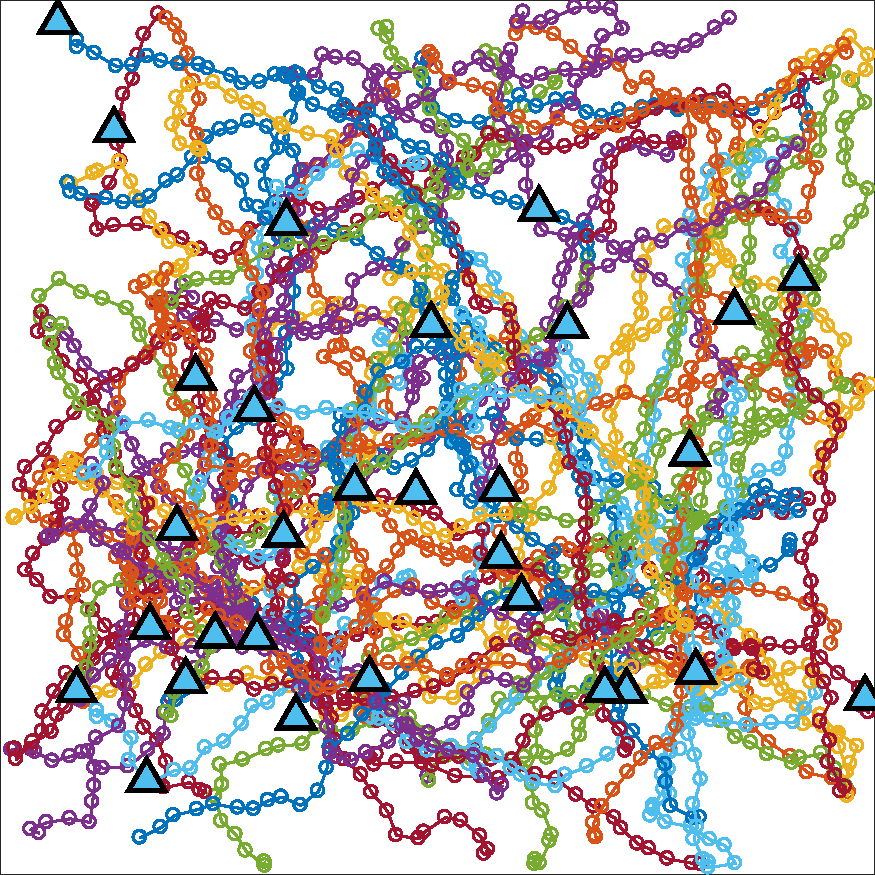
\includegraphics[width=50mm]{pics/synthetic_raw.pdf}&
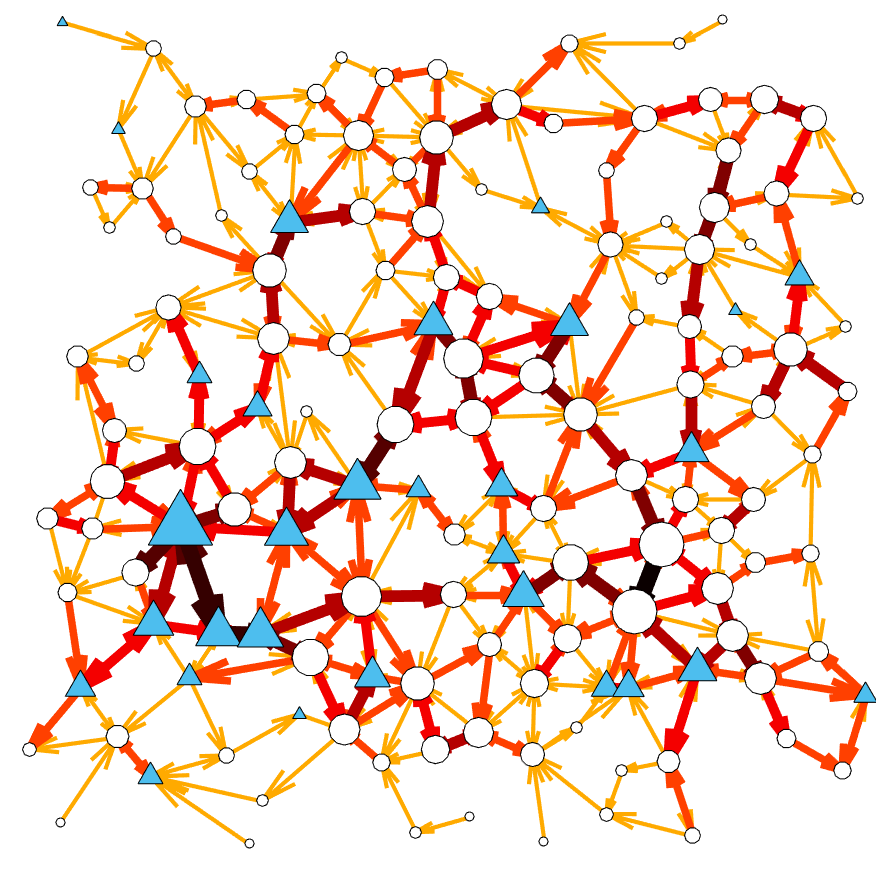
\includegraphics[width=50mm]{pics/syn_with_visualization.pdf}&
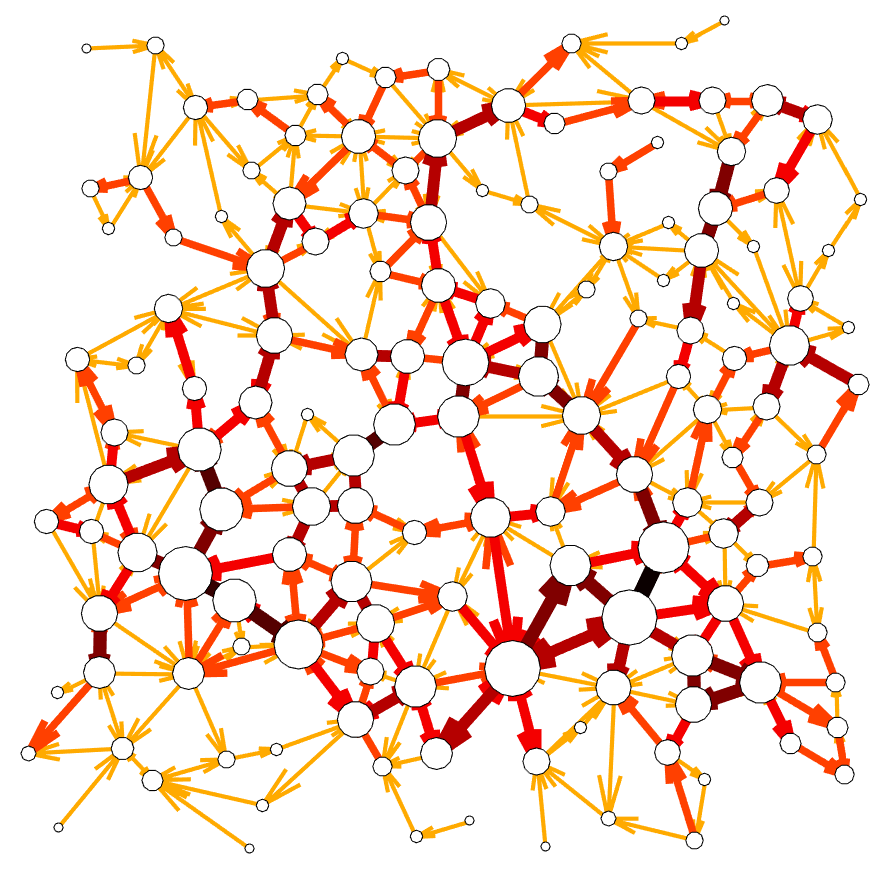
\includegraphics[width=50mm]{pics/syn_without_visulization.pdf}\\
(a) 人工数据集 & (b) 包含语义ROI的网络 & (c) 不包含语义ROI的网络  \\
\end{tabular}
\caption{100条人工轨迹的语义压缩结果。(b)在其中一层取($\epsilon=5$米)的压缩结果,随机取了30个点作为语义ROI。(c)在相同参数下没有选取语义ROI的结果。}
\label{fig:syntheticData} 
\end{figure}

\smallsection{真实数据集} 
我们在著名的四个真实数据集上实现我们的算法: Geolife, T-drive, Hurricanes\footnote{\url{http://www.nhc.noaa.gov/data/hurdat/}}和Migration\footnote{\url{https://www.datarepository.movebank.org/handle/10255/move.655}}。其中Geolife是Zheng等人\citeup{zheng2008understanding,zheng2009mining,zheng2010geolife}从人们的真实出行数据中收集记录下来的。T-drive数据集是Yuan等人\citeup{yuan2010t,yuan2011driving}从Uber司机出记录下的轨迹数据。Geolife和T-Drive都是北京市的数据集,其主要区别在于采样率, Geolife大约$91\%$的轨迹都很密集,两点之间间隔1-5秒或者5-10米,而T-Drive数据集的采样率就很低,大约2-5分钟才采样一个点。Hurricanes数据集记录了大西洋1851-2018年的数据,已经在图\ref{Hurricane_raw}中进行了可视化。Migration数据集记录了南美洲候鸟迁徙的轨迹。这四个数据集都是以经纬度和采样时间呈现的,统计数据见表\ref{tab:datasets}。



% \smallsection{语义信息的选取} 
为了在真实数据中生成语义信息,我们从OpenStreetMap\footnote{\url{https://www.openstreetmap.org}}下载了北京的城市路线图。路线图由节点和边缘表示。我们随机选择1000个交叉点,即度数大于2的节点,作为T-Drive和Geolife数据集上的固定语义ROI。 这里我们不介绍飓风和迁移数据的语义ROI,因为在在这两个数据集中定义语义点或区域是没有意义的。

\smallsection{评判指标} 
通常,传统的轨迹压缩算法通过压缩比来评估,其定义如下。
\begin{equation}
\text{压缩率} = 1- \sum_i\frac{|T_i'|}{|T_i|} \times 100\%,
\label{eq:ratio}
\end{equation}
其中每个$T_i\in\mathcal{T}'$ 是原始轨迹集$\mathcal{T}'$的一条轨迹,$T'_i$是其压缩后的结果。$|T_i|$表示轨迹$T_i$的点数或区域数。 然而,由于在压缩率和语义信息保存之间存在折衷,因此该度量不能完全评估我们模型的性能。 为了测量语义信息的持久性,我们还计算了误差$\eta$,它定义为真实点$p$与其压缩点$p'$之间的距离。在这里可以记录所有点的平均值和标准偏差。此外,我们还比较了四个真实世界数据集上所有算法的运行时间。


\tabcolsep=1pt
\begin{table}[!bt]\renewcommand{\arraystretch}{1.3}
\caption{四个真实数据集的统计信息。}
\center
% \scriptsize
\begin{tabular}{lcccc}
\hlinew{1pt} \textbf{数据集}& \textbf{点数}& \textbf{轨迹数}& \textbf{经纬度范围} & \textbf{[宽 $\times$ 高](米)}\\ \hlinew{1pt}
\textbf{Geolife}
& 24,876,978 & 18,670 & $[116.194, 116.553, 39.751, 40.033]$ & $[31024\times 31368]$ \\
\textbf{T-Drive}
& 6,969,481 & 8,768 & $[116.194, 116.553, 39.751, 40.033]$ & $[31024\times 31368]$ \\
\textbf{Hurricane}
% & 49,682 & 1,830 & $[-113.708, 44.713, 5.221,  74.725]$ & $[7,728,525\times 10,860,114]$ \\
& 49,682 & 1,830 & $[-113.708, 44.713, 5.221,  74.725]$ & $[7.728 \times 10.860]\times10^6 $ \\
\textbf{Migration}
% & 4,544 & 9 & $[-69.746, -33.8018, -39.605, 16.802]$ & $[6,272,361\times 3,915,386]$ \\
& 4,544 & 9 & $[-69.75, -33.80, -39.61, 16.80]$ & $[6.272\times 3.915]\times10^6$ \\
\hlinew{1pt}
\end{tabular}
\label{tab:datasets}
\end{table}


\tabcolsep=0pt
\begin{figure*}[!htb]
\centering
% \footnotesize
\begin{tabular}{cc}
{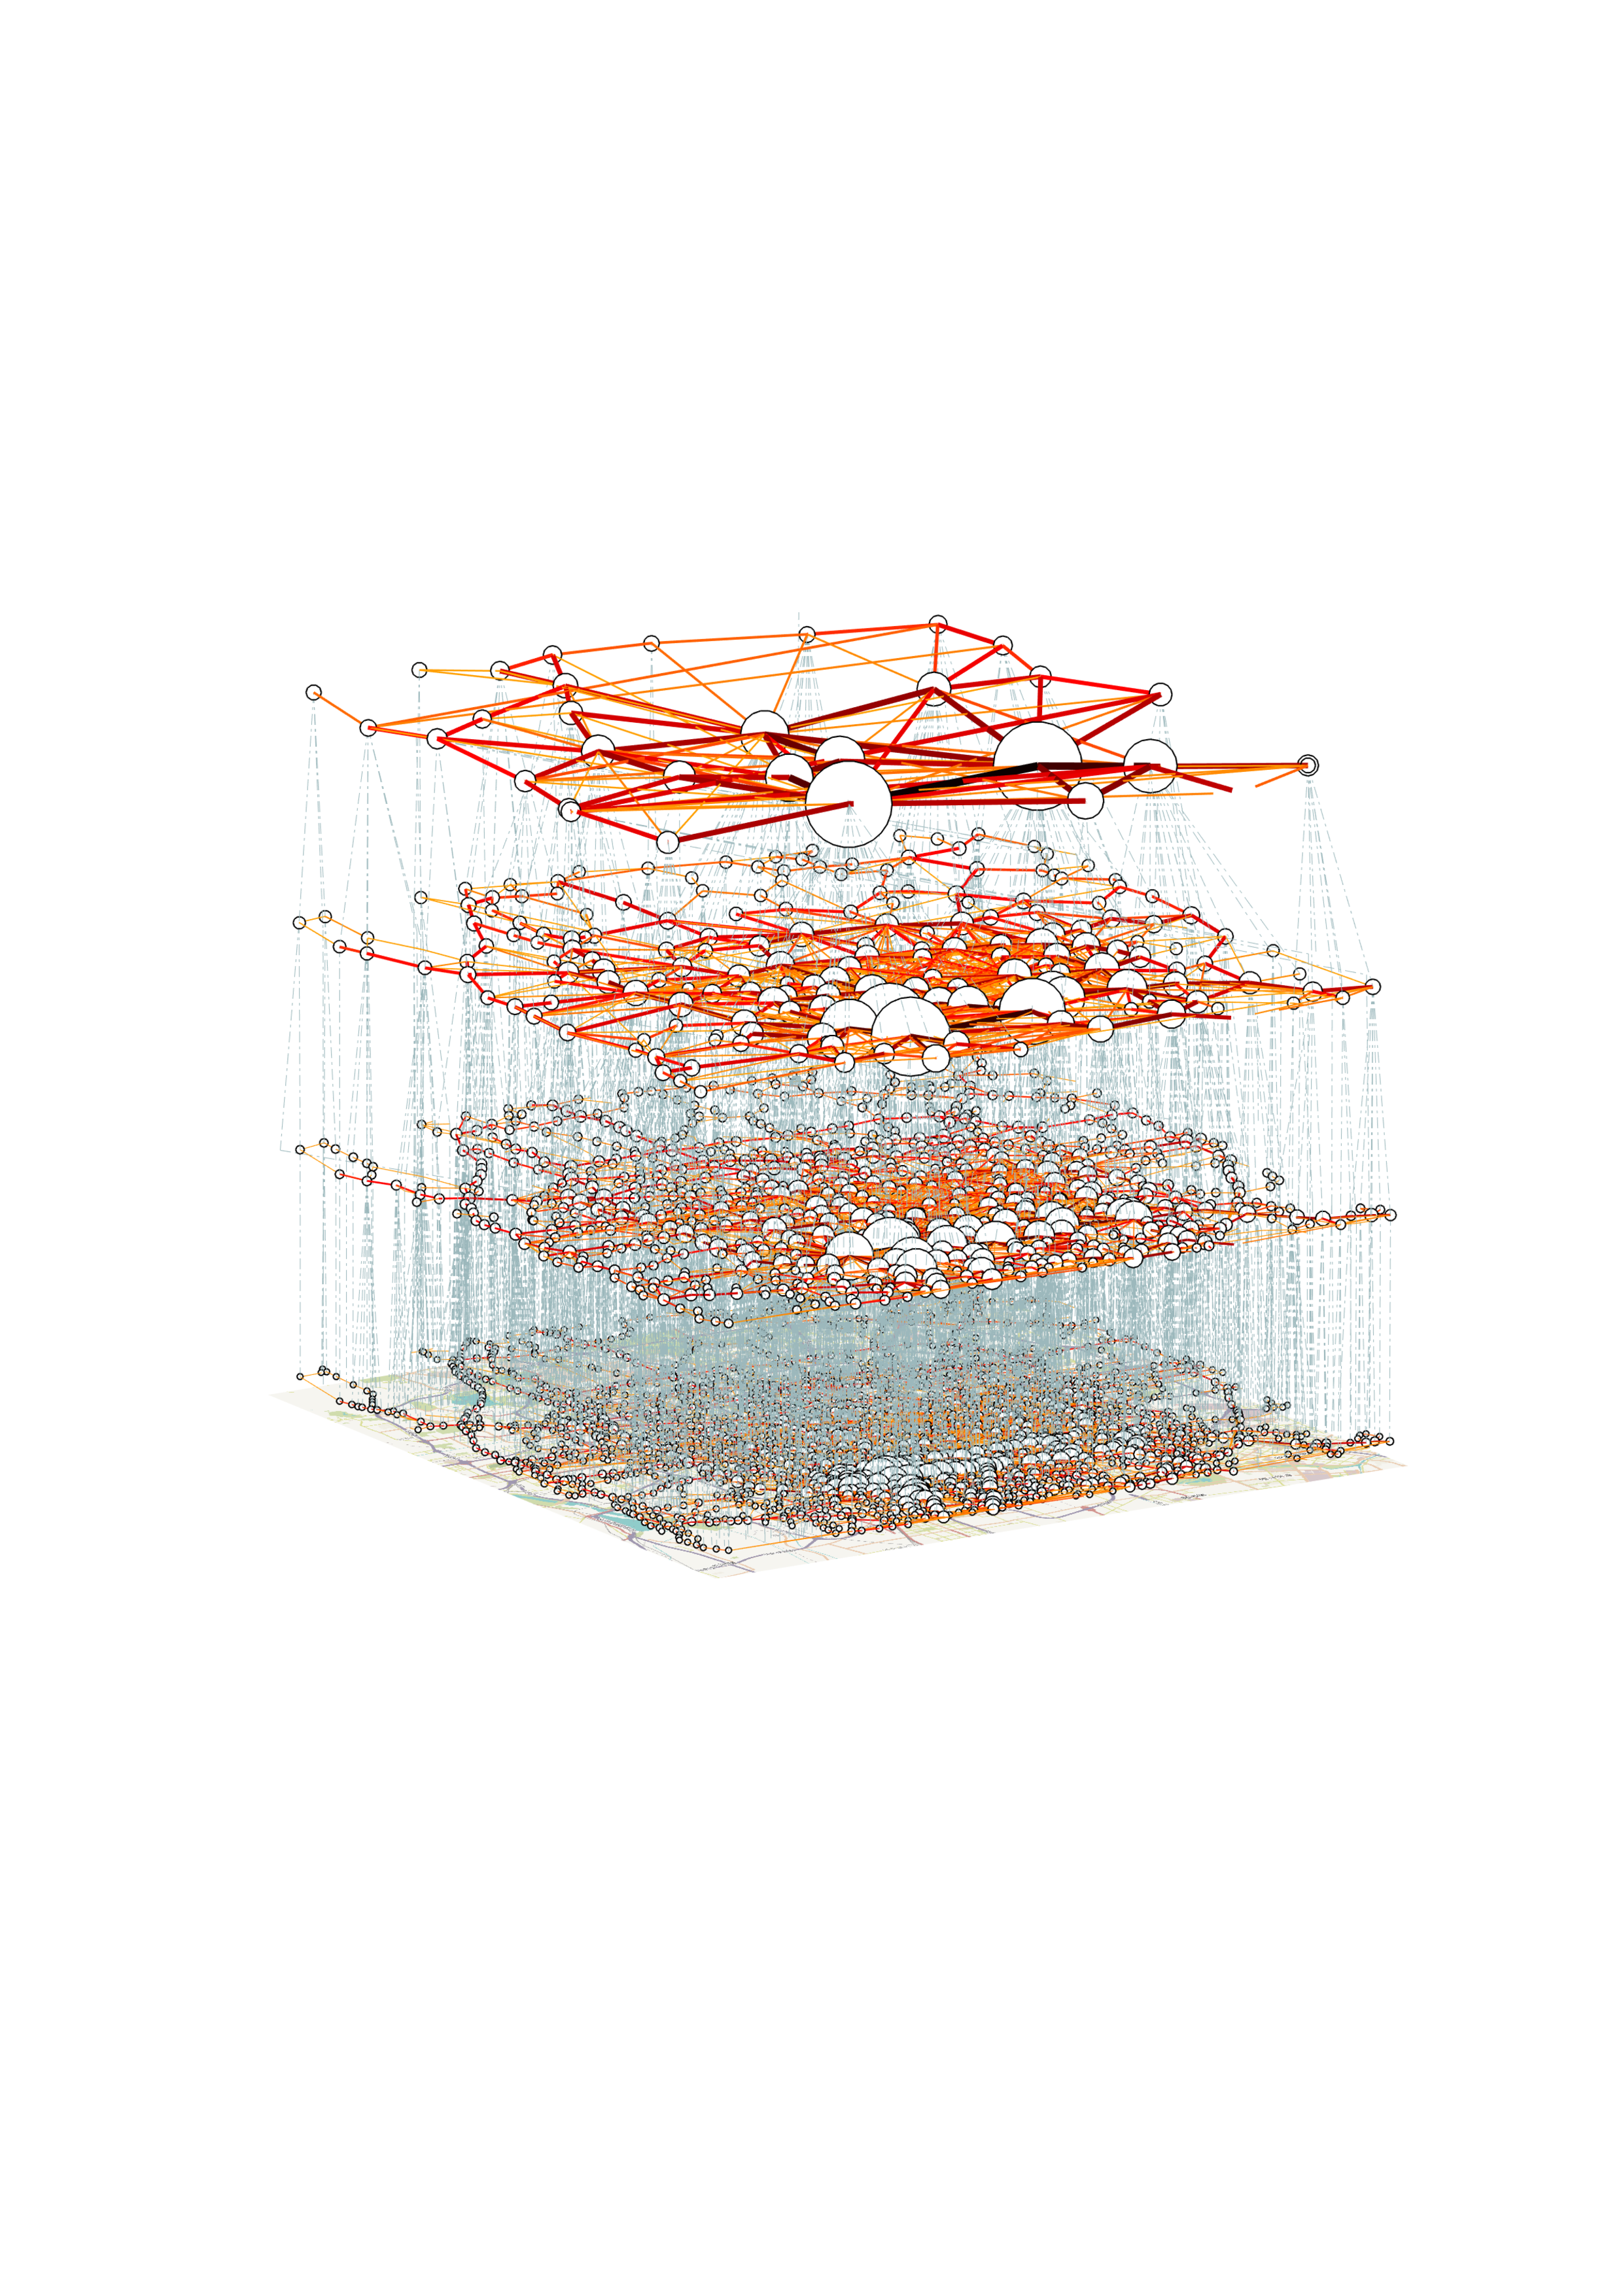
\includegraphics[width=84mm]{pics/withLine3.pdf}} & 
\begin{minipage}[b]{67mm}
\centering
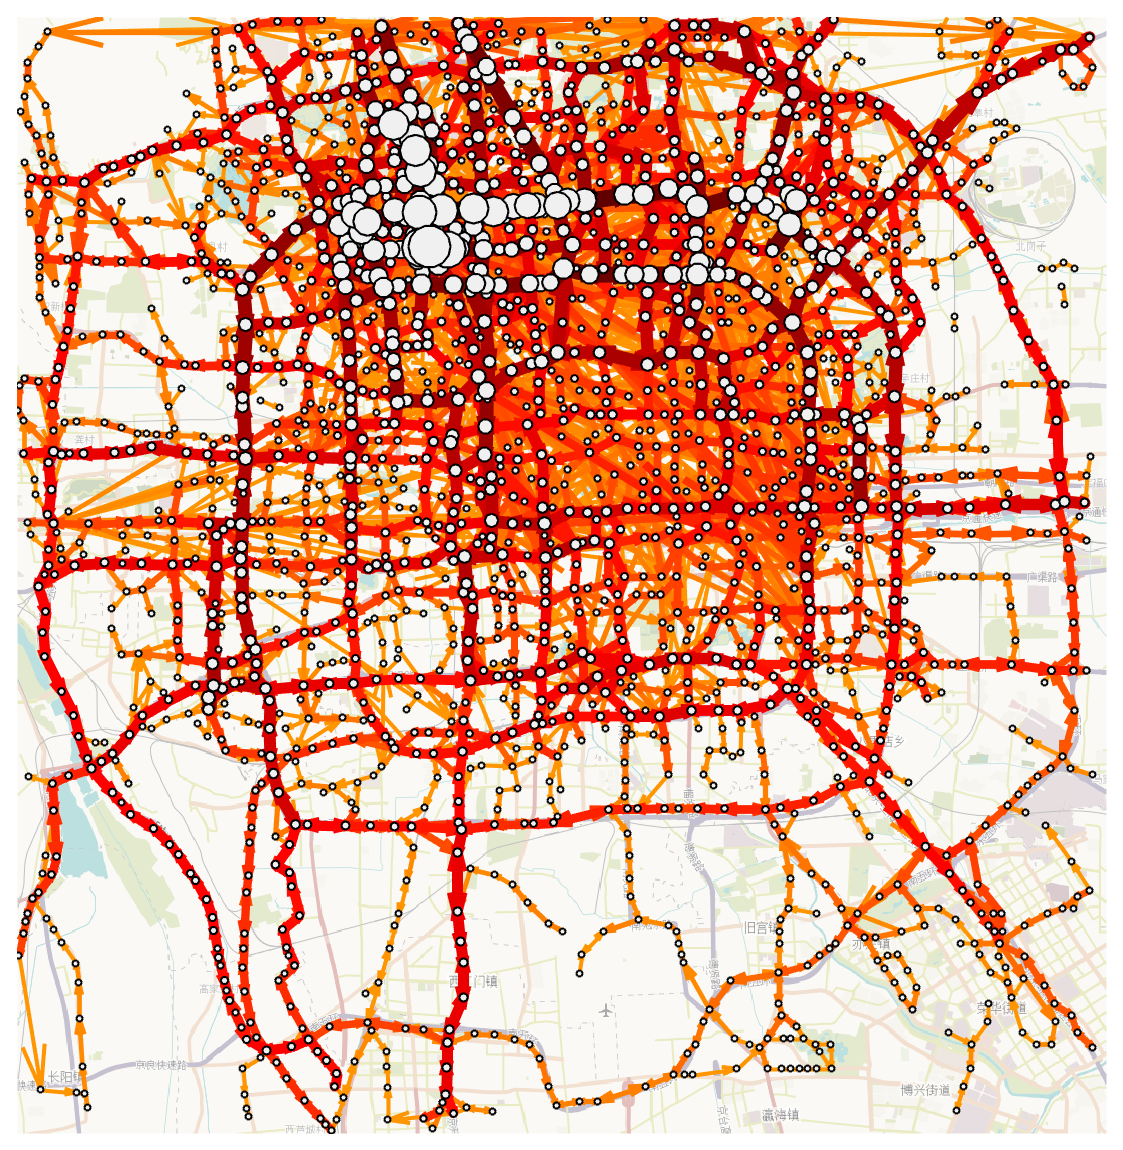
\includegraphics[width=32mm]{pics/geolife200m.eps}
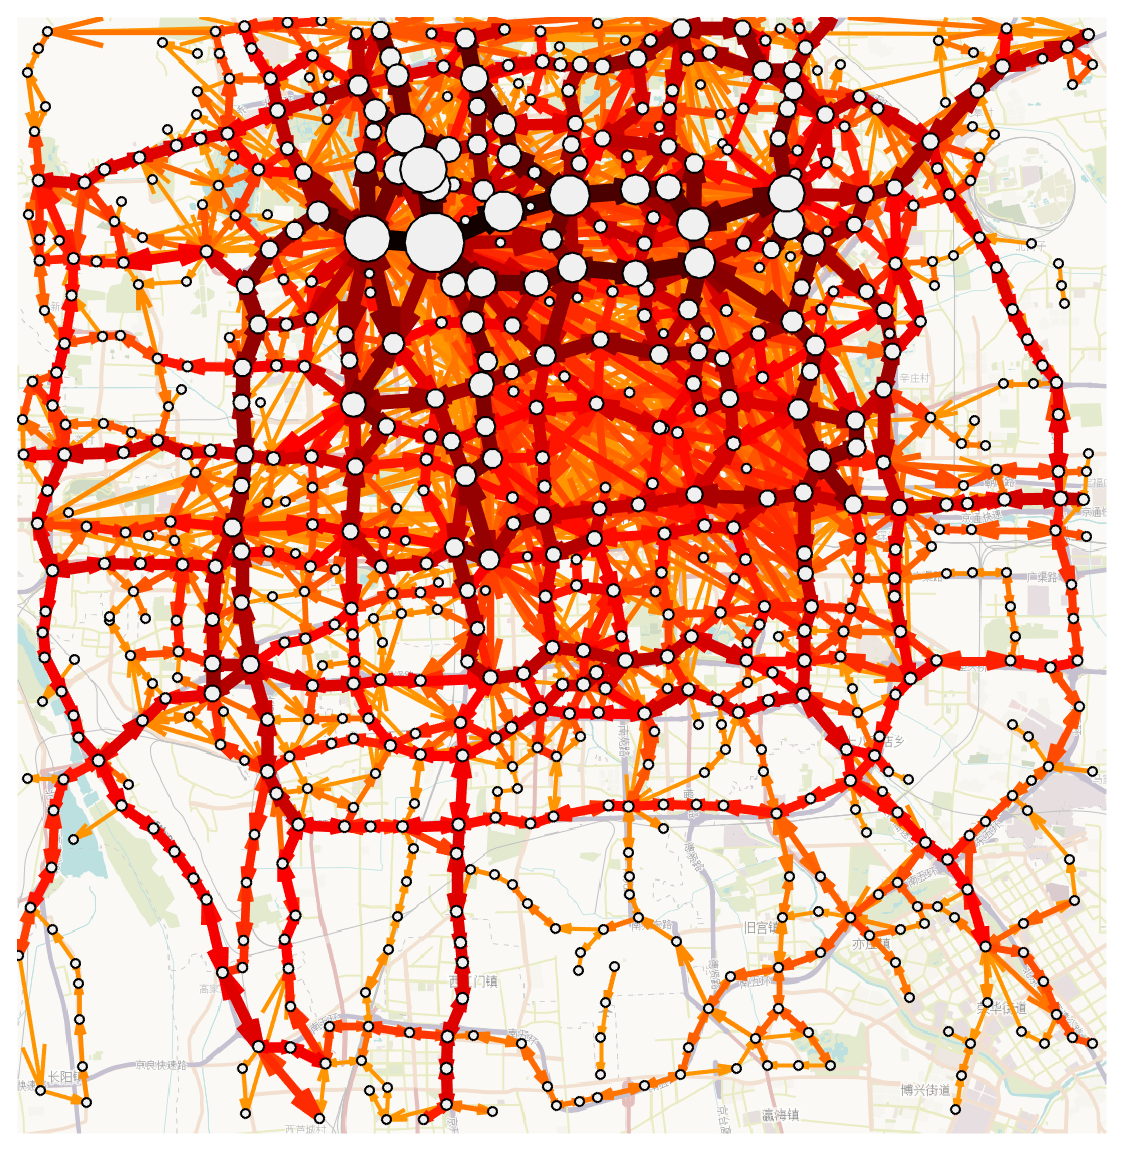
\includegraphics[width=32mm]{pics/geolife200_500m.eps}\\
(b) $\epsilon = 200$m  \hspace{5mm}(c) $\epsilon = 500$m\\
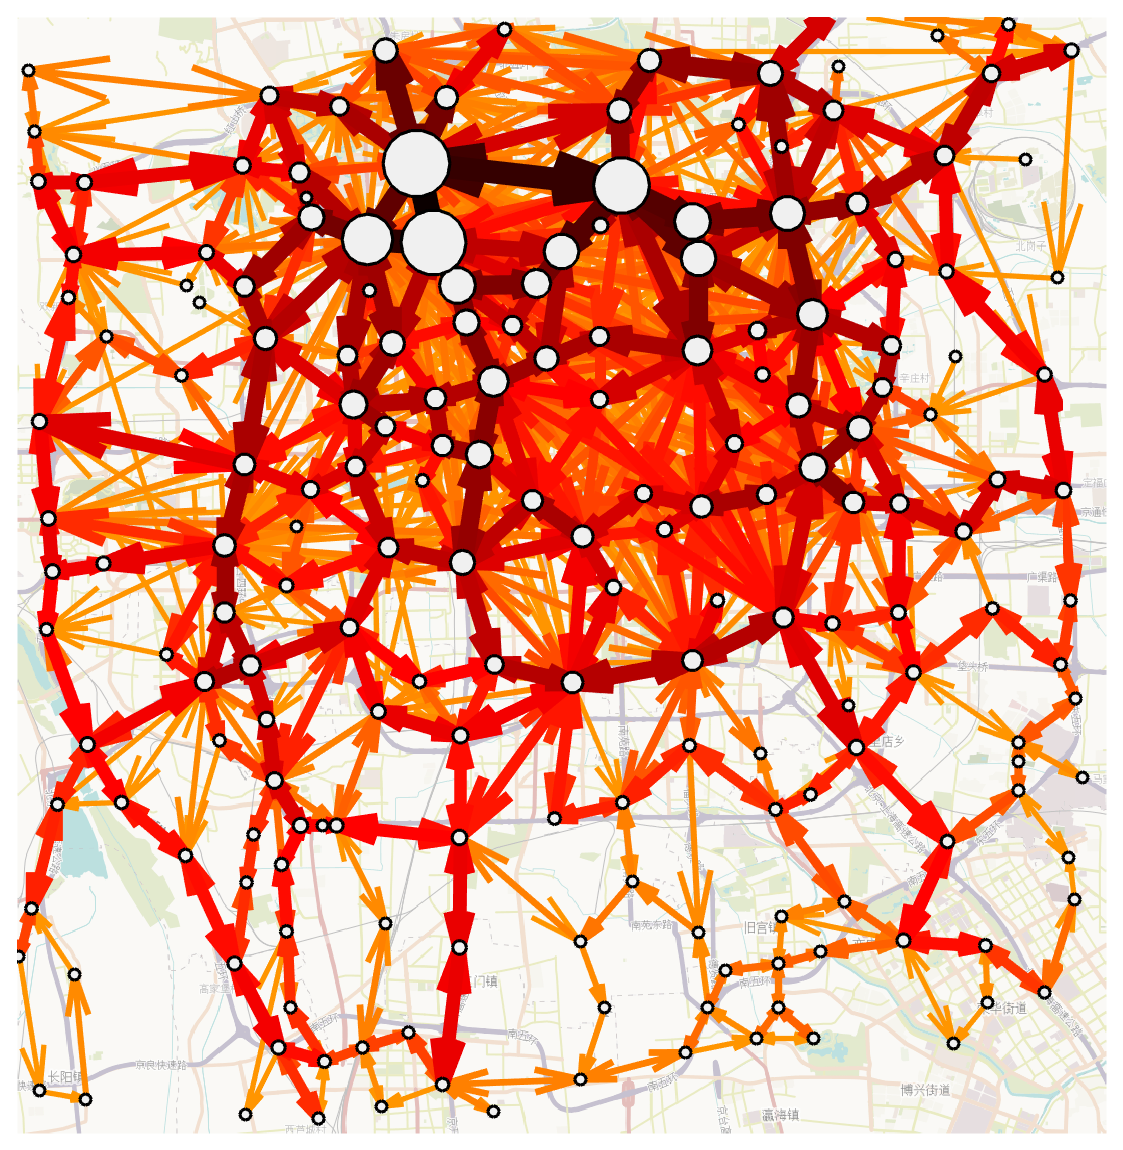
\includegraphics[width=32mm]{pics/geolife200_500_1000m.eps}
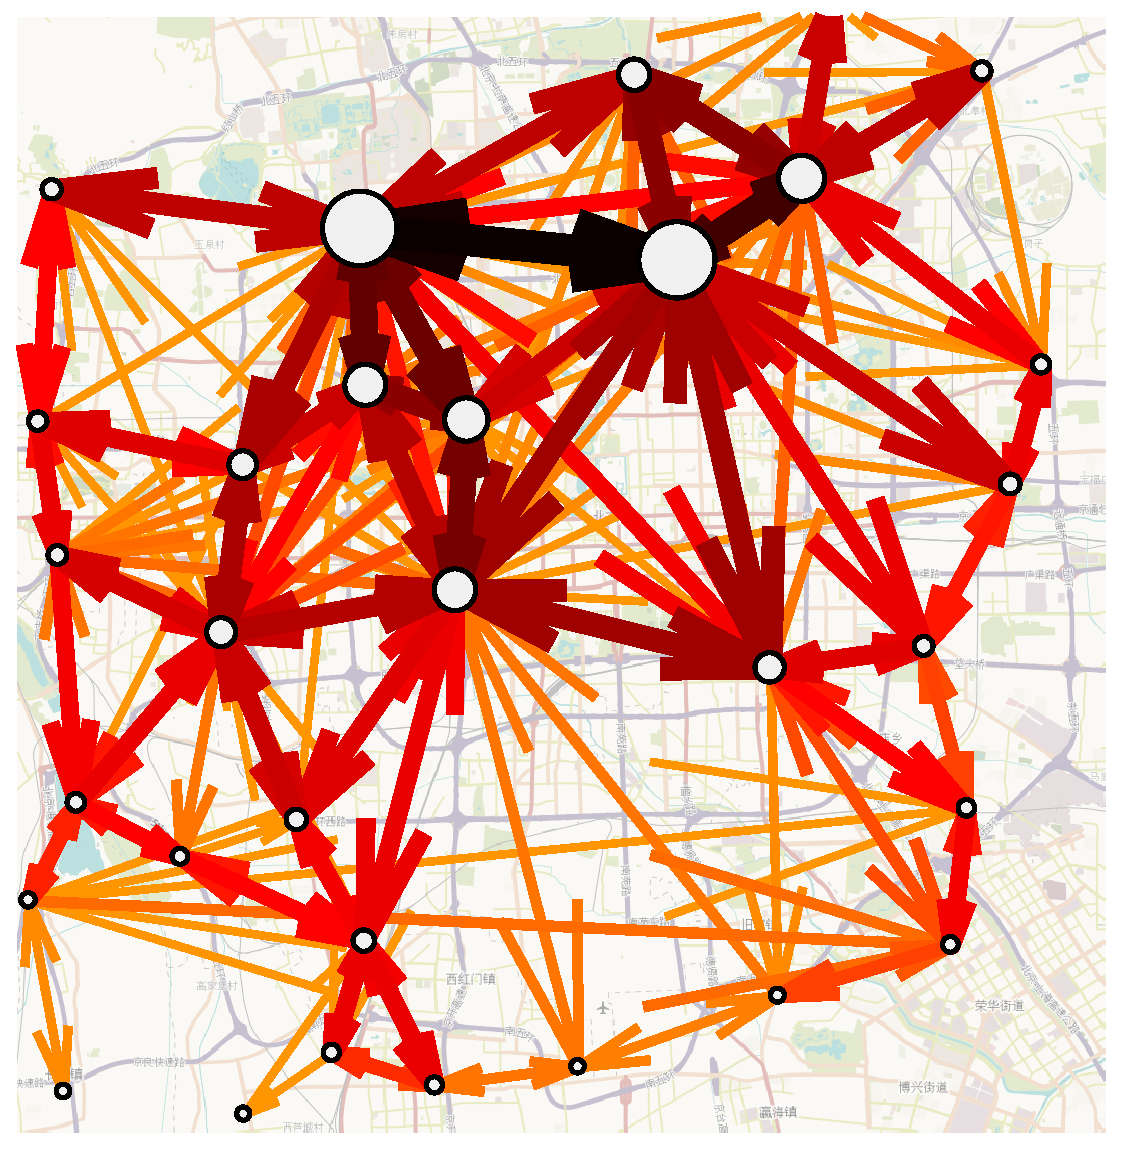
\includegraphics[width=32mm]{pics/geolife200_500_1000_3000m.eps}\\
\end{minipage}\\
(a) Geolife上的多层次ROI网络 & (d) $\epsilon = 1000$m  \hspace{5mm}(e) $\epsilon = 3000$m\\
\end{tabular}
\caption{在Geolife数据上的四层ROI网络。}
\label{fig:network}
\end{figure*}


\smallsection{对比算法}
由于在包含语义约束的数据中,轨迹压缩方法的性能不便于直接比较,我们为了证明\CascadeSync的有效性和高效性,使用五种主流的的轨迹压缩算法在特定实验上进行比较。
\emph{Douglas-Peucker} \citeup{douglas1973algorithms}: 是最有名的线简化算法,它使用贪婪策略检查第一个和最后一个点之间的所有点,直到最大空间偏差在误差范围$\zeta$内。算法复杂度为$\mathcal{O}(n^2)$。

\emph{Douglas-Peucker-SED} \citeup{meratnia2004spatiotemporal,potamias2006sampling}:是原算法的改版。其充分考虑了移动物体的时空特性,将原始的垂直距离度量换位了同步欧式距离(Synchronized Euclidean Distance, SED)。最坏的时间复杂度为$\mathcal{O}(n^2)$。

\emph{Dead Reckoning} \citeup{trajcevski2006line,muckell2011squish}:它是一种在线压缩模型。原理是通过当前位置和速度估算每个后继位置。通过计算估计位移和真实位置之间的偏差,如果偏差小于误差界限,则可以将点保持在压缩轨迹之外。时间复杂性是$\mathcal{O}(n)$。

\emph{Squish} \citeup{muckell2011squish,muckell2014compression}:使用了一个优先级队列,其中每个点的优先级被定义为若将该点的移除带来的误差。SQUISH通过从优先级队列中删除最低优先级的点来压缩每一条轨迹,直到达到目标压缩比或误差界限。Squish的时间复杂度为
$\mathcal{O}(\log n)$。

\emph{Traclus-MDL} \citeup{lee2007trajectory}:是一种固定压缩率的算法,其用最小描述长度(MDL)\citeup{grunwald2005advances} 来综合地描述模型的复杂度和表征能力,然后输出最平衡的一个压缩结果。其时间复杂度为$\mathcal{O}(n)$。

我们可以在给定误差范围的情况下与这些基线算法进行比较压缩比。此外,也可列出所有模型的压缩时间以比较效率。此外,我们还说明了\CascadeSync中语义ROI带来的影响。

\pic[!htb]{带语义ROI的Geolife上的多层次ROI网络。}{width=125mm}{with}

\subsection{实验结果与分析}
% \subsection{基本性质的证明}
\smallsection{ROI网络可视化}
为了说明,我们首先可视化ROI网络。为了简洁起见,我们只能看到图\ref{fig:network}和图\ref{with}中的Geolife数据集上的多层ROI网络,它们是使用和不使用1000个固定交叉点的结果。 此外,从这些数据中,我们可以看到我们的模型在可视化方面是有效的,这可能为许多现实挖掘分析场景提供了基础。


\smallsection{表征误差分析}
与独立压缩每个轨迹的传统方法不同,我们基于同步的聚类模型 \CascadeSync将全局地压缩轨迹,并且代表性错误可以以很高地概率满足由$\zeta$的约束。我们将探索误差约束$\zeta$和交互范围$\epsilon$之间的关系。

在不失一般性的情况下,我们在Geolife数据集上进行此实验。24,876,978个 GPS点将被\Cascade表征为不同层次的ROI网络。我们将交互范围$\epsilon$从200米到2000米均匀地选择十次,大约是地图长度的$6/1000$到$60/1000$。通过增加模型中每层的交互范围,可以在不同级别的交互范围下计算所有点的平均代表性误差。其结果如图\ref{fig:relation}中的框图所示。框中的水平红线是中值,则蓝框的上边界是第三个四分位数,黑色虚线的上端表示最大值,超出最大值的红线被视为异常值。

没有预定义语义ROI的实验结果如图\ref{fig:relation}(a)所示,我们可以观察到误差最大值与交互范围$\epsilon$成正比,并且近似等于$\epsilon$。实际上,有$97.64\%$的点的表征误差小于$\epsilon$。换句话说,如果我们设置误差界为$\zeta=\epsilon$,没有语义ROI的\CascadeSync的结果将被$\zeta$以大于$0.9764$的概率约束住。

通过引入道路交叉点作为固定语义ROI,结果如图\ref{fig:relation}(b)。与之前不同,表征误差将先随着交互范围$\epsilon$的增加而增加,直到$\epsilon$达到$800$米,然后$\epsilon$继续增加而误差将保持不变。 在这个实验中,如果我们设置误差界为$ \zeta =\epsilon $,结果将以$ 0.9971 $的概率受$ \zeta $限制。

到目前为止,我们已经证明我们的方法\CascadeSync的误差将以非常高的概率被$ \zeta = \epsilon$所限制。此外,通过引入预定义的语义ROI,我们的模型还可以进一步减少表征误差。其原因很直观:更多的语义信息将会导致压缩结果中留有更多的语义ROI,但是,压缩比也会受到影响,我们将在下一个实验中展示。

\tabcolsep=3pt
\begin{figure}[!t]
\centering
% \footnotesize
% \vspace{-2mm}
\begin{tabular}{cc}
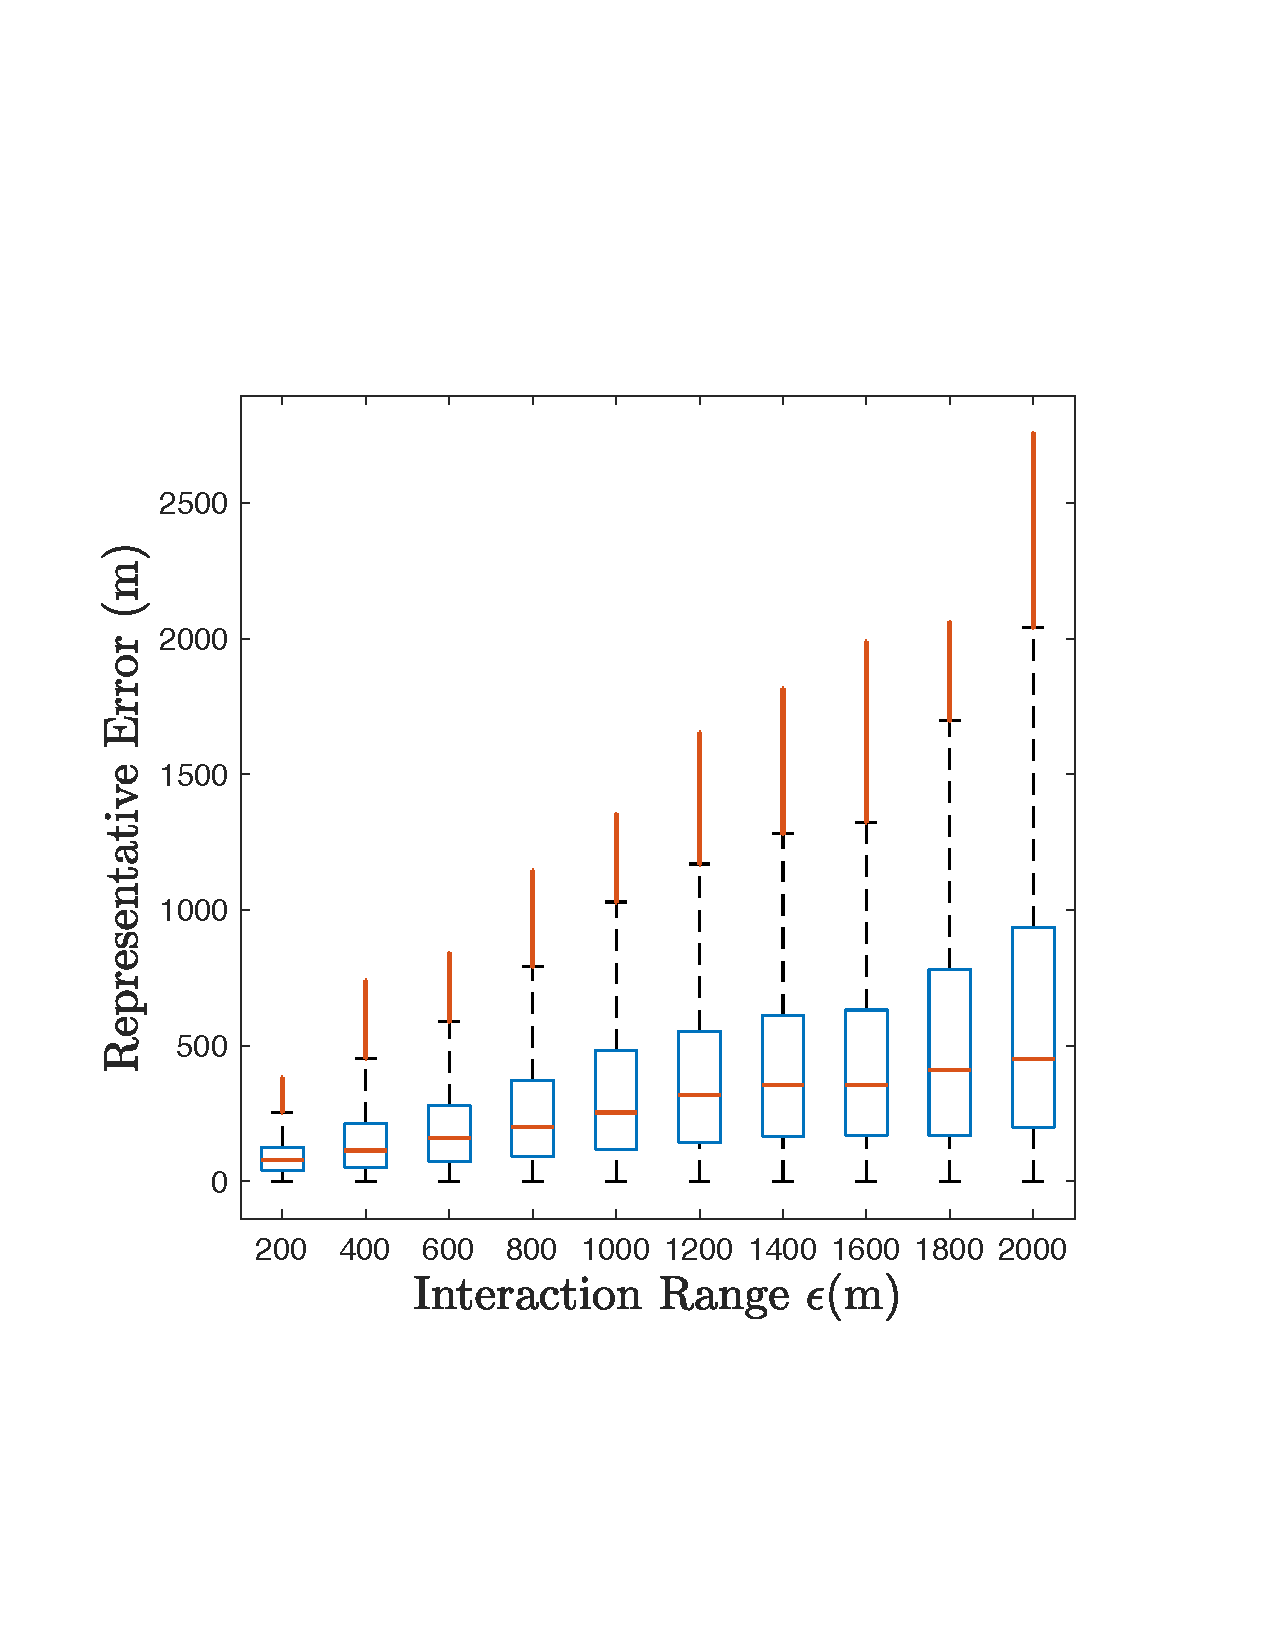
\includegraphics[width=70mm]{pics/relation_without2.pdf}&
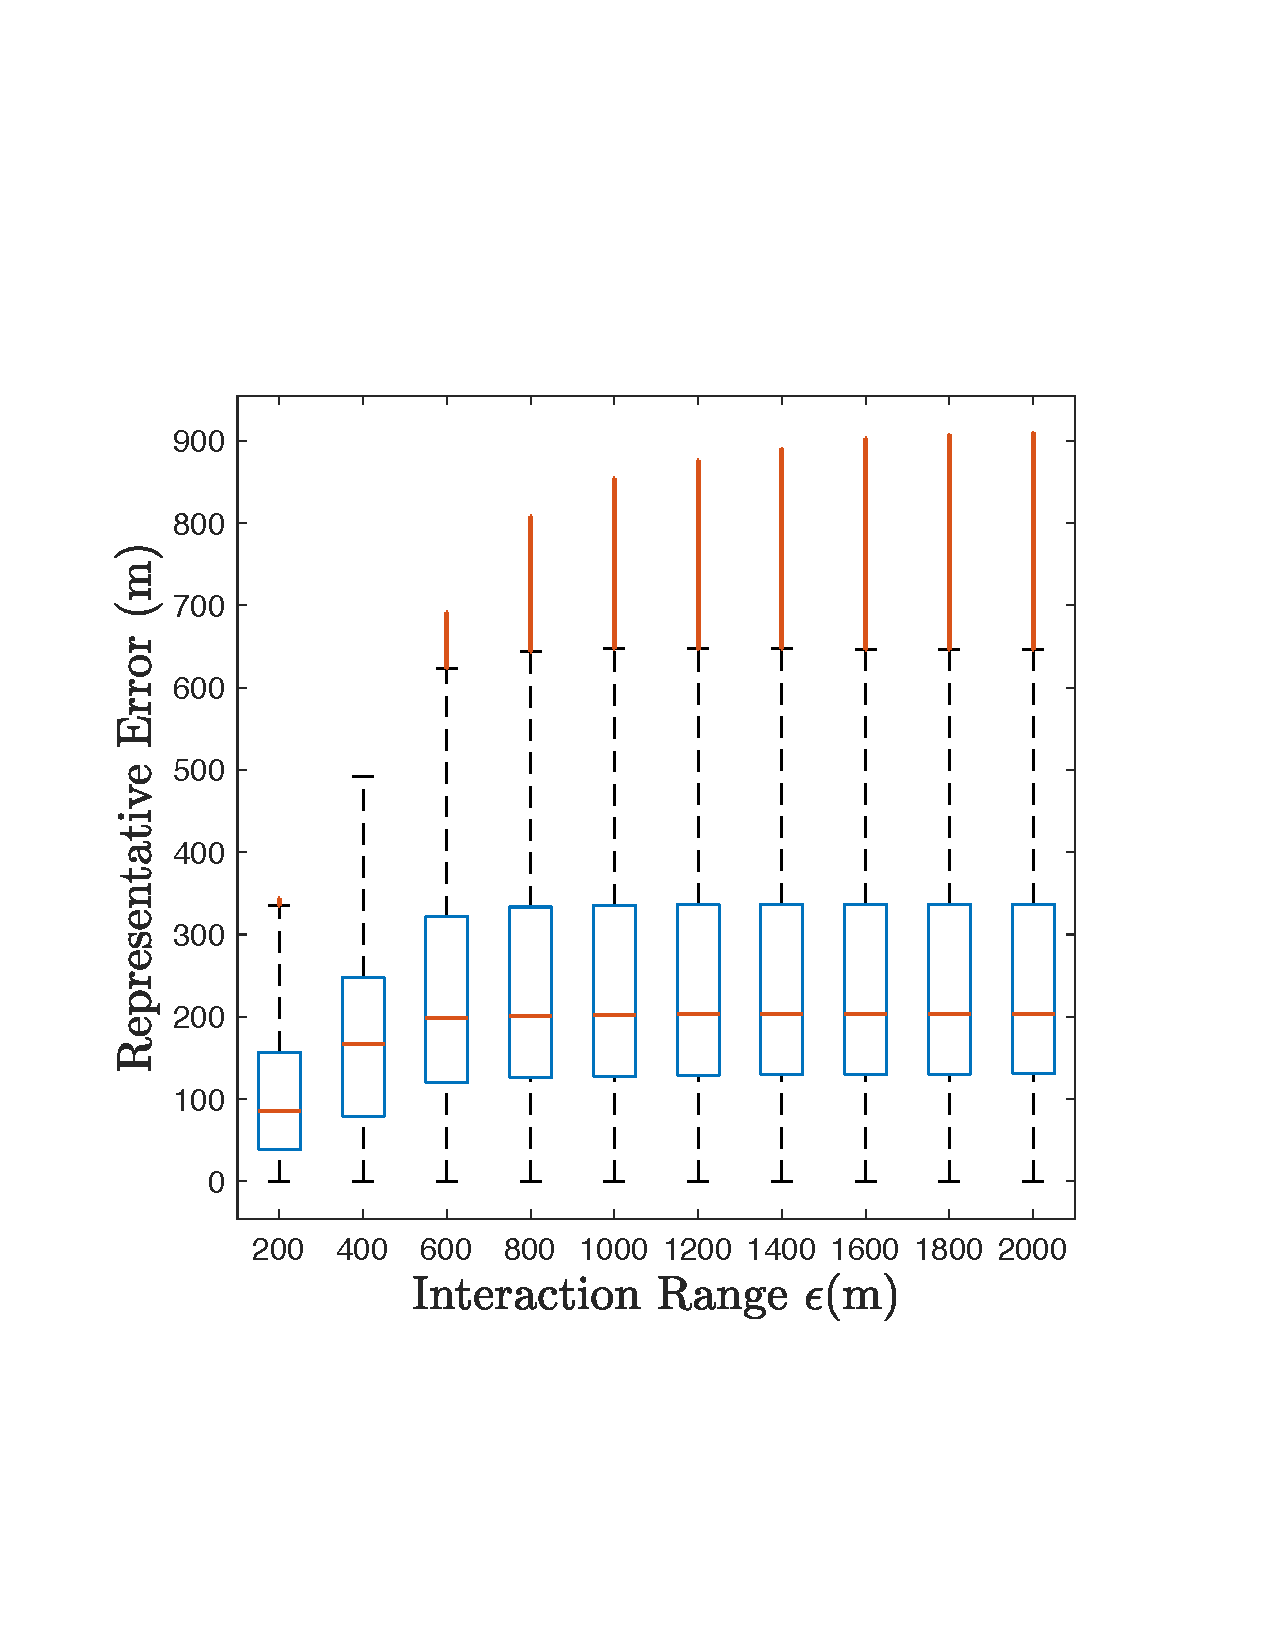
\includegraphics[width=68mm]{pics/relation_with2.pdf}\\
(a) 没有语义ROIs & (b) 有语义ROI \\
\end{tabular}
\caption{代表性误差与相互作用范围之间的关系。框中的水平红线是中值,蓝框的上边界是第三个四分位数,黑色虚线的上端表示最大值,超出最大值的红线被认为是异常值。}
\label{fig:relation}
\end{figure}



\tabcolsep=0pt
\begin{figure*}[!htb]
\centering
% \footnotesize
\begin{tabular}{ccccc}
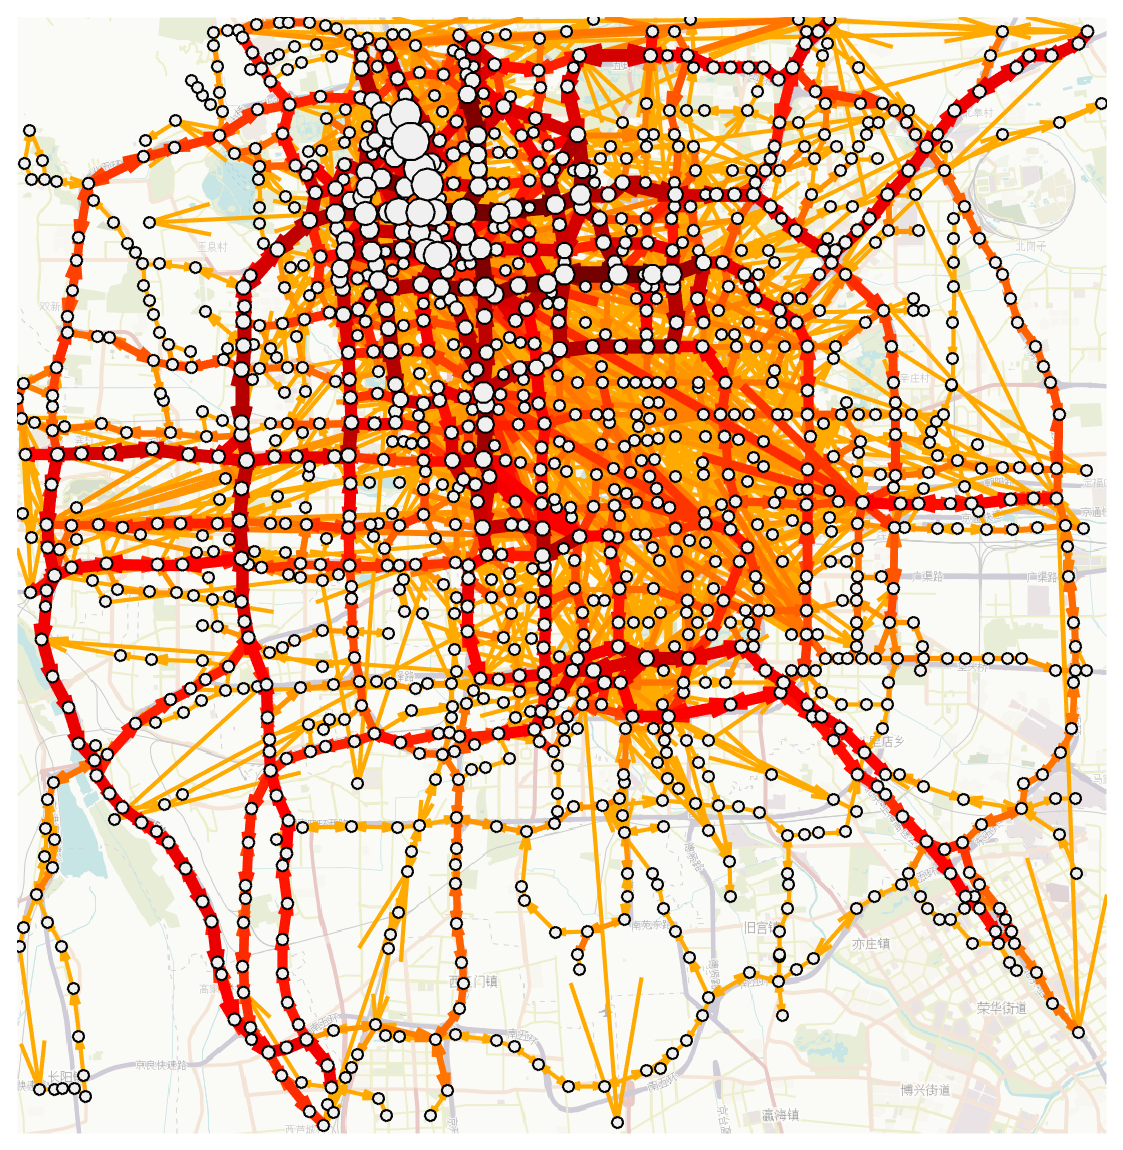
\includegraphics[width=35mm]{pics/Geolife200without.eps}&
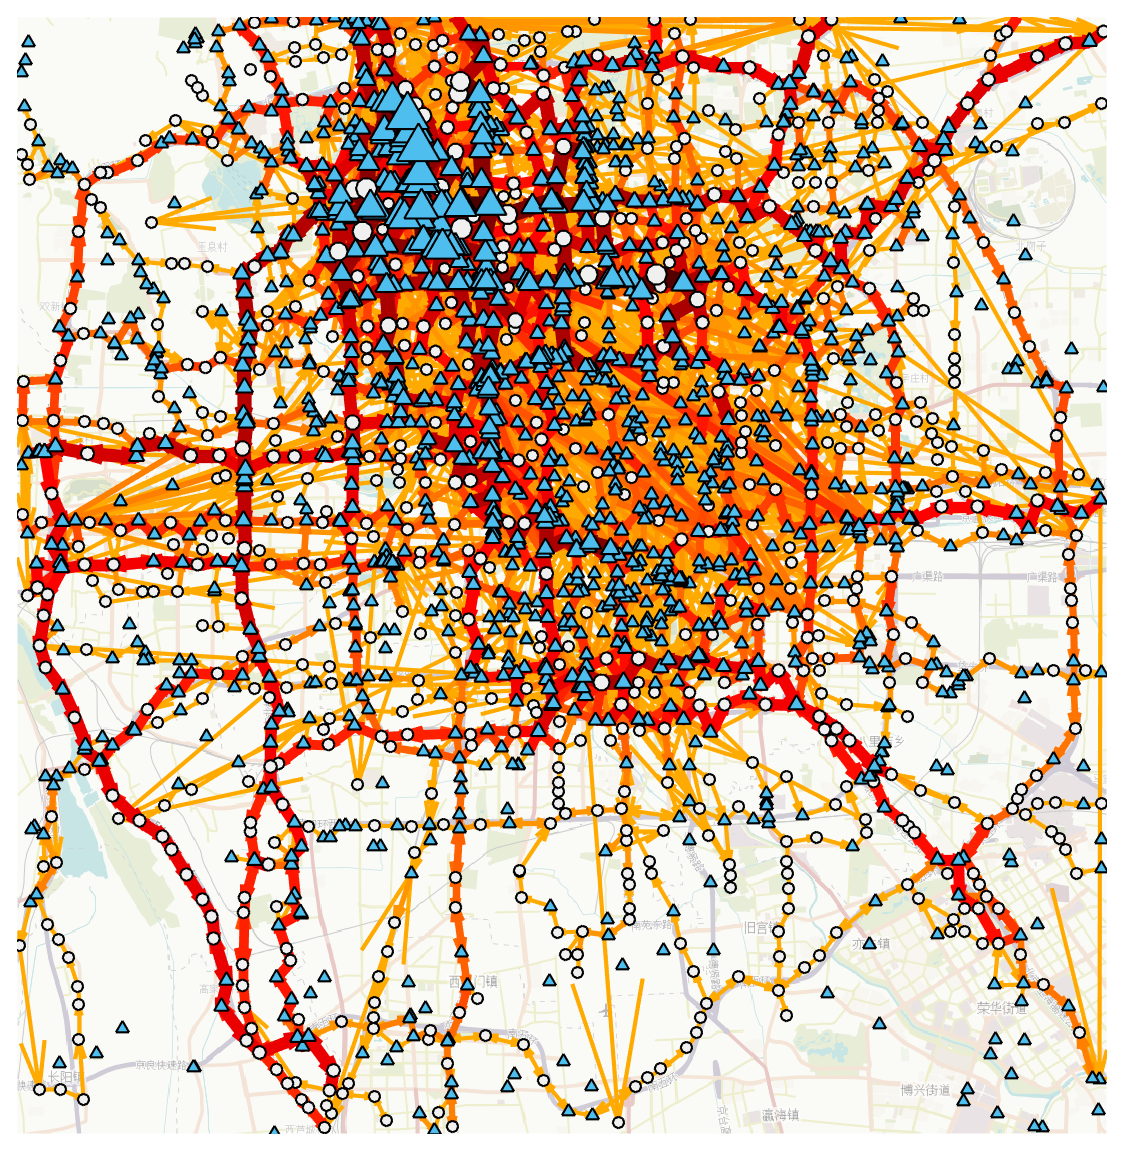
\includegraphics[width=35mm]{pics/Geolife200with.eps}&
~~&
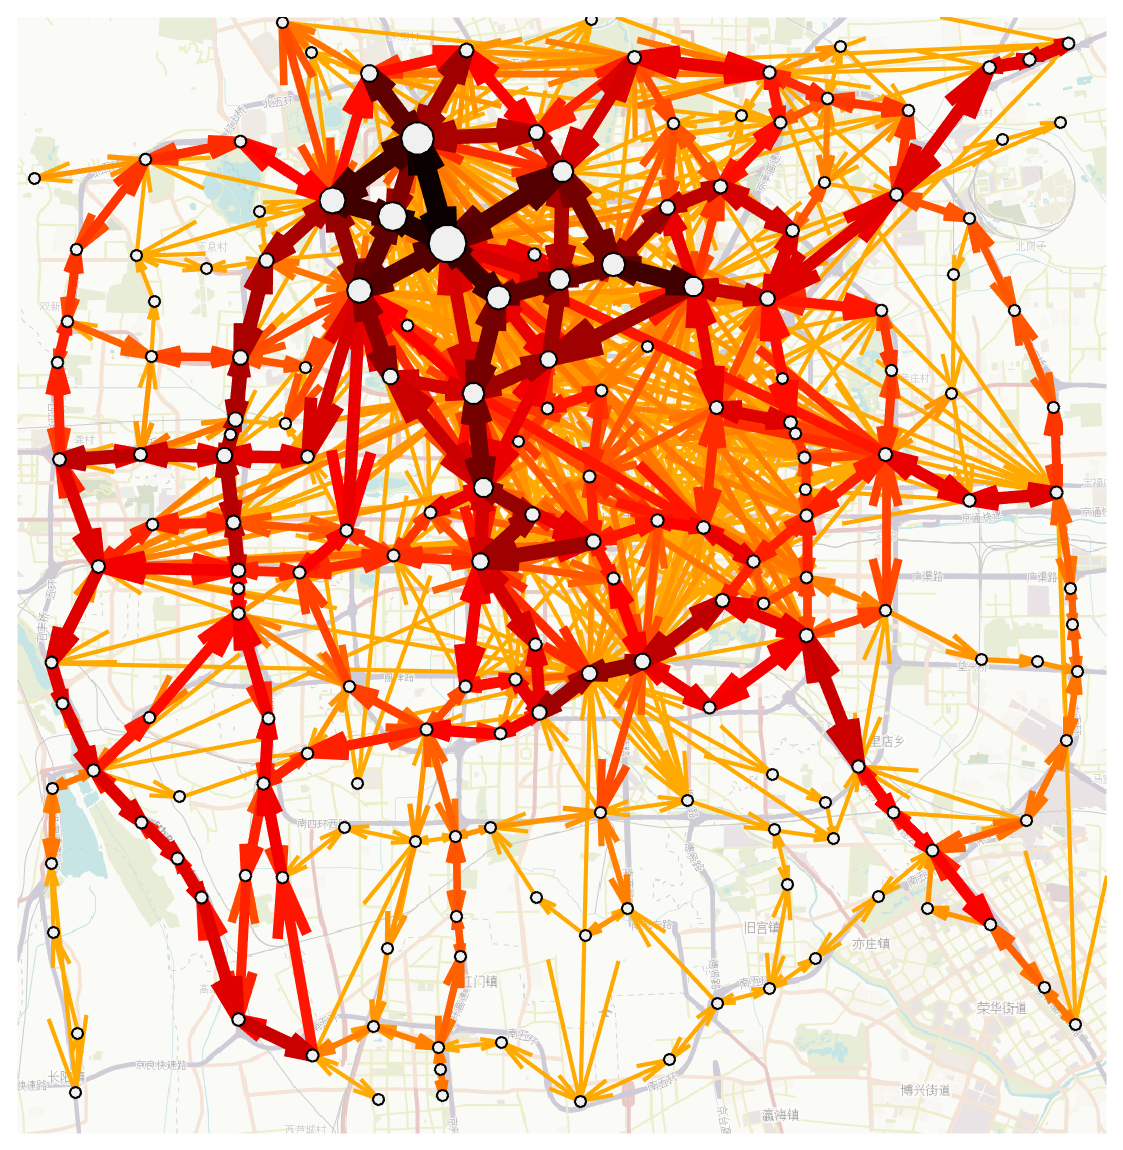
\includegraphics[width=35mm]{pics/Geolife1000without.eps}&
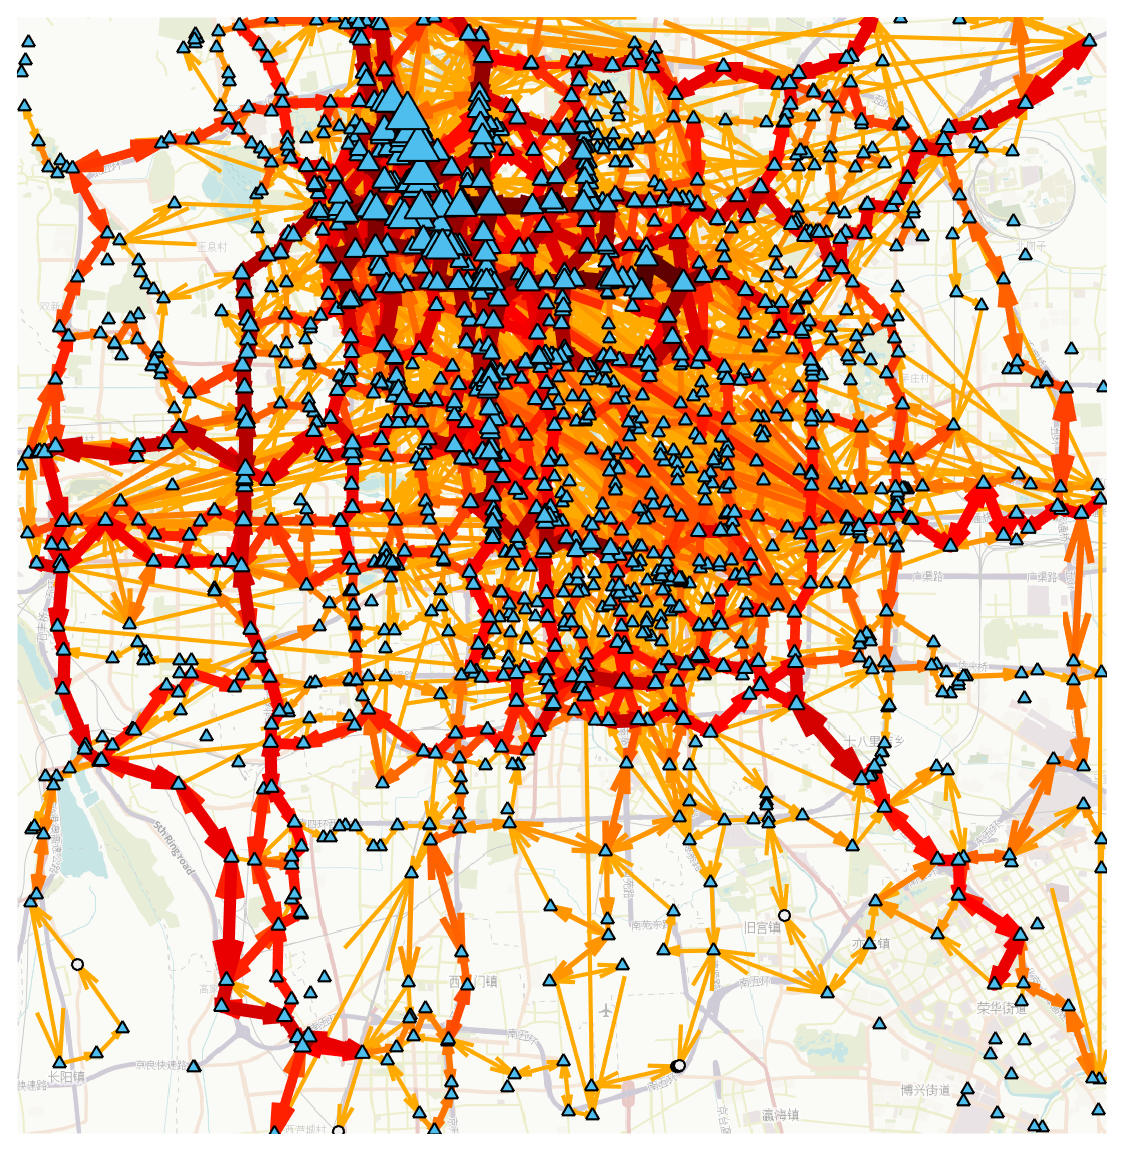
\includegraphics[width=35mm]{pics/Geolife1000with.eps}\\
% (a) Geolife: $\zeta = 200$m & (b) Geolife: $\zeta = 200$m & & (c) Geolife: $\zeta = 1000$m & (d) Geolife:$\zeta = 1000$m\\
\multicolumn{2}{c}{(a) Geolife: $\epsilon = 200$米} & & \multicolumn{2}{c}{(b) Geolife: $\epsilon = 1000$ (m)}\\
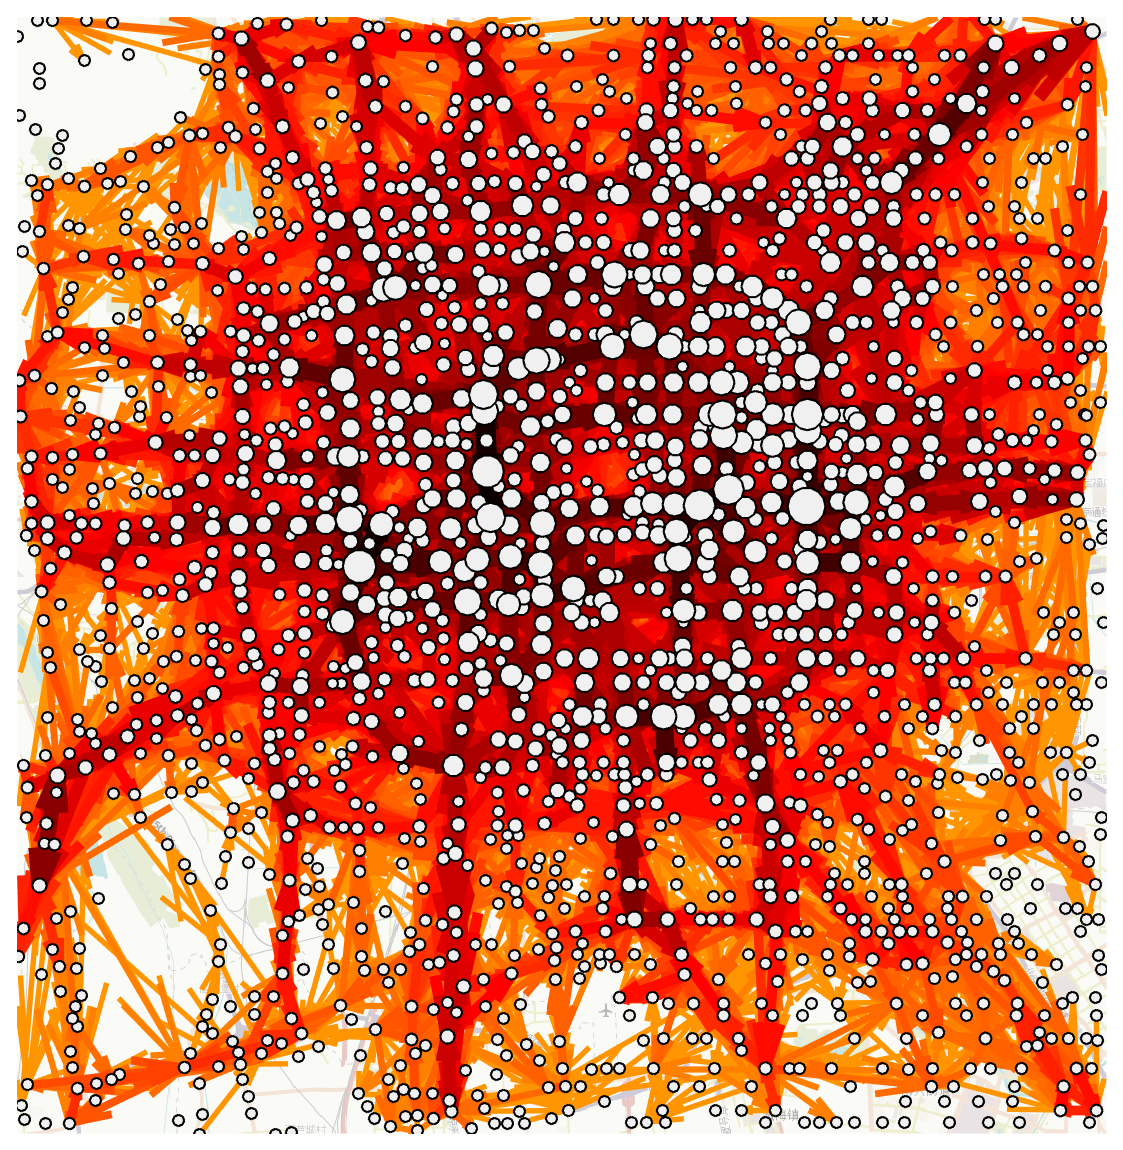
\includegraphics[width=35mm]{pics/tdrive200without.eps}&
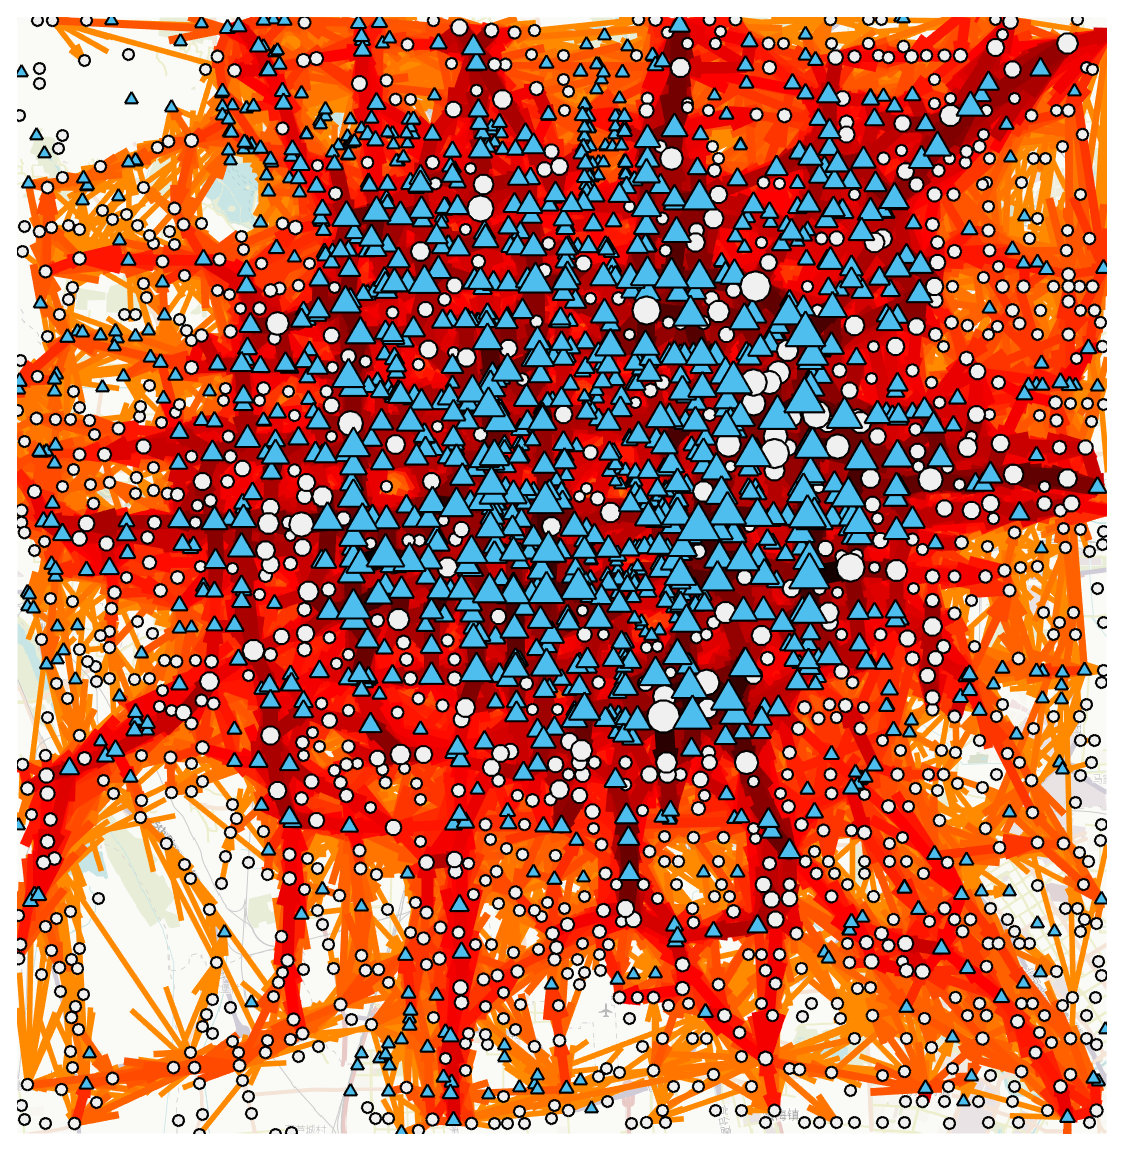
\includegraphics[width=35mm]{pics/tdrive200with.eps}&
~~&
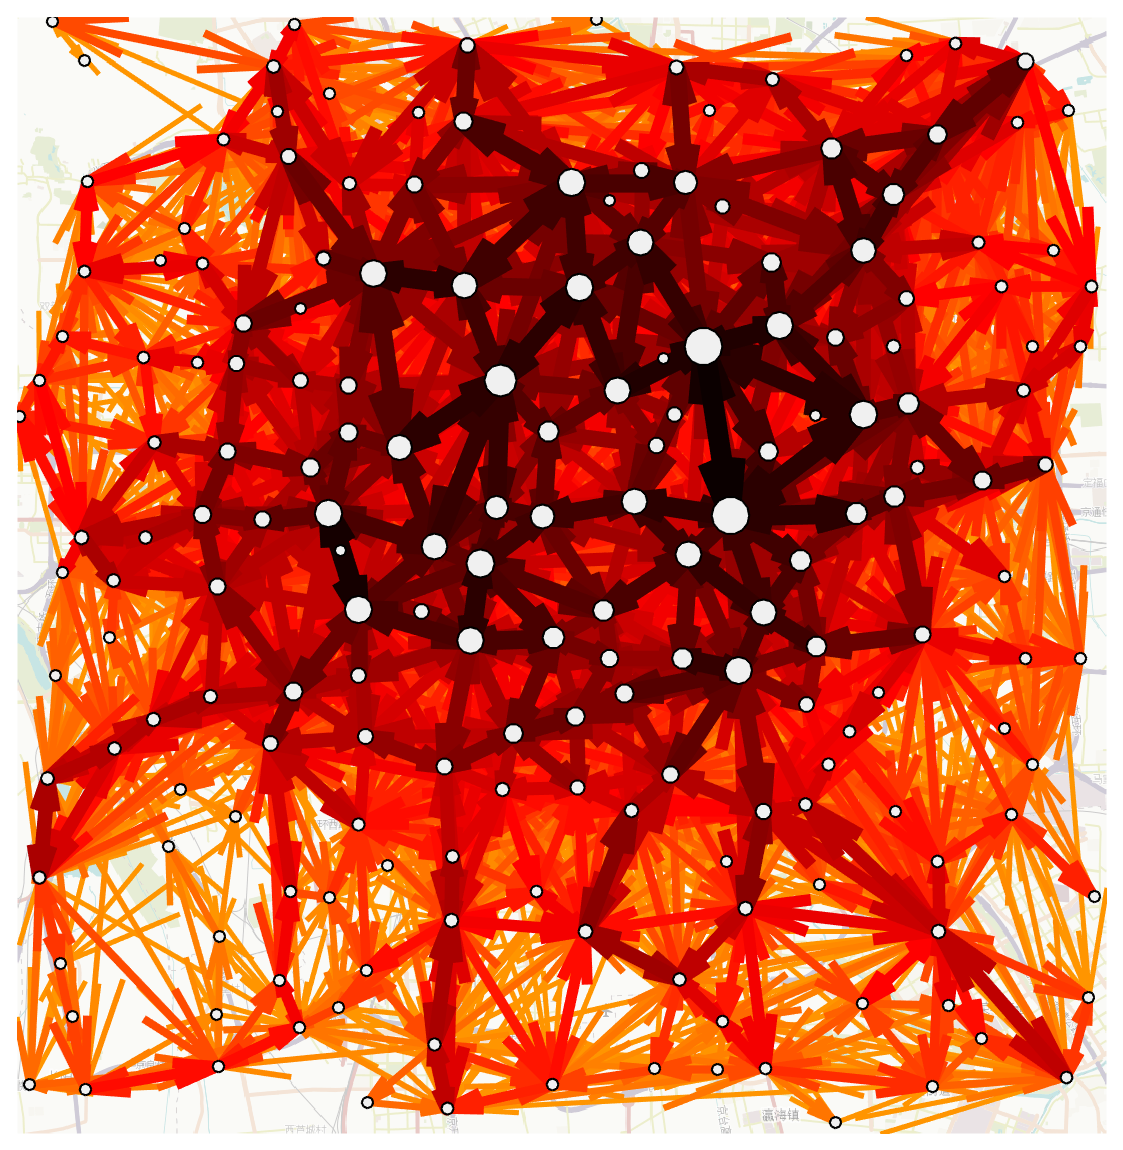
\includegraphics[width=35mm]{pics/tdrive1000without.eps}&
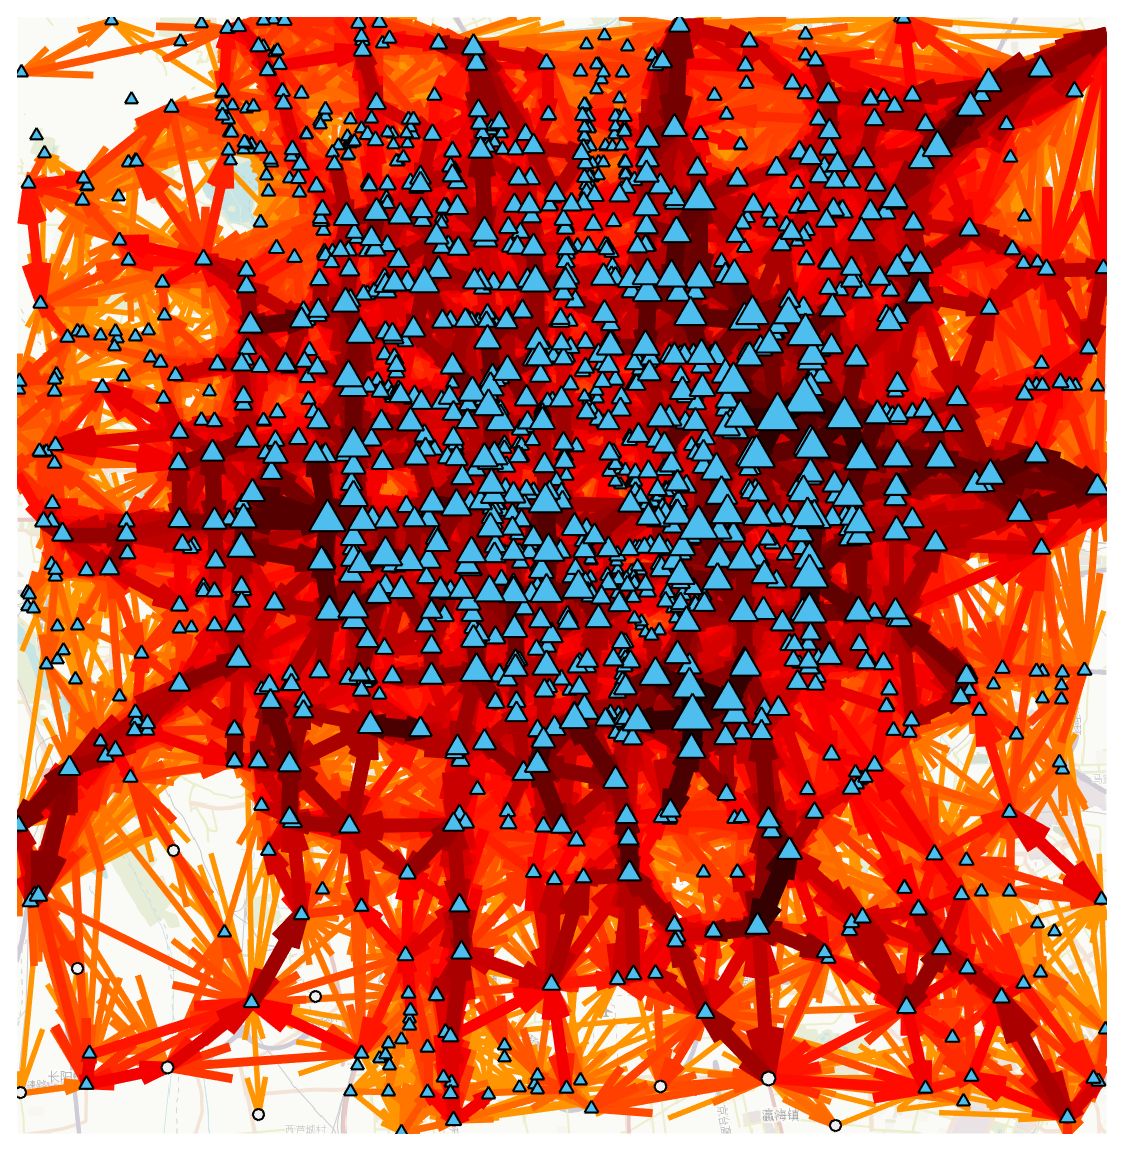
\includegraphics[width=35mm]{pics/tdrive1000with2.eps}\\
\multicolumn{2}{c}{(c) T-drive: $\epsilon = 200$ (m)} & & \multicolumn{2}{c}{(d) T-drive: $\epsilon = 1000$ (m)}\\
\multicolumn{5}{c}{
\begin{minipage}[b]{138mm}\centering

\begin{minipage}[b]{35mm}\centering
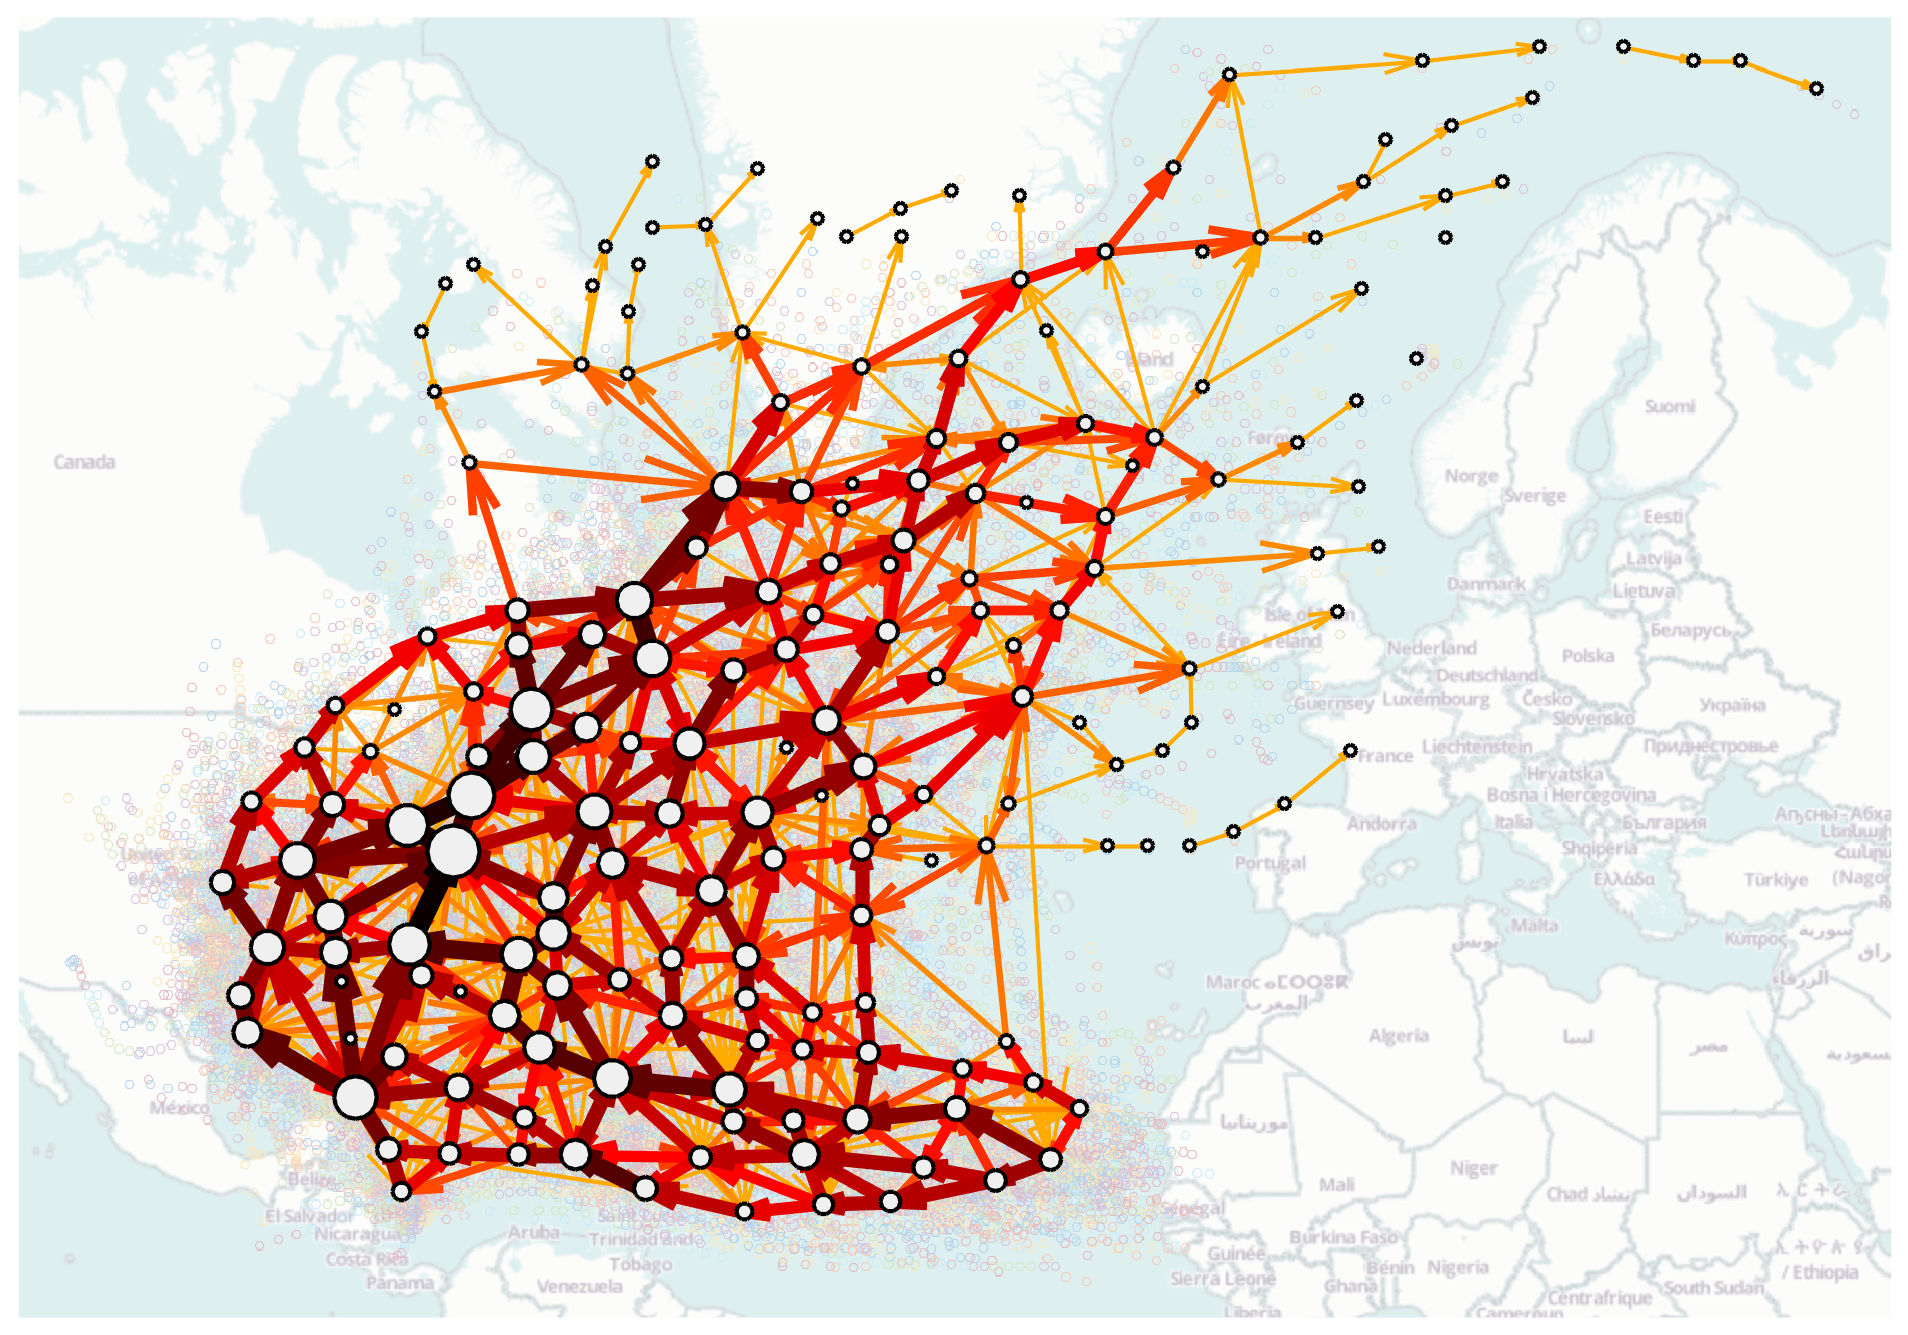
\includegraphics[width=34mm]{pics/Hurricane_2.eps}\\
(e)  $\epsilon = 180$ (km) \\
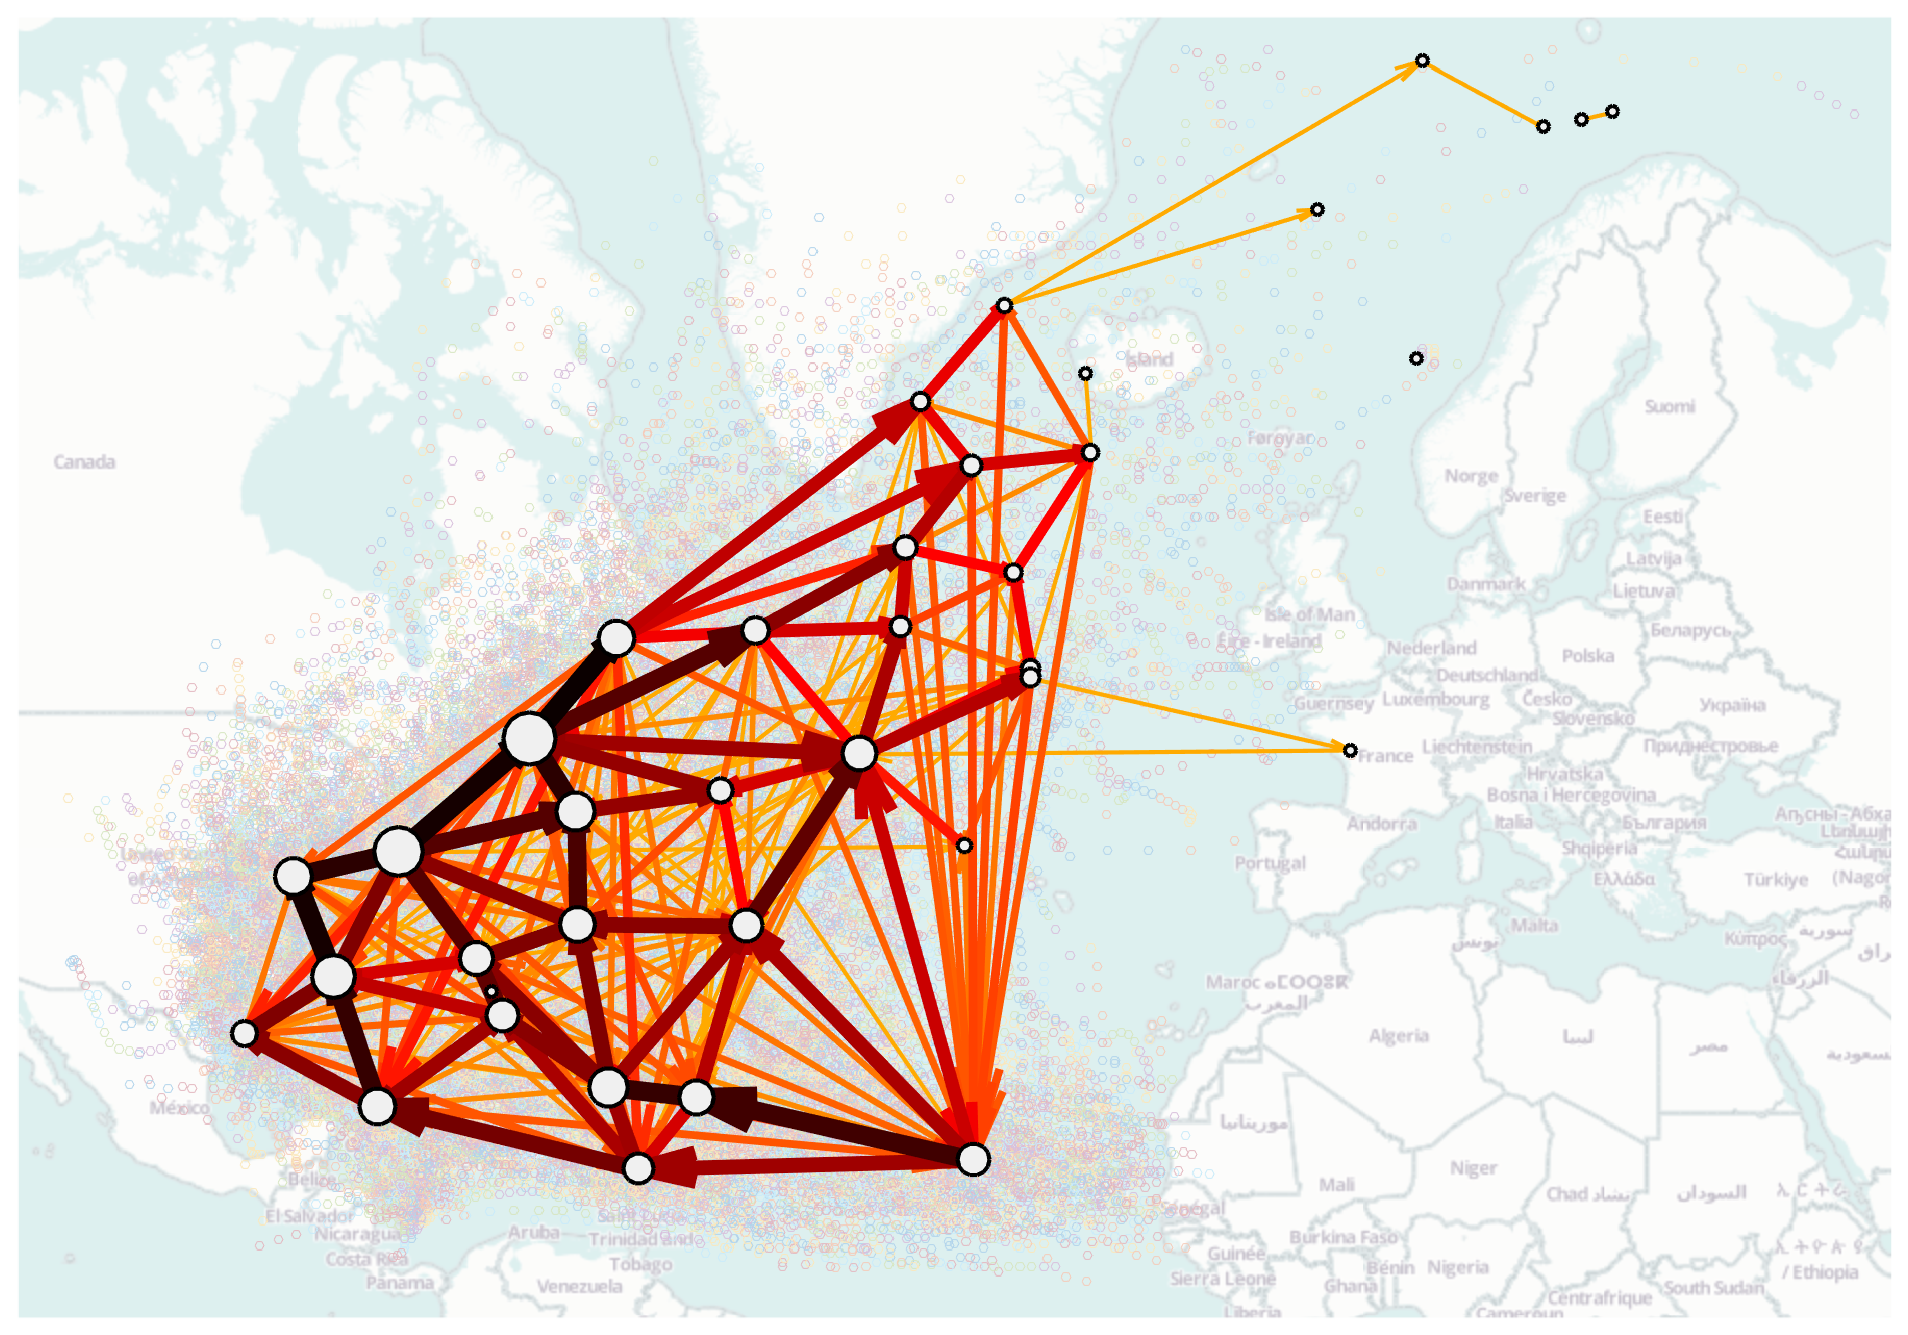
\includegraphics[width=34mm]{pics/Hurricane_4.eps}
(f)  $\epsilon = 540$ (km)
\end{minipage}
\begin{minipage}[b]{101mm}\centering
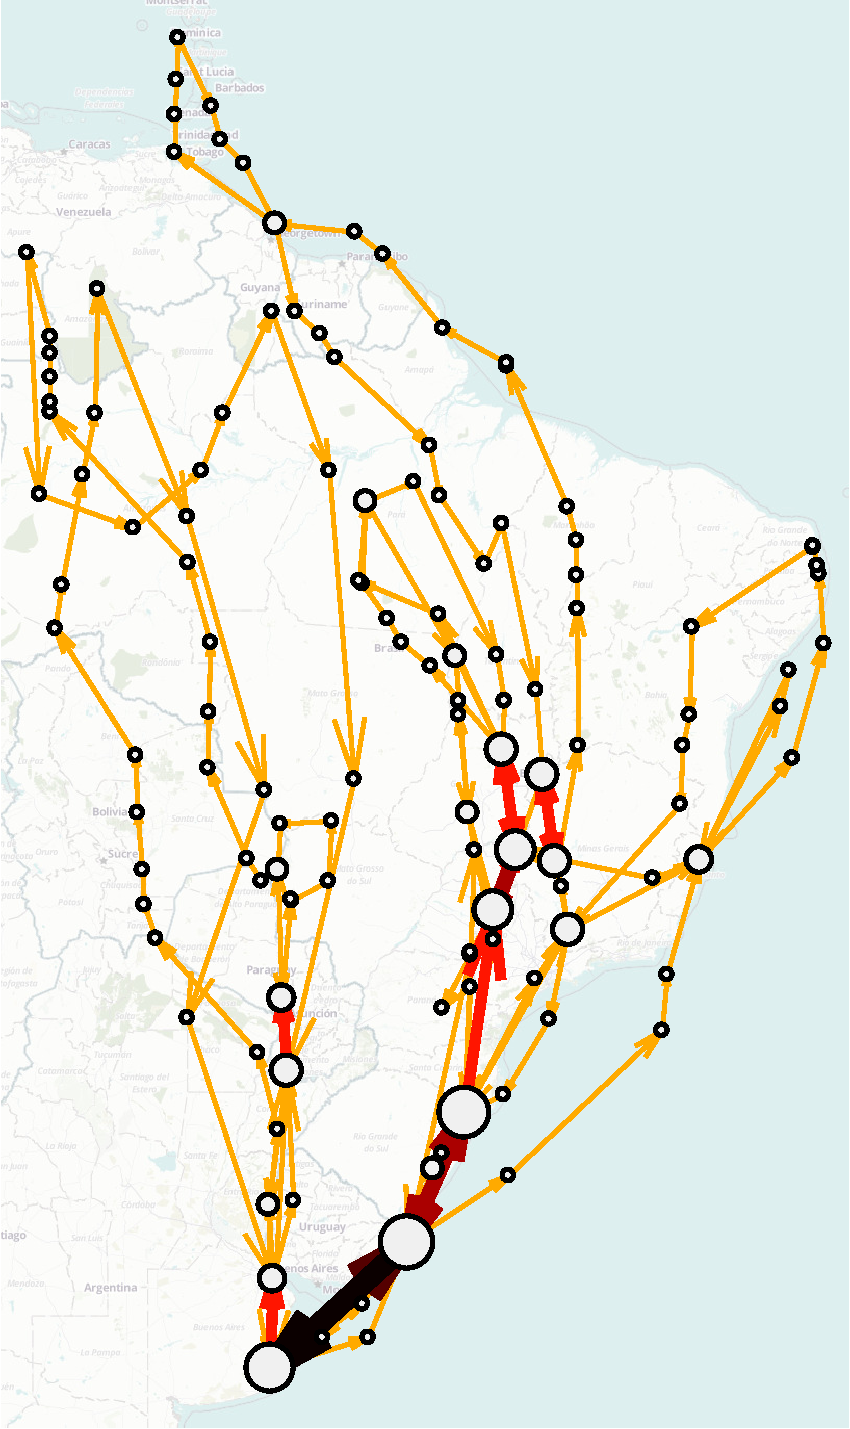
\includegraphics[width=33mm]{pics/Migration_2-eps-converted-to.pdf}
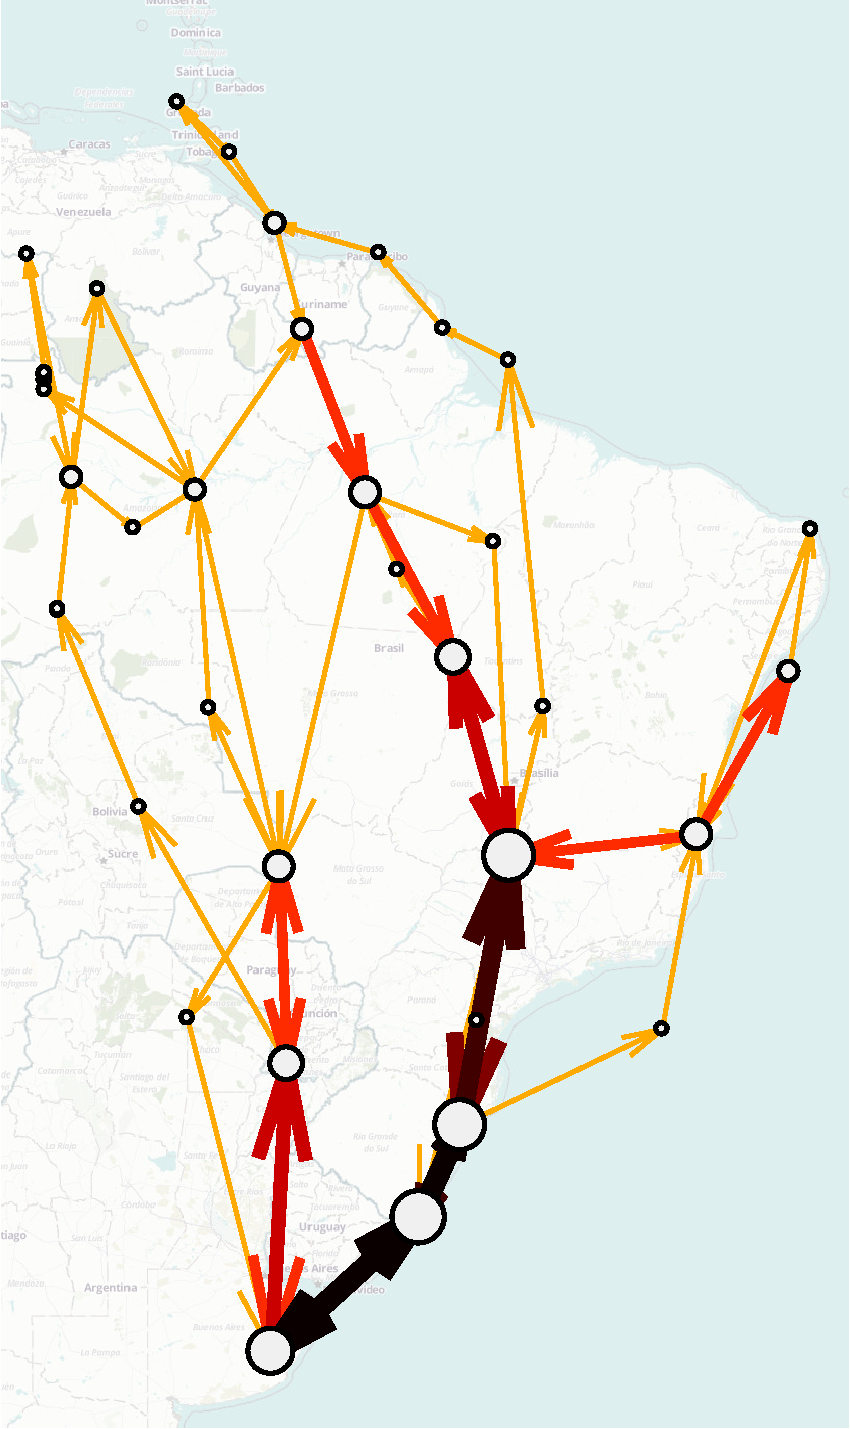
\includegraphics[width=33mm]{pics/Migration_5-eps-converted-to.pdf}
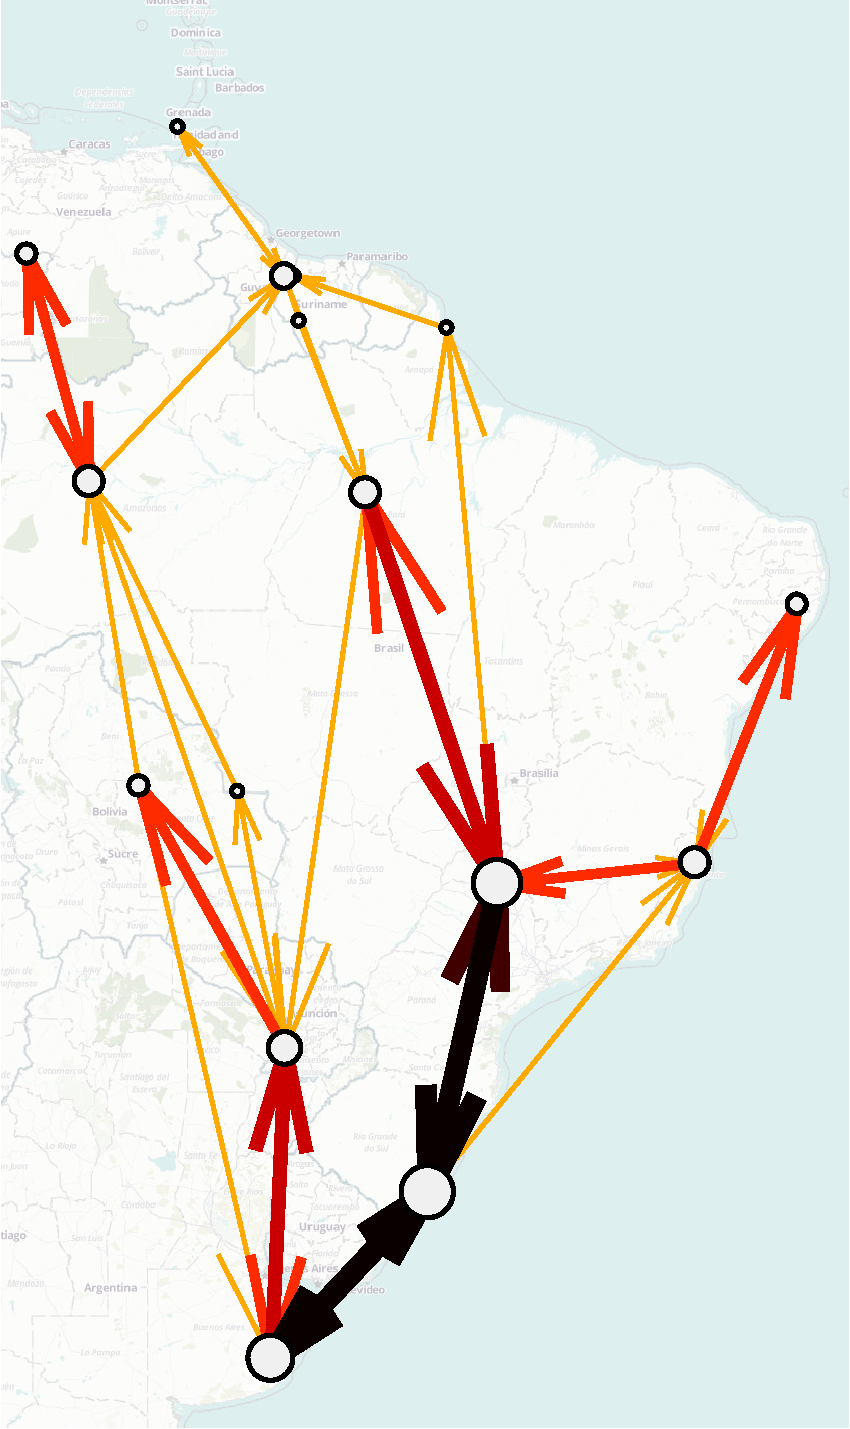
\includegraphics[width=33mm]{pics/Migration_8-eps-converted-to.pdf}\\
(g) $\epsilon = 10$ (km)  ~~~~(h) $\epsilon = 30$ (km) ~~~~ (i) $\epsilon = 50$ (km) \\
\end{minipage}
\end{minipage}
}\\
\end{tabular}
\caption{ROI网络在在不同的数据集上不同误差界的结果。在每一个子图中,左手边的ROI网络是没有固定语义ROI的约束的结果,右边的结果加入了1000个随机选择的十字路口。}
\label{fig:illustration}
\end{figure*}

\smallsection{压缩率分析}
在本节中,我们进行压缩率的比较,以显示\CascadeSync的出色表征能力。注意不同的算法应该使用相同的误差界$\zeta $,以便我们可以直接比较性能。我们在\CascadeSync中设置$\zeta = \epsilon $,这是依据了上面结果中结果将会以以高概率(大于$97\%$)满足这个条件。

\CascadeSync将在Geolife和T-Drive数据上使用两次,其中不同之处在于是否使用了预定义的交叉点(即语义信息)。通过在合理范围内改变误差约束$ \zeta $的值,我们将四个数据集的压缩比呈现在结果\ref{fig:ratio}中。而一些结果ROI网络将在\ref{fig:illustration}中被可视化。

结果中,四个数据集上压缩比的比例是不同的。例如,Geolife和T-drive都是北京的轨迹。然而,Geolife的采样率是T-drive的数百倍。因此,Geolife中包含更多冗余,从而产生非常高的压缩比。图\ref{fig:illustration}(a)-(d)中的ROI网络也显示着这一差异。T-drive的ROI网络比Geolife更复杂,这表明轨道上存在许多空缺区域。

尽管如此,四个模型的压缩比在每个数据集中是可以横向比较的。Douglas-Peucker优于其他模型,我们的\CascadeSync在没有语义ROI中随着误差界的增加而倾向于超越其他模型。重要的是要注意Traclu-MDL呈现扁平的结果,这是因为模型不将误差界作为参数,因此无法控制压缩比。同时,\CascadeSync在具有语义信息下并不擅长控制压缩率,这种现象也可以通过图\ref{fig:illustration}ROI网络揭示出来。通过增加误差界限$\zeta$,正常ROI开始减少,道路交叉点逐渐成为地图上起主导地位的ROI。

实验表明,\CascadeSync具有出色的压缩比和表征能力。现在我们通过比较运行时与其他算法来展示\CascadeSync最显着的特性。我们报告了六种算法对四种真实数据的运行时间。每个算法在每个数据集上运行十次,平均运行时间统计结果如表\ref{tab:times}中所列。请注意,表\ref{tab:times}和图\ref{fig:ratio}中的压缩比是在统一的实验中同时测量的。\CascadeSync比其他五种方法快数千倍。这是因为传统模型逐个压缩轨迹,因此运行时间与数据集中的点成比例。我们的模型在全局范围内进行,因此点数将呈指数级减少,这大大加速压缩过程。




\tabcolsep=0pt
\begin{figure}[!htb]
\centering
% \footnotesize
\begin{tabular}{cc}
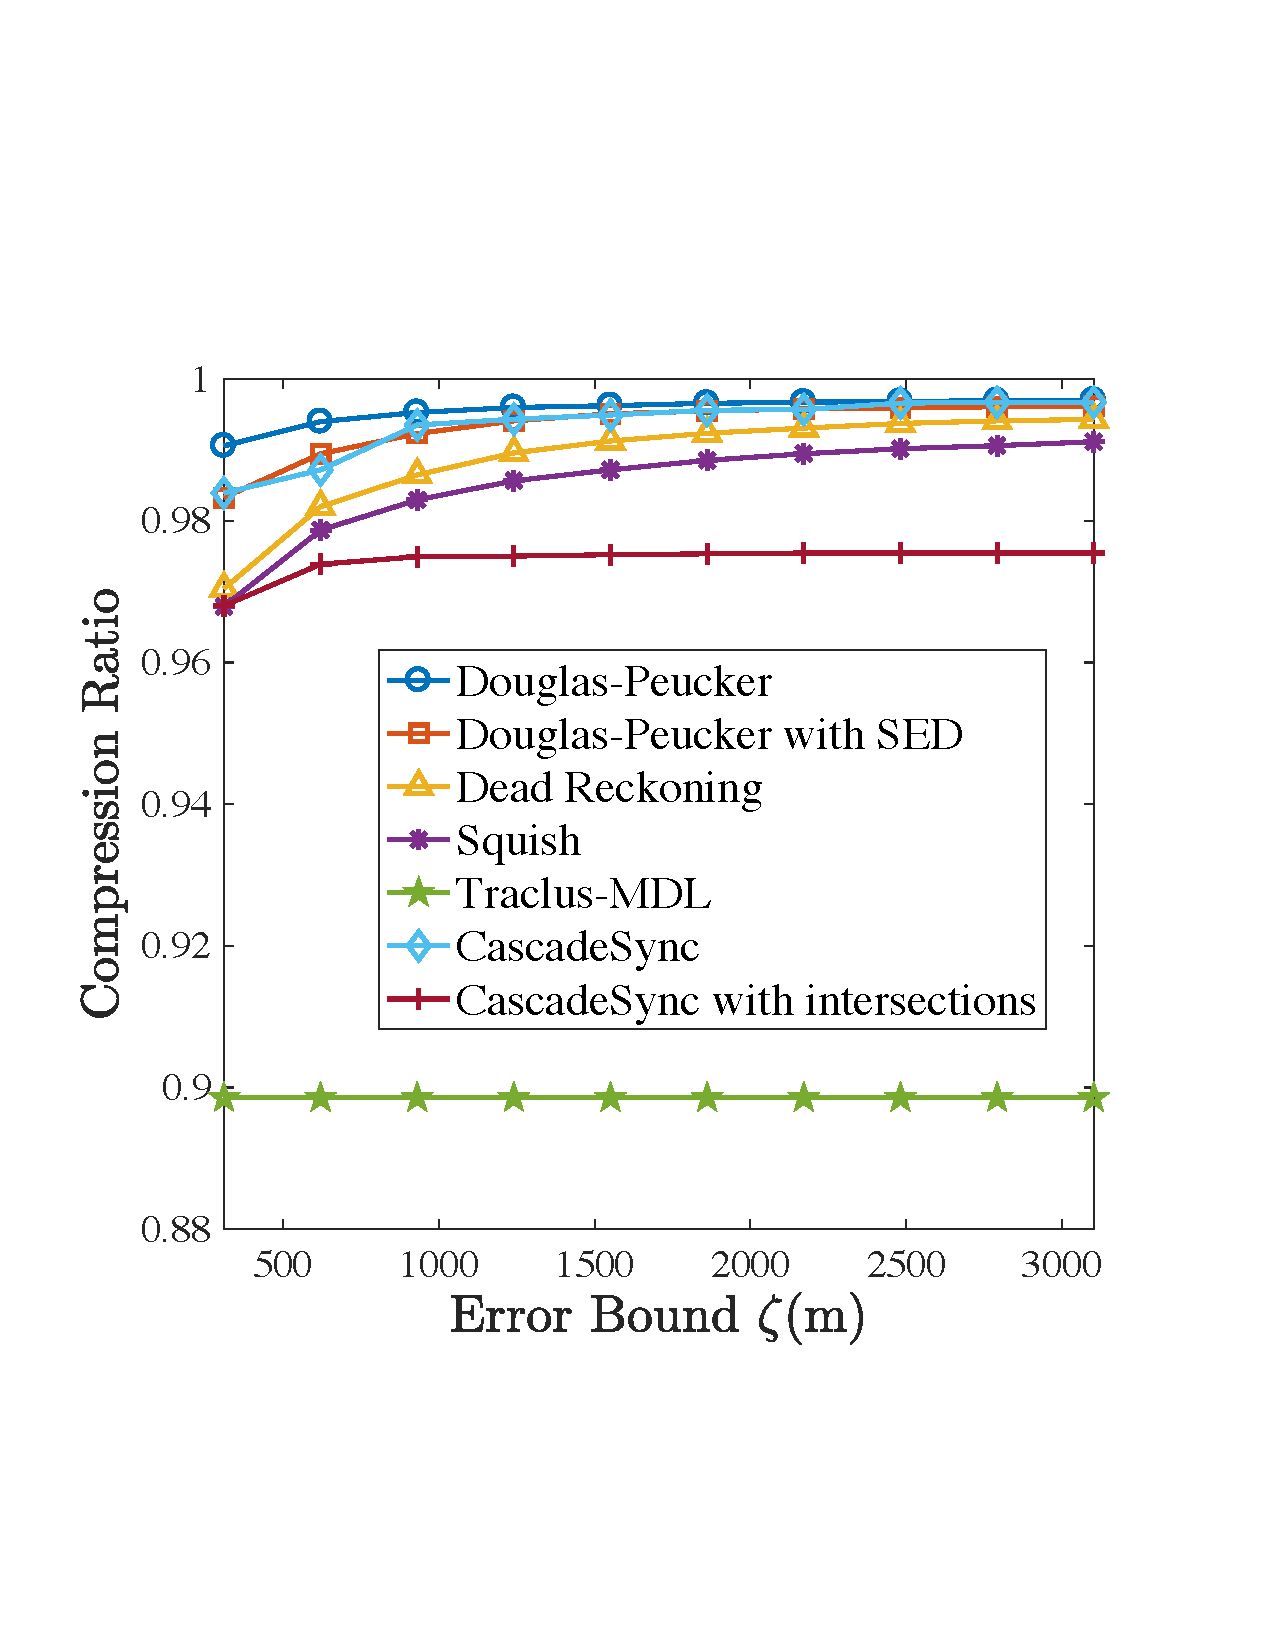
\includegraphics[width=60mm]{pics/geolife.pdf}&
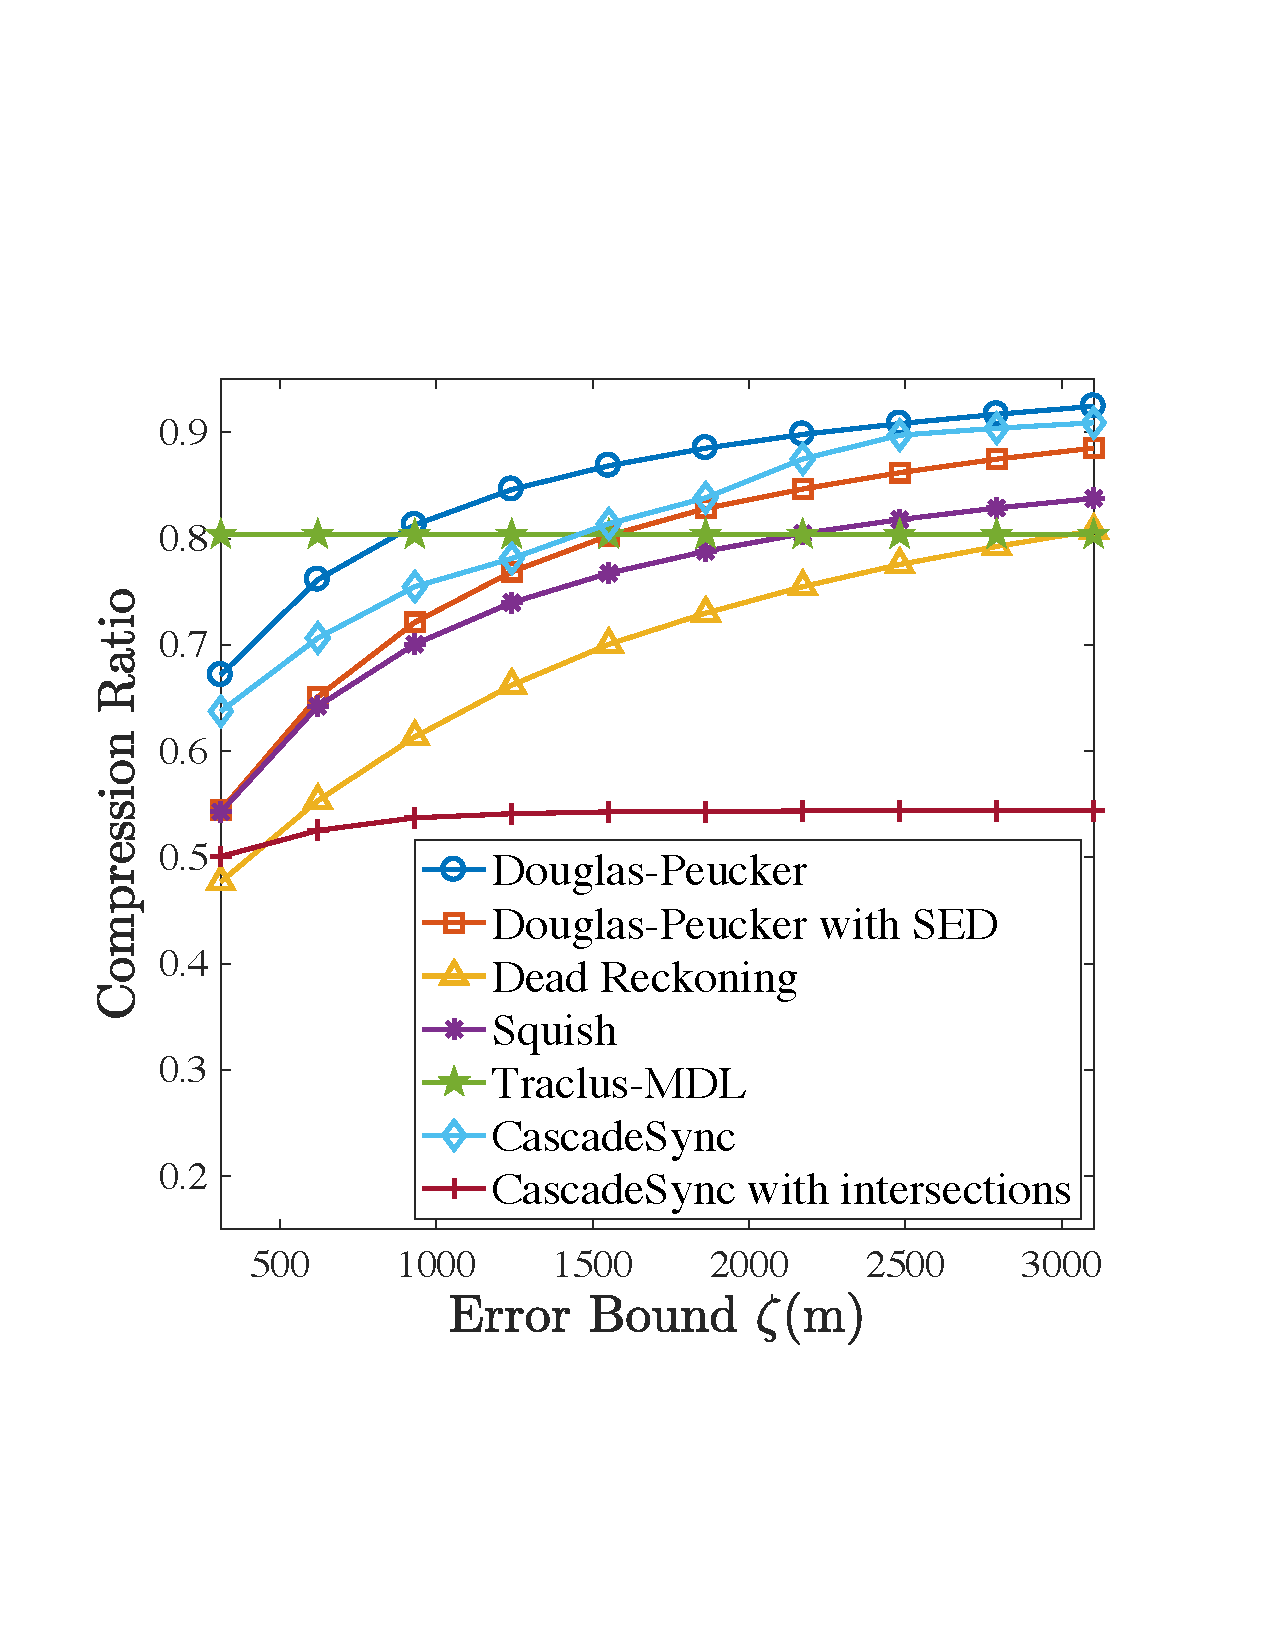
\includegraphics[width=60mm]{pics/tdrive.pdf}\\
(a) Geolife & (b) T-drive \\
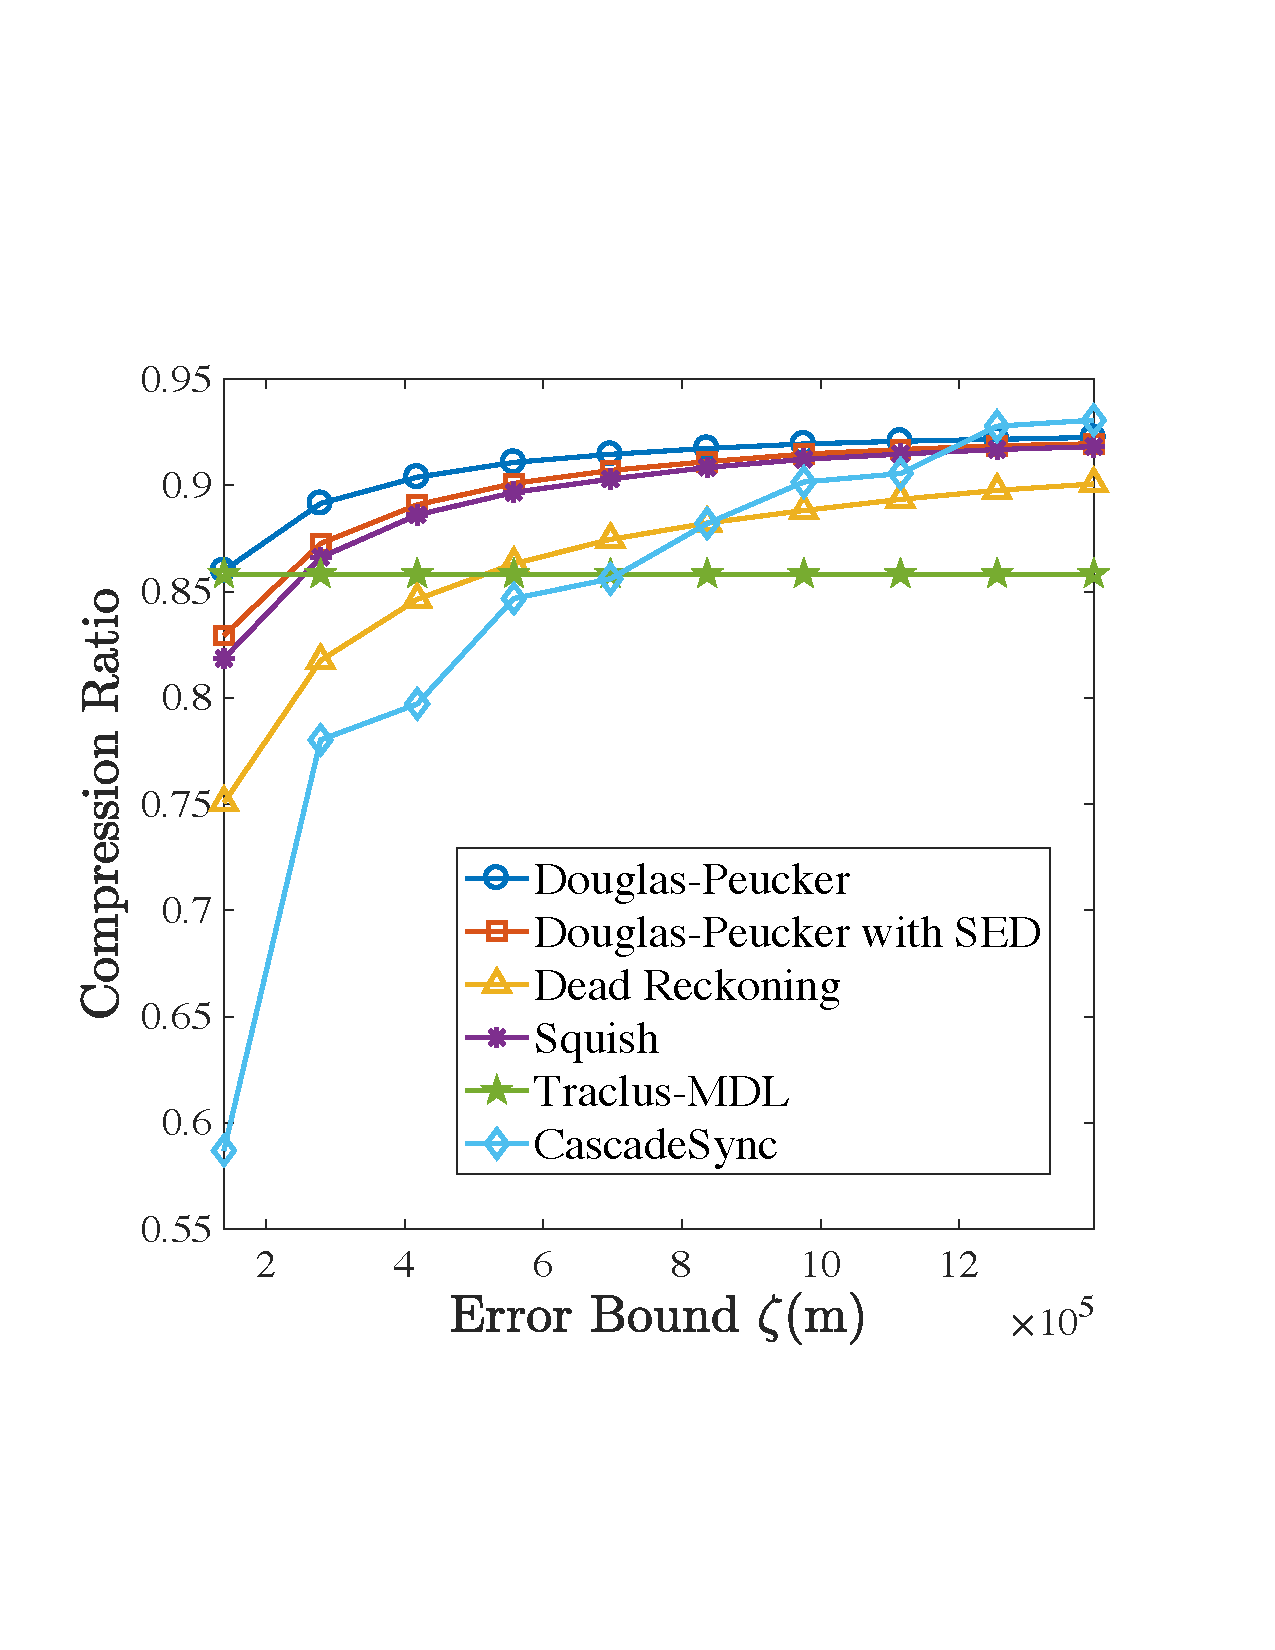
\includegraphics[width=60mm]{pics/hurricane.pdf}&
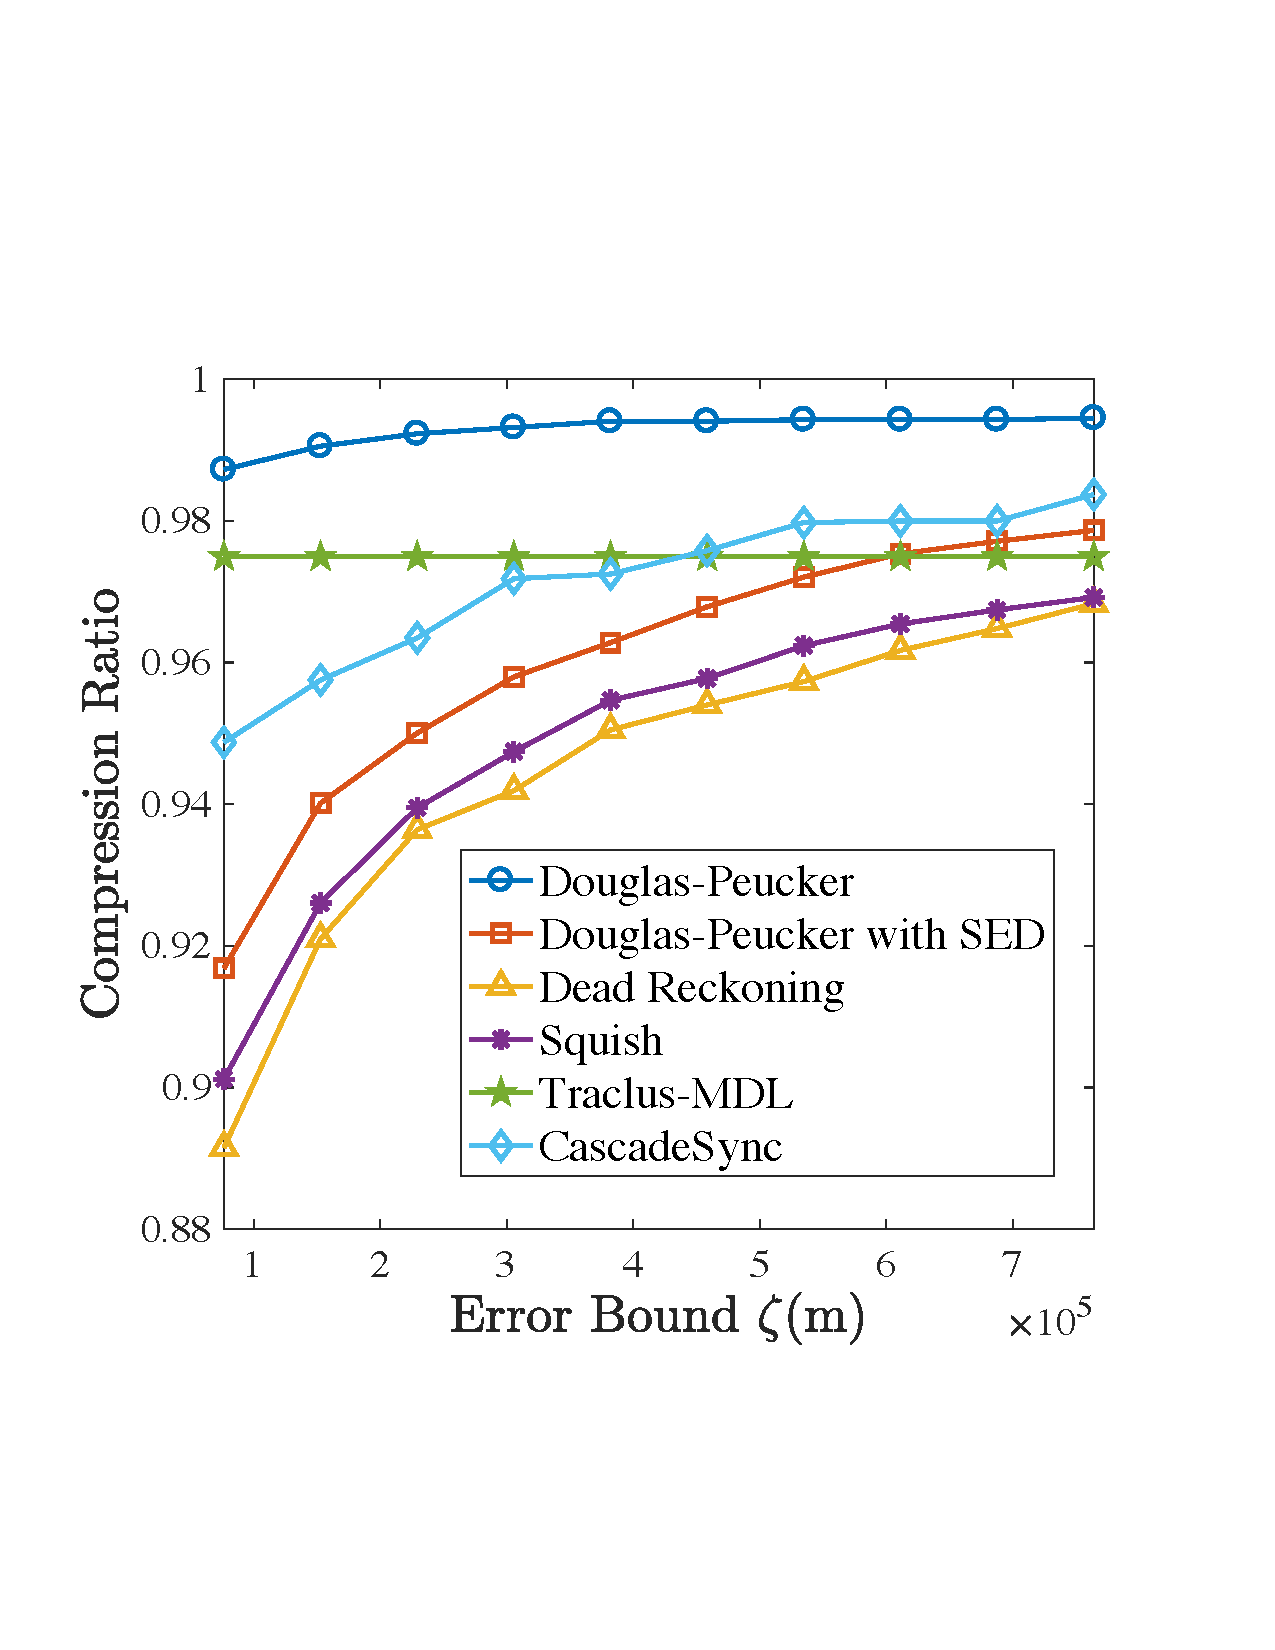
\includegraphics[width=60mm]{pics/Migration.pdf}\\
(c) Hurricane & (d) Migration\\
\end{tabular}
\caption{在四个数据集上压缩率—误差界变化曲线图。}
\label{fig:ratio}
\end{figure}


\tabcolsep=2pt
\begin{table}[!htb]\renewcommand{\arraystretch}{1.3}
\vspace{1mm}
\caption{在四个数据集上的速率对比结果。单位:秒。}
\center
\small
\begin{tabular}{lcccccc}
\hlinew{1pt} \textbf{}& \textbf{~~DP~~}& \textbf{~~DP-SED~~} & \textbf{~~DR~~} & \textbf{Squish} & \textbf{Traclus-MDL} & \textbf{CascadeSync}\\ 
\hlinew{1pt}
\textbf{Geolife}  & 6100.42 & 36621.08 & 14525.53 & 14712.10 & 6357.91 & \textbf{15.38}\\
\textbf{Tdrive}   & 2288.57 & 35422.91 & 5101.41 & 5289.05 & 2344.51 & \textbf{7.51}\\
\textbf{Hurricane}& 16.46 & 49.80 & 30.98 & 33.54 & 13.78 & \textbf{0.42}\\
\textbf{Migration}& 1.79 & 12.09 & 4.40 & 4.44 & 2.28 & \textbf{0.10} \\
\hlinew{1pt}
\end{tabular}
\label{tab:times}
\end{table}


\tabcolsep=5pt
\begin{table*}[!htb]\renewcommand{\arraystretch}{1.3}
\caption{Geolife数据集上的时空查询结果。}
% \vspace{1mm}
\center
\small
\begin{tabular}{c|c|c|c|c|c}
\hlinew{1pt}
\multicolumn{3}{c|}{\textbf{轨迹时空查询}} & \multicolumn{3}{c}{\textbf{轨迹条数}} \\
\hlinew{1pt}
编号 & 地点 & 时间范围 & $\epsilon = 500m$ & $\epsilon = 1000m$ & $\epsilon = 3000m$\\
\hlinew{.85pt}
\multirow{2}{*}{1}& 北京大学 & \multirow{2}{*}{2008-11-28,2009-01-07} &\multirow{2}{*}{3} & \multirow{2}{*}{8} & \multirow{2}{*}{51}\\
& 金融街 & & & & \\
\hline
\multirow{2}{*}{2}& 王府井 & \multirow{2}{*}{2009-02-14,2009-03-20} &\multirow{2}{*}{4} & \multirow{2}{*}{18} & \multirow{2}{*}{44}\\
& 北京西站 & & & & \\
\hline
\multirow{3}{*}{3}& 天安门广场 & \multirow{3}{*}{2009-01-27,2009-02-25} &\multirow{3}{*}{0} & \multirow{3}{*}{2} & \multirow{3}{*}{9}\\
& 北京站, & & & & \\
& 国家体育馆 & & & & \\
\hline
\multirow{3}{*}{4}& 中关村 & \multirow{3}{*}{2008-06-18,2008-06-22} &\multirow{3}{*}{1} & \multirow{3}{*}{2} & \multirow{3}{*}{12}\\
& 光熙门, & & & & \\
& 建国门 & & & & \\
\hline
\multirow{3}{*}{5}& 天坛公园 & \multirow{3}{*}{2008-04-02,2009-11-23} &\multirow{3}{*}{15} & \multirow{3}{*}{139} & \multirow{3}{*}{578}\\
& 故宫, & & & & \\
& 北海公园 & & & & \\
\hlinew{1pt}
\end{tabular}
\label{tab:retrieval}
\end{table*}

\tabcolsep=1pt
\begin{figure*}[!t]
\centering
% \footnotesize
\begin{tabular}{ccc}
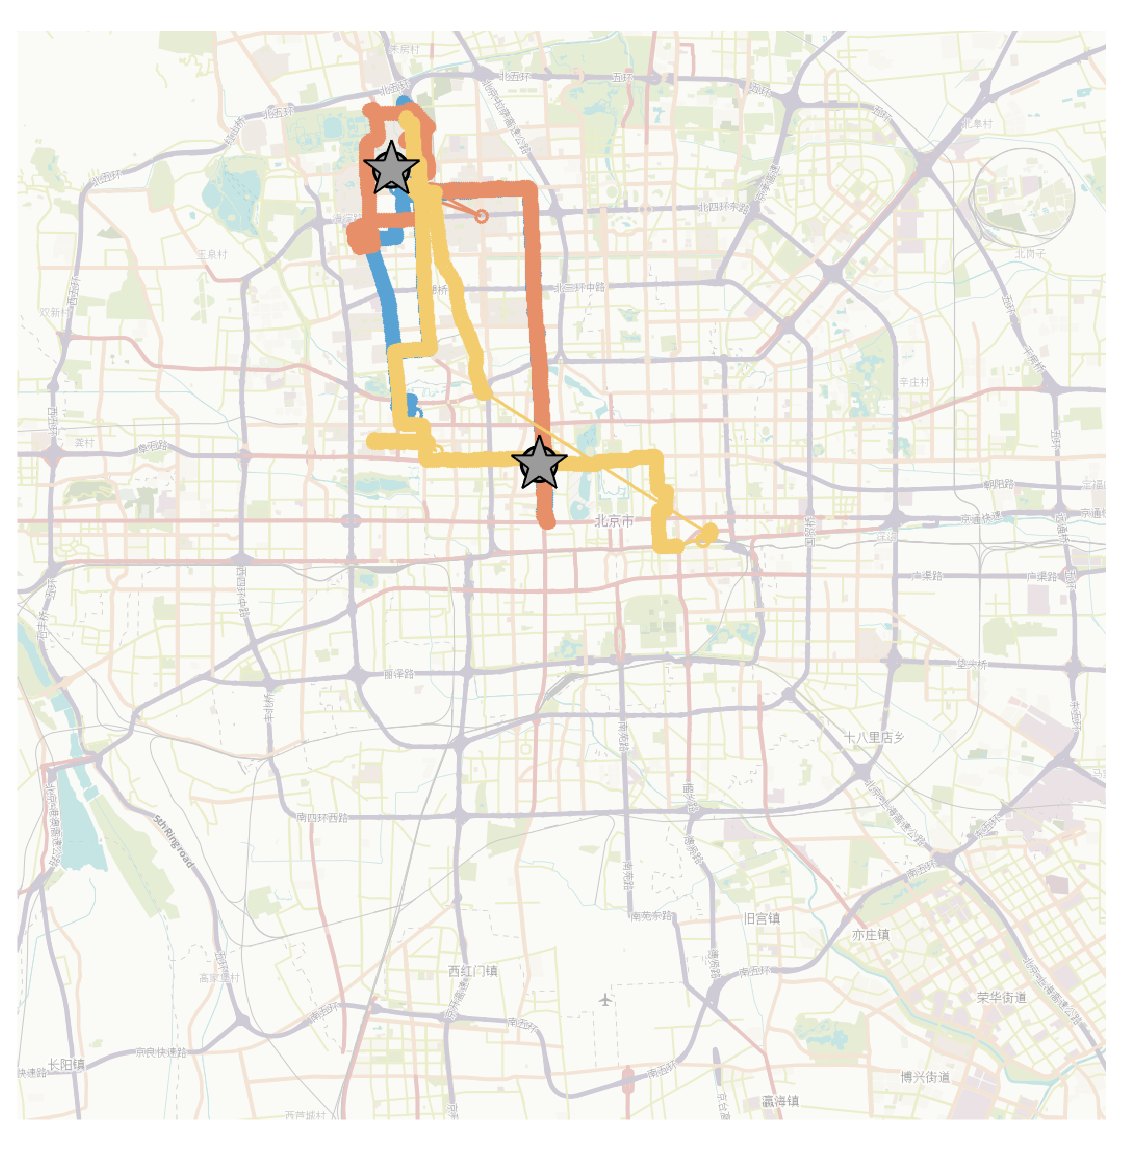
\includegraphics[width=48mm]{pics/q500.eps}&
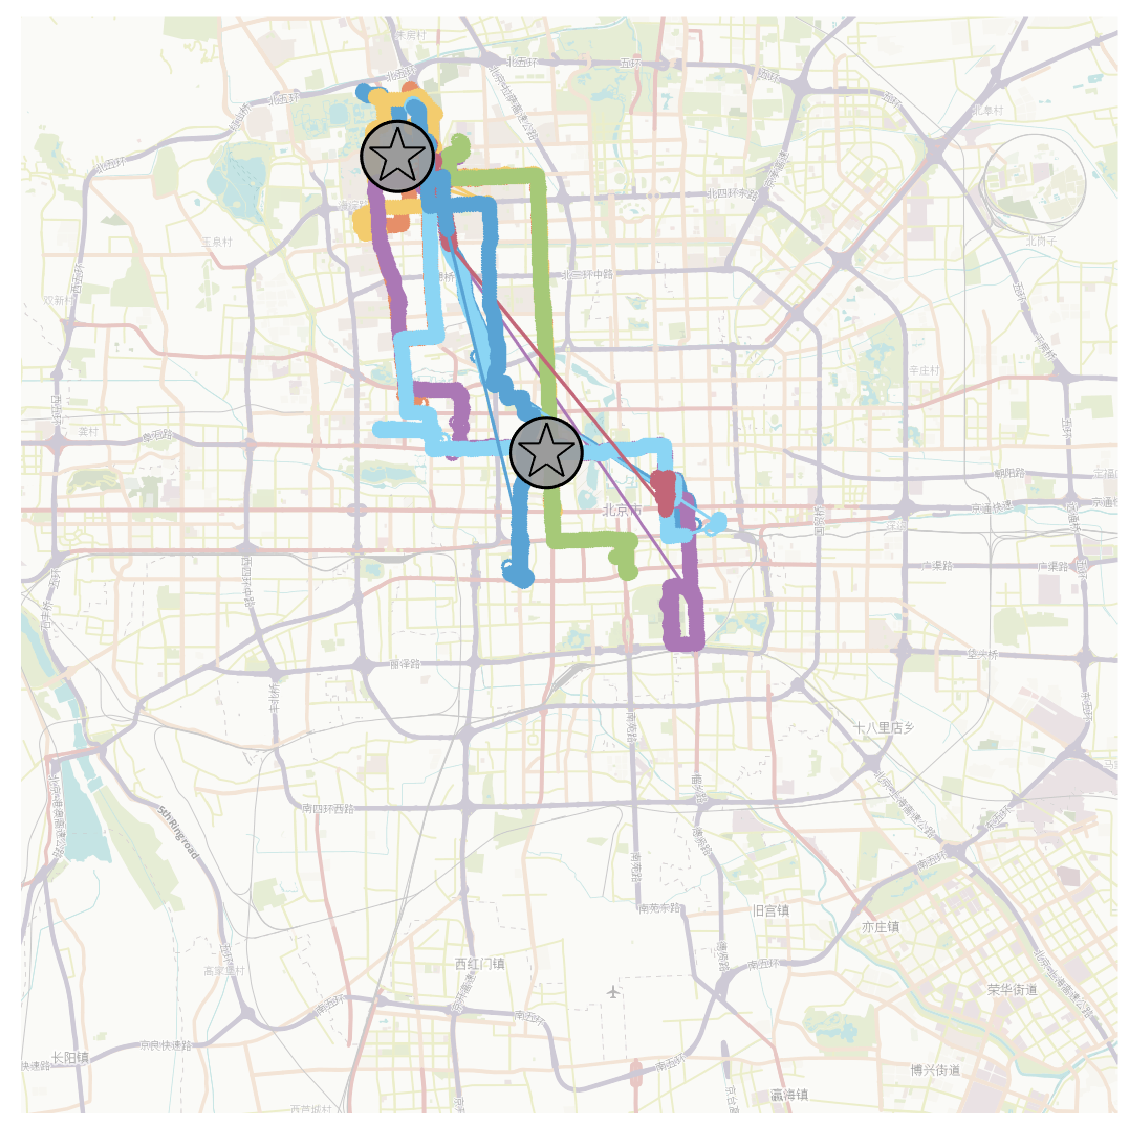
\includegraphics[width=48mm]{pics/q1000.eps}&
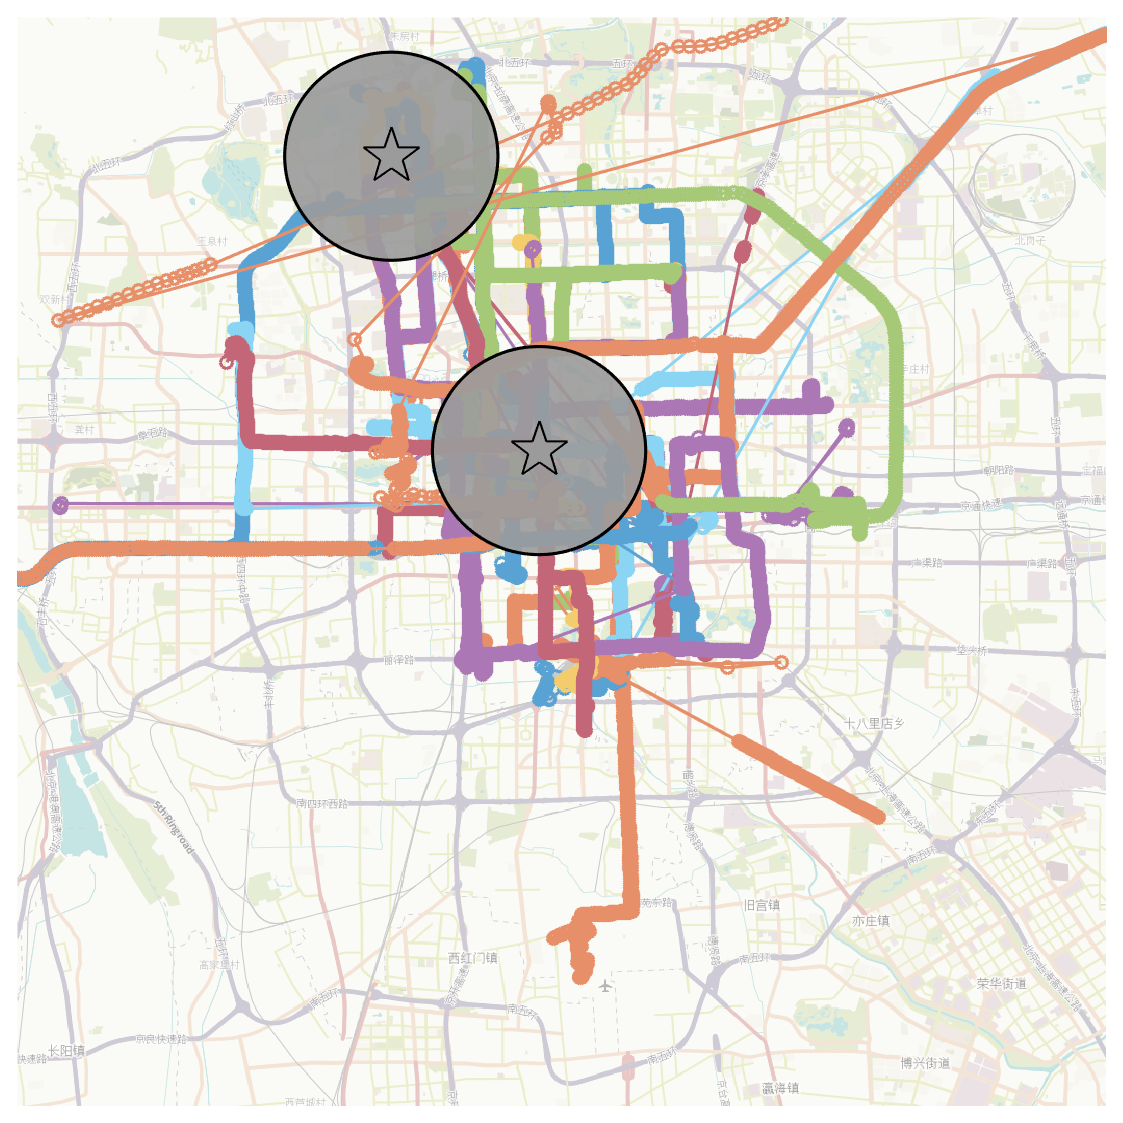
\includegraphics[width=48mm]{pics/q3000.eps}\\
(a) $\epsilon = 500m$, \#Traj.=3 & (b) $\epsilon = 1000m$, \#Traj.=8 & (c) $\epsilon = 3000m$, \#Traj.=51  \\
\end{tabular}
\caption{不同搜索范围的轨迹时空轨迹检索结果。这里检索了两个地点北京大学和金融街。 时间范围从2008-11-28到2009-01-07。 圆的半径表示交互范围范围$\epsilon$。}
\label{fig:queryResult}
\vspace{2mm}
\end{figure*}

\smallsection{轨迹的时空查询}
ROI网络是轨迹数据的一种紧凑表示,在ROI网络上可以总结全局信息和特殊语义信息,这可以促进后续应用。在本节中,我们以时空检索任务为例。给定城市中的一组地标或区域以及时段,我们检索在相应时段内通过所有这些地段或者区域的轨迹。由于我们的多层次ROI网络记录了通过轨迹的访问时间,因此可以通过在已有ROI网络上应用算法\ref{alg:query}来轻松检索轨迹。

为简单起见,我们只说明Geolife上的查询结果,并执行五个查询。由于在 Geolife数据上,大多数轨迹都位于微软亚洲研究院(MSRA)和一些大学的校园附近,因此覆盖整个北京城市的轨迹很少。这里我们只考虑三个范围(500米,1000米和3000米)。如在图\ref{fig:queryResult}中给出2008-11-28至2009-01-07的第一个检索结果。当$\epsilon$设置为500米时,穿过北京大学和金融街的共同轨迹只有3条,而随着交互范围$ \epsilon $的增加,结果数量自然会上升。

实验表明,在给定的特定点和相应的时间范围内,查询结果可以以不同的分辨率可视化,这可以对后续应用的开展帮助很大。


\section{本章小结}
% \vspace{-2mm}
本章中我们为了将给定的轨迹数据集表示为多层次ROI网络,提出了基于同步的语义轨迹压缩算法\CascadeSync。在同步聚类的概念下,\CascadeSync
算法允许在可用语义信息存在与缺失的情况下都能产生多分辨率轨迹抽象表征结果(分层ROI网络)。 更重要的是,抽象的轨迹表示很好地保留了全局轨迹信息,并且很方便各种语义信息的集成。而对于轨迹流,我们开发了一种简单的基于窗口合并以及分离的方法来进行在线处理。我们在人工数据和四个真实数据集上进行多项实验,证明了提出方法相比起国际主流方法的有效性和高效性。
\newpage\mbox{}\thispagestyle{empty}\newpage

% % !Mode:: "TeX:UTF-8"

\chapter{分布式轨迹语义表征}
\label{chapter:main2}

要在轨迹上进行信息挖掘,首先需要在轨迹上定义一个空间,使得轨迹中蕴含的语义可以得到表示,同时使不同轨迹之间感兴趣的相似度能够得到衡量。在不同的场景下,研究者们纷纷提出利于自己算法运行的轨迹表征方法,然而根据应用定下的表征通常没有普适性。为此,本文提出了一种鲁班的轨迹表征方法,使得各种感兴趣的语义都能根据需求融入此表征方法中,进而为后续轨迹挖掘任务打下基础。


\section{问题描述}
如上文所述,传统的轨迹挖掘算法汇总,轨迹通常有三种表征方式:基于采样点的表征、基于线段的表征以及基于特征的表征。然而这三种表征方式在现在的挖掘需求中都有不足:主要关注地理信息,几乎没有考虑具体的语义知识。因此,在表征上建立的索引系统将给后续挖掘任务带来很多限制。

为了衡量语义相似性,应该为轨迹数据创造一种新的表征,并在这种表征上定义新的轨迹相似性度量标准。举一个例子,图\ref{fig:introduction}(a)显示了葡萄牙波尔图的三个出租车轨迹(即$ T_1, T_2$和$T_3 $)。 如果我们只考虑三个轨迹的几何属性,$ T_1 $和$ T_2 $之间的相似性高于$ T_2 $和$ T_3 $之间的相似性。但是,通过考虑城市的交通系统(即结构信息)和区域功能(即领域知识), 由于这两条轨迹都表明了从农村地区到市中心的高速公路运输,而$T_1$意味着从机场到海滨地区的国家公路,则可以得出$ T_2 $更类似于$ T_3 $的结论(图\ref{fig:introduction}(b))。

在本章中,在上一章节\Cascade算法的输出的多层次ROI网络的基础上,我们利用网络的拓普信息、轨迹的时间信息以及其他的领域知识,用一个层次嵌入模型将ROI网络上的节点嵌入到一个隐空间中,使之有定长的表征。这个过程展现在图\ref{fig:introduction}(c)中。在该表征基础上,语义检索任务可以被铸造为通过简单地计算两个向量之间的欧几里德距离来搜索最相似的向量到目标向量的问题。

\tabcolsep=0.5pt
\begin{figure}[!htb]
\centering
\begin{tabular}{cc}
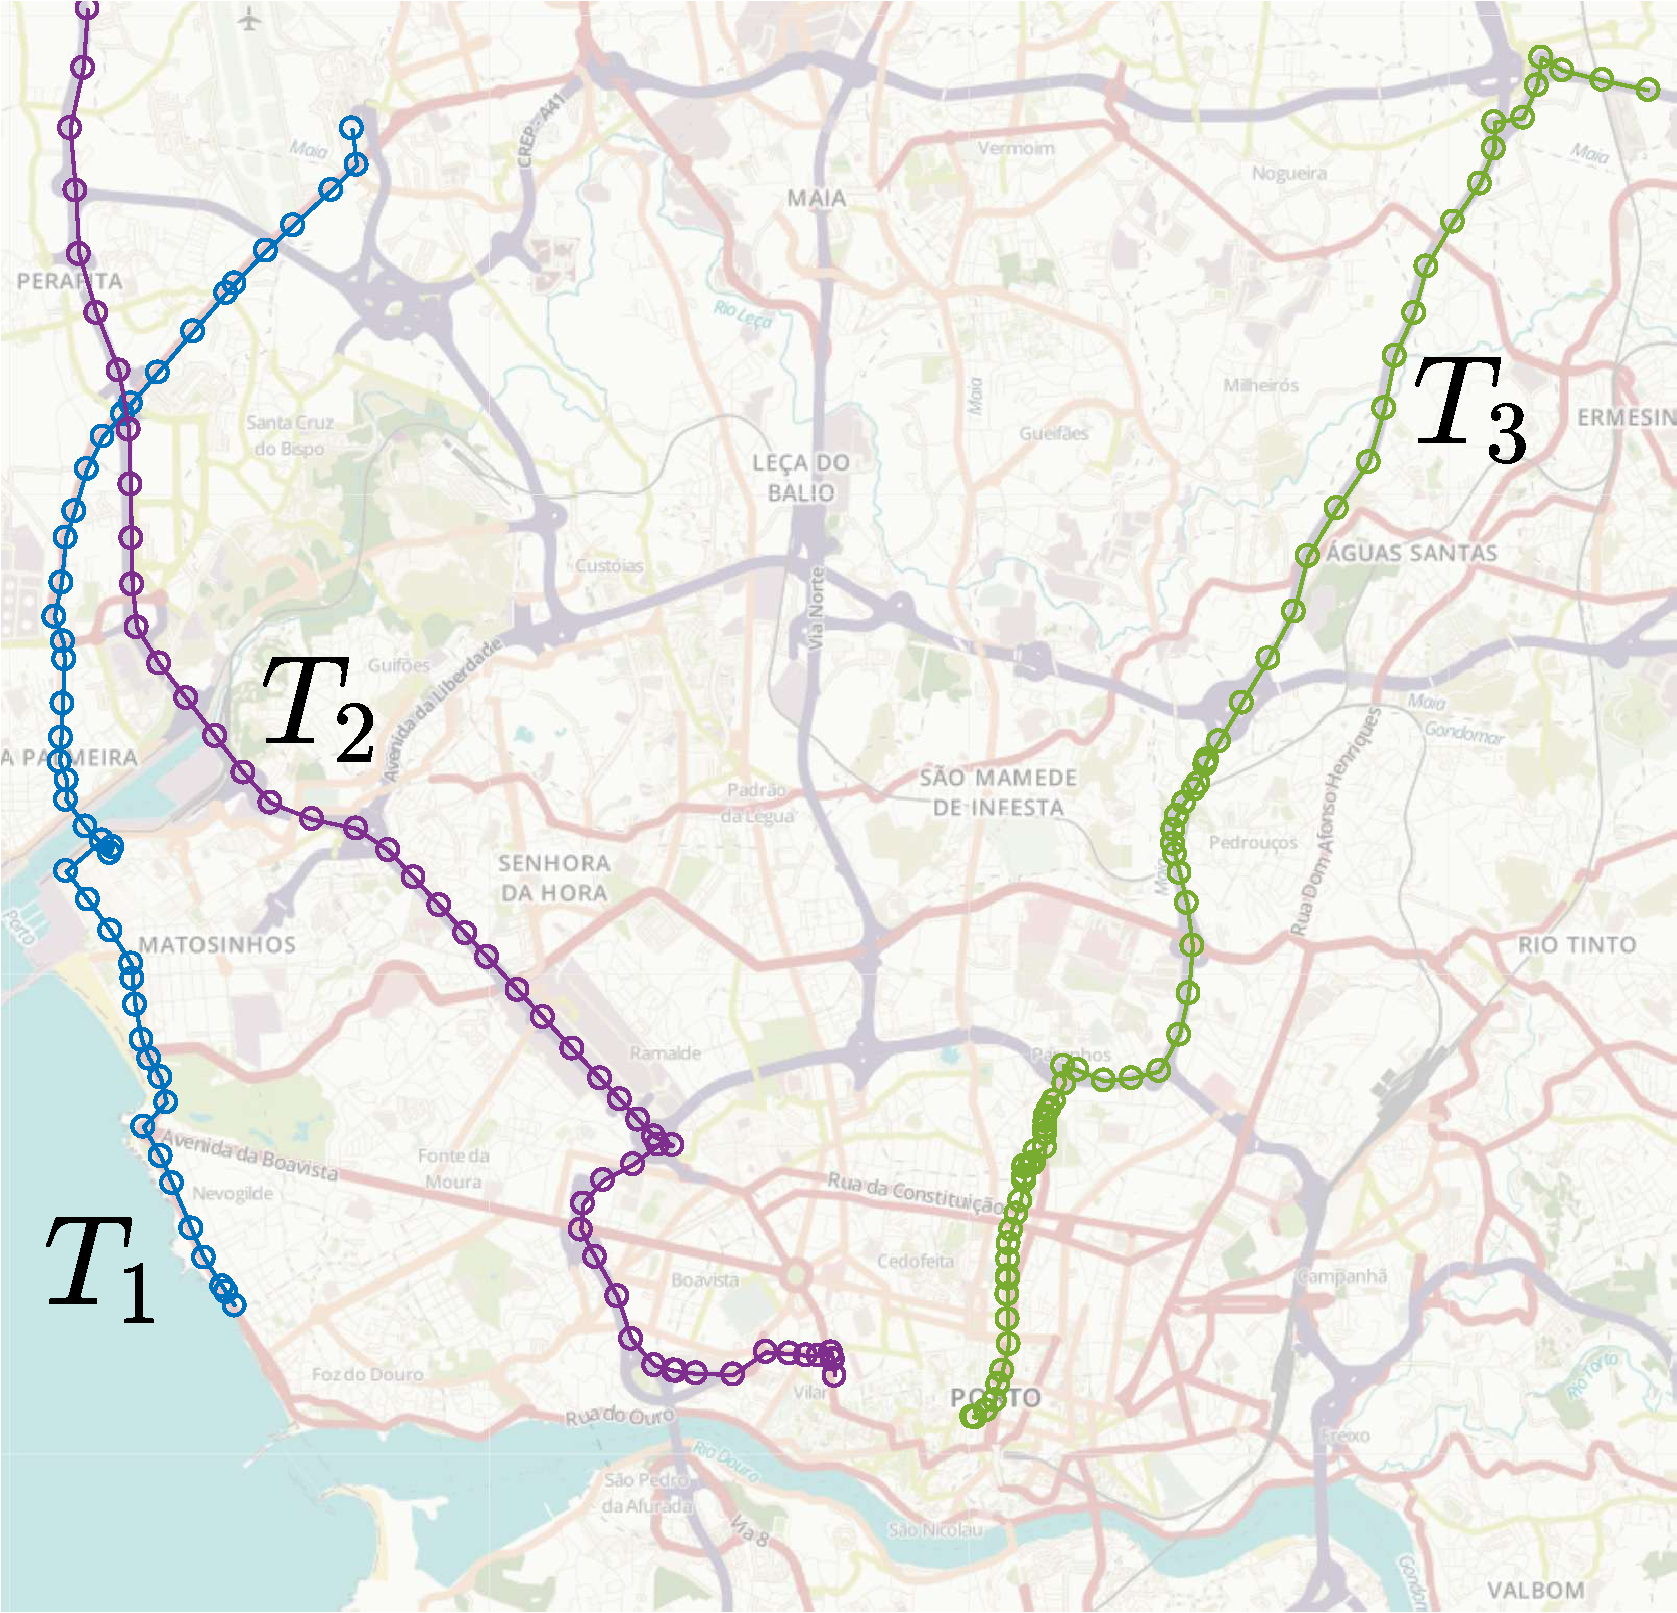
\includegraphics[width=50mm]{pics/introduction1.pdf} & 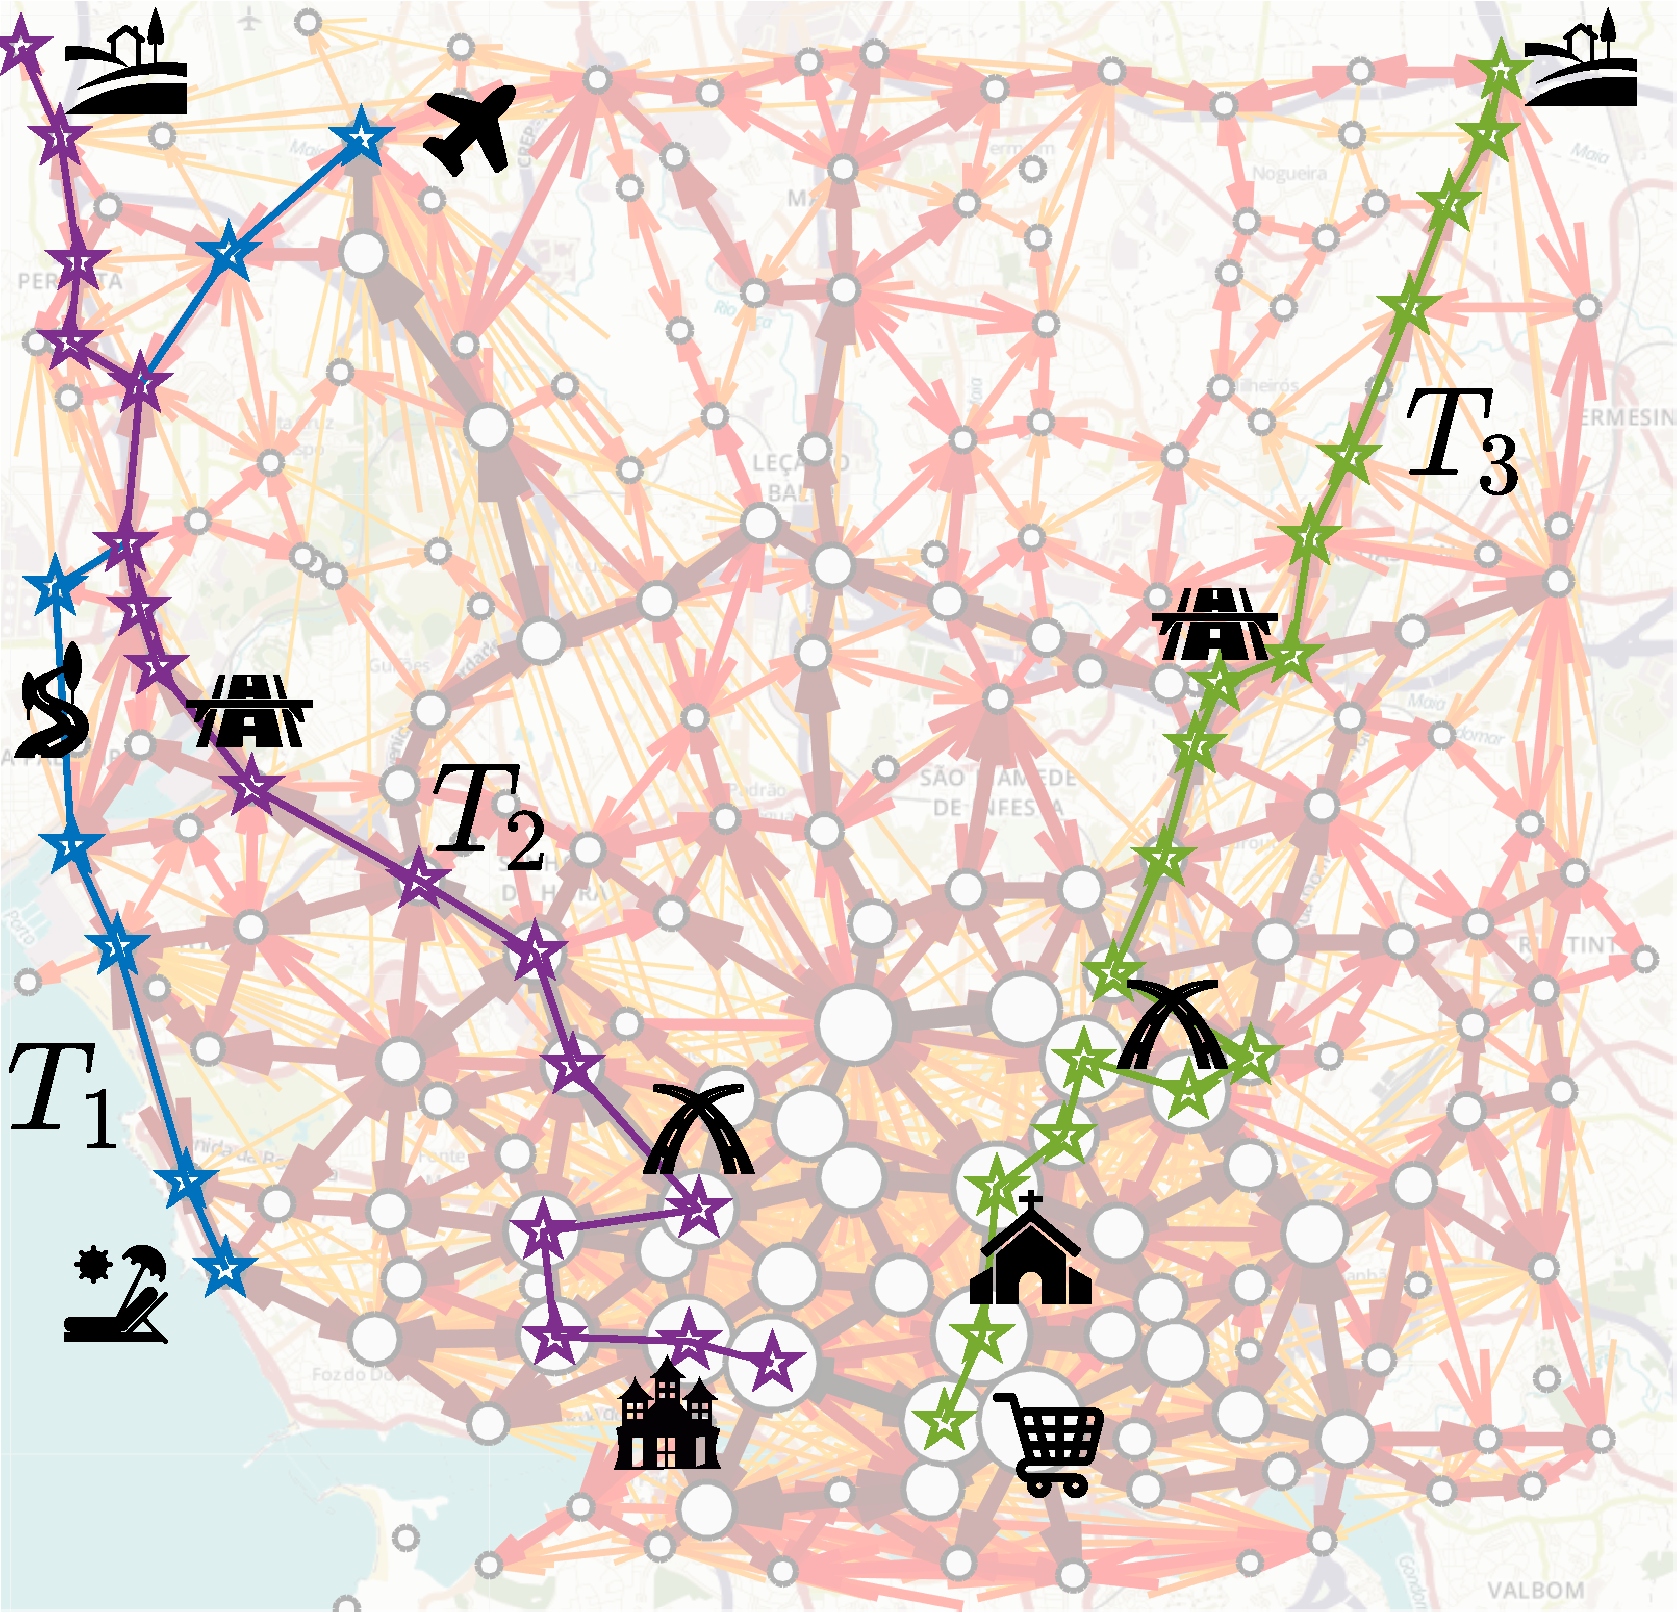
\includegraphics[width=50mm]{pics/introduction2_w.pdf}\\
\multicolumn{2}{c}{\includegraphics[width=100mm]{pics/introduction.pdf}}
\end{tabular}
% \vspace{-2mm}
\caption {轨迹分布式语义表征示意图。(a)葡萄牙波尔图市的三条出租车轨迹;(b) 三条轨迹被\Cascade转换为了ROI序列的表示;(c)将地理序列表示转换为分布式向量表征。}
% \vspace{-3mm}
\label{fig:introduction}
\end{figure}


\section{ROI网络上分布式ROI与轨迹语义嵌入模型}
在上一章的\Cascade算法作用在轨迹数据集上,提取出分层ROI网络之后,每条轨迹将被表征为网络的每个层上的ROI序列。受自然语言处理(NLP)中的词嵌入方案的启发,我们提出了一种嵌入模型,用于进一步将ROI和轨迹转换为语义空间中的连续向量,从而揭示轨迹数据中隐藏的语义信息。

\subsection{单层语义ROI嵌入模型}
嵌入模型的关键是选择给定对象的邻域或上下文,以便可以获得对象之间的关系或者相似度。因此,我们从两个方面考虑ROI的嵌入邻居:几何邻居和语义邻居。

\smallsection{几何邻居}
给定一个ROI,其几何邻居是围绕该ROI的在ROI网络被轨迹以$W$跳能连接起来的其他ROI。 图\ref{fig:context}用$W =2$的几何邻居来作为展示,被绘作绿色和蓝色圆圈。例如,${ROI}_k $是$ {ROI} _i $的几何邻域之一。

\smallsection{语义邻居}
由于ROI不仅仅是网络上的节点,它还代表了一个富含各种语义信息的区域。 为了对丰富的语义进行编码,我们从以下角度定义给定ROI的语义邻域:

\tabcolsep=1pt
\begin{figure*}[!t]
\centering
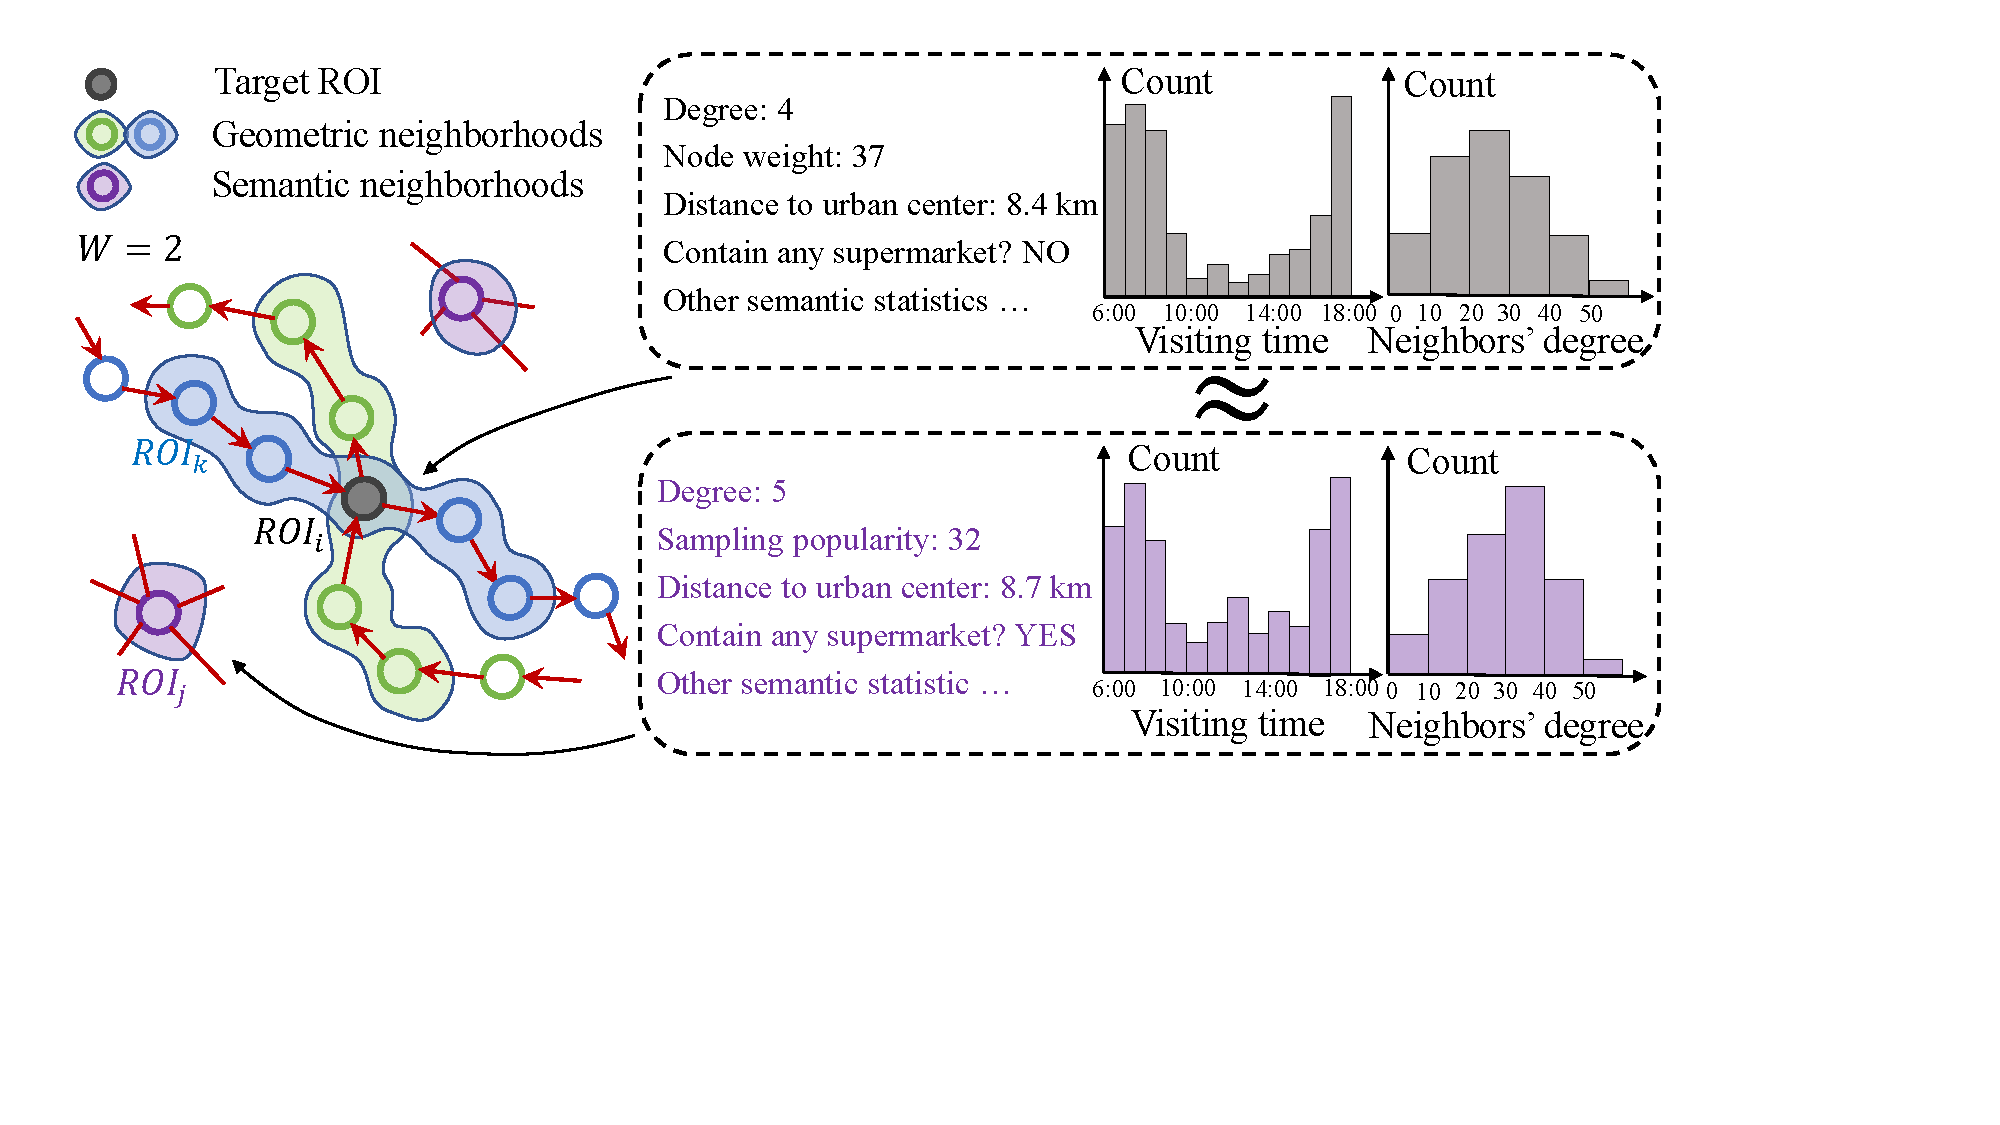
\includegraphics[width=130mm]{pics/embedding.pdf}
\caption {ROI两种邻居示意图。}
% \vspace{-4mm}
\label{fig:context}
\end{figure*}

\begin{itemize}
\item \textbf{网络拓扑属性。} 多层次ROI网络是轨迹数据的一种紧凑表示,从中可以提取城市交通网络的结构状况的统计信息。 具体地,ROI的节点权重是该ROI节点表示GPS点的数目,可以反映该区域的人口密度。ROI网络的边表示两个区域之间的运输流量的强度。ROI的节点度信息反映了这个地区是否是城市的枢纽区域。邻居ROI的度分布可以从更高的层次反映出该地区的重要性和连续性。 例如,如果两个ROI在上述方面彼此相似,则它们可能分别代表一个枢纽巴士站和一个中心火车站,或一个大的公司和一个大学校园。

\item \textbf{时间上下文。}应用\CascadeSync算法后,ROI网络中也会保留时间信息。访问时间和停留时间的分布可以反映一个地区的时间模式。例如,一个地区包含许多餐馆,则访问它们的轨迹主要集中在午餐时间和晚餐时间。而住宅区的也具有鲜明的特征,因为大多采样点在整个晚上都在这儿静止。

\item \textbf{领域知识。}与网络属性和时间信息不同,领域知识不能从轨迹数据中提取。相反,领域知识是将嵌入模型作为一种监督的辅助信息。例如,一个ROI与城市中心点之间的距离,或者一个ROI是否代表道路交叉点,超市或危险犯罪区域等。
\end{itemize}




图\ref{fig:context}给出了ROI邻居的示意图,其中紫色圆圈代表的${ROI}_j$是目标${ROI}_i$的一个语义邻居。虽然它们在网络上的跳数超过了$W=2$跳,但明显${ROI}_j$的语义信息与${ROI}_i$的相似度比其他ROI要大。

一旦获得几何和语义邻域,我们就可以将ROI嵌入到高维空间中,这一步借用了带有负抽样(SGNS)架构的思想\citeup{mikolov2013distributed}。

\smallsection{嵌入模型}给定一个轨迹数据集$\mathcal{T}$,在ROI网络上的任意一层,假设$w$是一个该层的ROI,$N(w)$是$w$两种类型邻居的集合,$NEG(w)$表示$w$的负样本集合。则定义从任意$u\in{N(w)}$转移到任意一个目标ROI$v$的概率如下:
\begin{equation}
\label{eq:transP}
p(v|u) =
\begin{cases}
\sigma(\vec{t_w}\cdot{}\vec{s_u}) & \text{if } v = w,\\
1- \sigma(\vec{t_v}\cdot{}\vec{s_u}) & \text{otherwise}.
\end{cases}
\end{equation}
其中$\sigma(x)=1/(1+\exp{(-x)})$是sigmoid函数。$\vec{s_u}$与$\vec{t_v}$是ROI$u$和$v$的嵌入向量。


\begin{figure*}[!t]
\centering
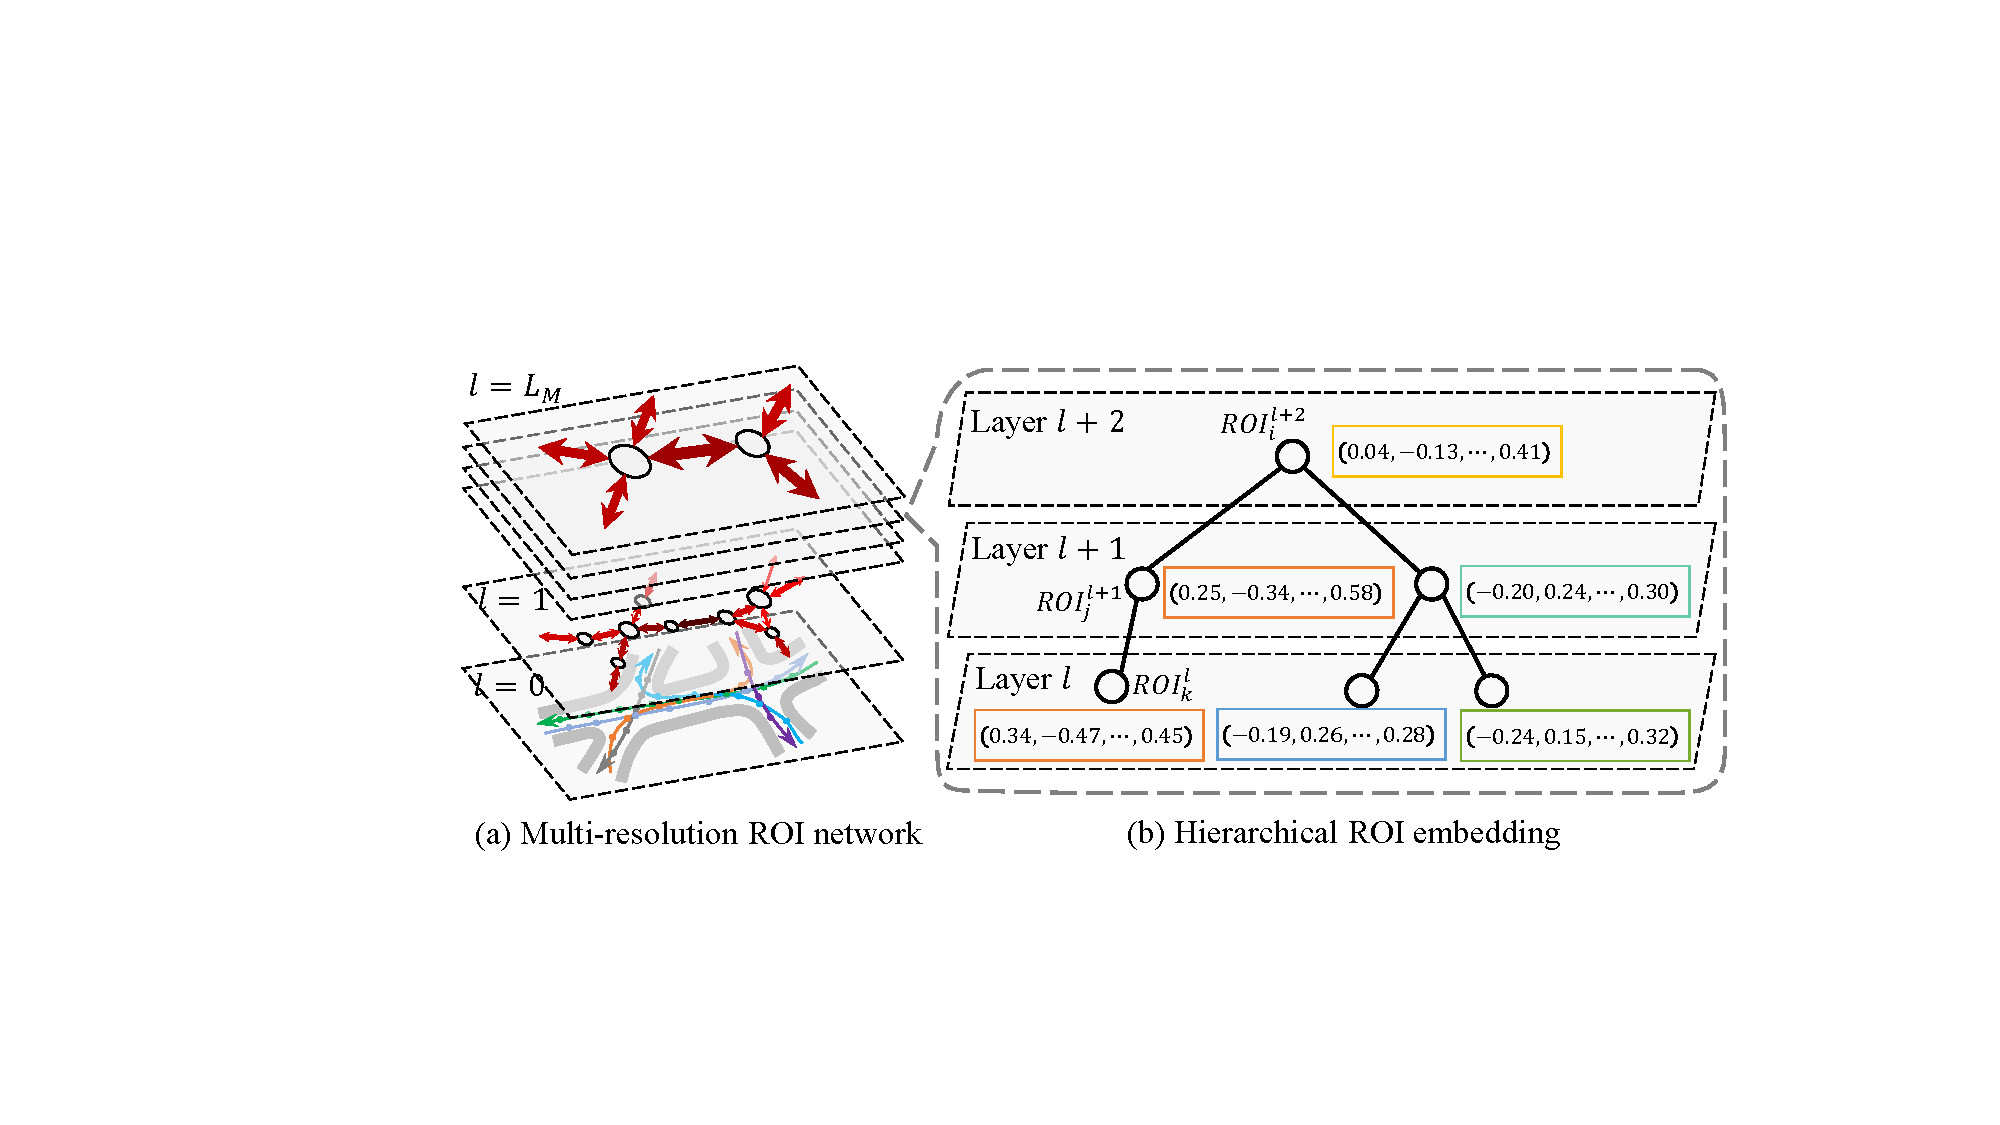
\includegraphics[width=130mm]{pics/Hembedding.pdf}
\caption {多层次语义ROI网络上的嵌入表征示意图。}
\label{fig:Hembedding}
\end{figure*}

模型的最大似然函数可写为:
\begin{equation}
\label{eq:optimizeFun}
L_{H^l} = \log\prod_{w\in{\mathcal{ROI}}^l}\prod_{u \in N(w)}{\hspace{-2mm}\sigma(\vec{t_w}\cdot{}\vec{s_u})}\hspace{-4mm}\prod_{v \in NEG(w)}{\hspace{-4mm}[1-\sigma(\vec{t_v}\cdot{}\vec{s_u})]}
\end{equation}
\begin{displaymath}
\hspace{2mm}= \hspace{-1mm}\sum_{\hspace{-2mm}w\in{\mathcal{ROI}}^l}\hspace{-2mm}\sum_{\hspace{2mm}u \in N(w)}\hspace{-1mm}\left\{{\hspace{-1mm}}\log\sigma(\vec{t_w}\cdot{}\vec{s_u})+ \hspace{-4mm}\sum_{v \in NEG(w)}{\hspace{-3mm}\log[1-\sigma(\vec{t_v}\cdot{}\vec{s_u})]}\right\}, \nonumber
\end{displaymath}

这个似然函数在嵌入空间中表示目标ROI的向量应该尽可能接近其邻域的所有矢量,同时区别其负样本的向量。

% \subsection{时间复杂度分析}
ROI嵌入模型的时间复杂度为$O(K \times N\times N_1\times N_2)$,其中$N$是点的数目,$N_1$是两种邻居的平均数量,$N_2$是负采样的样本个数,$K$是迭代的次数。

\subsection{多层次语义ROI网络的嵌入模型}

\smallsection{多层ROI网络不同层间的信息扩散}
嵌入过程在分层ROI网络的每一层上进行。此外,考虑到每个ROI都有父节点或子节点(除非它位于顶层或底层),我们做出一个直观的假设:每个ROI应该尽可能地在嵌入空间里与其父节点接近(如果存在)。 这种假设在显示中的语义下是合理的。例如,一个大商区的语义含义应包含位于该地区的公司或商店提供的所有功能。我们将这种信息传播写入嵌入模型的正则化项中:
\begin{equation}
\label{eq:optimizeFun2}
L_{V^l} = \sum_{w\in{\mathcal{ROI}^l}}\frac{1}{2}||\vec{t_w}-\vec{t_{\pi(w)}}||^2_2 + \frac{1}{2}||\vec{s_w}-\vec{s_{\pi(w)}}||^2_2,
\end{equation}
其中$\pi(w)$是ROI$w$的父节点。事实上父子节点间的影响可由在他们各自的向量上的约束来表示。图\ref{fig:Hembedding}(b)给出了一个例子,其中${ROI}_j^{l+1}$是第$l+1$层的一个ROI,它的向量被其父节点${ROI}_i^{l+2}$的向量和其子节点的${ROI}_k^{l}$的向量所约束。



最后,我们将原始的嵌入模型(\ref{eq:optimizeFun})以及约束项(\ref{eq:optimizeFun2})结合起来,得到了最后的目标方程:
\begin{equation}
\label{eq:optimizeFunAll}
\max \sum_{l=1:L_M} L_{H^l} - \alpha\hspace{-2mm}\sum_{l=1:L_M-1}\hspace{-2mm}L_{V^l}
\end{equation}
其中$\alpha$是一个折中系数。上面这个优化式可由随机梯度下降法(Stochastic Gradient Descent, SGD)来进行优化求解。参数的梯度项写在了算法\ref{alg:embedding}的7-17行里。



\subsection{轨迹的语义嵌入模型}
当我们得到所有ROI的嵌入向量后,我们可用ROI的权值加权求和得到轨迹的嵌入向量。给定一条轨迹$T^l = \{{ROI}^l_1, {ROI}^l_2, \cdots, {ROI}^l_n\}$在第$l$层上的表示。轨迹$T$最终的嵌入向量$\text{vec}(T)$可以表示为:
\begin{equation}
\label{eq:traVector}
\text{vec}(T) = \sum_{l=1}^{L_M}\sum_{i=1}^n\tau^l_i\cdot\text{vec}({ROI}^l_i),
\end{equation}
其中$\tau_i^l$是${ROI}^l_i$的权值,代表了轨迹$T$停留在${ROI}^l_i$的时间。注意这里也可以用更复杂的测量来求的轨迹的嵌入向量,比如加入衰减函数等。

值得注意的是,虽然这种获得轨迹向量的方式比起其他复杂的方法\citeup{socher2011dynamic,kalchbrenner2014convolutional,tai2015improved}要简单得多,但是简单的加权模型也非常的有效\citeup{blacoe2012comparison}。Wieting等人 \citeup{wieting2015towards}甚至证明了简单的加权模型性能要比复杂的神经网络要更好。再者,简单加权也是符合常识的:轨迹总是由采样点构成的。


\begin{algorithm}[!t]
\caption{语义轨迹嵌入模型}
\label{alg:embedding}
\SetKwData{True}{True}
\SetKwData{False}{False}
\SetKwFunction{Norm}{Norm}
\SetKwFunction{Count}{Count}
\SetKwFunction{Map}{Map}
\SetKwFunction{Length}{Length}
\SetKwFunction{Reduce}{Reduce}
\SetKwFunction{AverageKnn}{AverageKnn}
\SetKwFunction{RandomlyInit}{RandomlyInit}
\SetKwInOut{Input}{Input}
\SetKwInOut{Output}{Output}
\SetKwInOut{Parameter}{Parameter}
{
\Input{多层次ROI网络$G(V,E)$; ROI$w$的几何邻居和语义邻居$N(w)$;}
\Output{语义向量:vec$(ROI)$ 和 vec$(T)$;}
\Parameter{迭代次数$K$;学习率 $\eta$;折中系数$\alpha$;}
% \Parameter{Interaction range ${\epsilon}_0$; Incremental change $\triangle\epsilon$; Maximal layer $\mathcal{L}_M$; Learning rate $\eta$;}
\BlankLine

\lForEach {${ROI}^l_i\in{\mathcal{{ROI}}^l}$}{\RandomlyInit$(\vec{s_i}, \vec{t_i})$}
\ForEach {\emph{迭代数} $k \in \{1,2,\cdots,K\}$}{
\ForEach {\emph{层} $l \in \{1,2,\cdots,L_M-1\}$}{
% \ForEach {\emph{trajectory} $T^l=\{{ROI}^l_1,\cdots,{ROI}^l_{n^l}\}\in\mathcal{T}^l$}{
\ForEach {\emph{ROI网络上的节点} $w \in \mathcal{ROI}^l$}{
找寻$w$的两种邻居$N(w)$\;
对$w$进行负采样$NEG(w)$\;
\ForEach {$u \in N(w)$}{
$e = 0$\;
\ForEach {$v \in \{w\}\bigcup{}NEG(w)$}{
\lIf{$v == w$} {$I(v) = 1$; \textbf{else} $I(v) = 0$}
$g = \eta(I(v) - \sigma(\vec{t_v}\cdot\vec{s_u}))$;
$\vec{e} = \vec{e} + g\vec{t_v}$\;
$\vec{t_v} = \vec{t_v} + g\vec{s_u} + \eta\alpha(\vec{t_{\pi(v)}}-\vec{t_v})$\; %//update neighbors.\\ 
$\vec{t_{\pi(v)}} = \vec{t_{\pi(v)}} + \eta\alpha(\vec{t_v} - \vec{t_{\pi(v)}})$\; %//update neighbors' parent.\\
}
$\vec{s_u} = \vec{s_u} + \vec{e} + \eta\alpha(\vec{s_{\pi(u)}} - \vec{s_u})$\; %//update this ROI.\\
$\vec{s_{\pi(u)}} = \vec{s_{\pi(u)}} + \eta\alpha(\vec{s_{u}} - \vec{s_{\pi(u)}})$\; %//update parent.\\
}
}
% }
}
}
\lForEach {${ROI}_i \in \mathcal{ROI}$}{
vec$({ROI}_i) =[\vec{s_i}, \vec{t_i}]$
}
\lForEach {\emph{轨迹} $T\in\mathcal{T}$}{用式(\ref{eq:traVector})计算 $vec(T)$ }
% \ForEach {trajectory $T=\{{ROI}_1,{ROI}_2,\cdots,{ROI}_n\}\in\mathcal{T}$}{
% vec$(T) =\sum_i{\text{vec}(ROI}_i)$; //Obtain the trajectory vector \\
% }
}
\end{algorithm}

\subsection{ROI和轨迹的语义检索}
现实中,由于许多语义模式隐含在轨迹中,查询不能直接进行。作为替代方案,我们可以查询与选中地点或轨迹的最相似的位置或轨迹。也就是说,我们可以检索某个样本最相似的ROI或者轨迹,而不是直接构建复杂查询。

由于ROI或者轨迹在具有语义的连续空间中表示为向量,因此我们可以通过计算向量之间的距离来检索最相似的ROI或者轨迹。不失一般性,我们在这项工作中使用向量间的欧氏距离。




\section{实验设计}
\subsection{实验设置}

\smallsection{人工数据集}
和上一章节一样的方法,我们用概率路径规划算法\citeup{kavraki1996probabilistic}生成50条随机轨迹。我们随机选择10个点作为关键节点,并确保每个关键节点至少有一条轨迹通过。 语义ROI和轨迹检索任务旨在检测与这些关键点高度相关的ROI和轨迹。

\smallsection{真实数据集}
在上一章节Geolife和T-Drive轨迹数据的基础上,我们又引进了Kaggle 和Chengdu两个新的轨迹集。它们的统计信息在表\ref{tab:datasets}中。


% \tabcolsep=1pt
\begin{table}[!htb]\renewcommand{\arraystretch}{1.3}
% \vspace{-5mm}
\caption{四个真实数据集的统计信息}
% \vspace{-3mm}
\center
\small
\begin{tabular}{lcccc}
\hlinew{1pt} \textbf{Dataset}& \textbf{\#Point}& \textbf{\#Traj.}& \textbf{[Longitude, Latitude range]} & \textbf{[Width$\times$Height](m)}\\ \hlinew{1pt}
Geolife
& 24,876,978 & 18,670 & $[116.194, 116.553, 39.751, 40.033]$ & [31,024 $\times$ 31,368] \\
T-Drive
& 6,969,481 & 8,768 & $[116.194, 116.553, 39.751, 40.033]$ & [31,024 $\times$ 31,368] \\
Kaggle
& 78,239,735 & 1,704,769 & $[-8.702, -8.549, 41.135, 41.246]$ & [12,613$\times$ 12,365] \\
Chengdu
& 9,671,104 & 2,003 & $[103.913 ,104.180, 30.538, 30.765]$ & [25,484 $\times$ 25,219] \\
\hlinew{1pt}
\end{tabular}
\label{tab:datasets}
\end{table}

\smallsection{真实数据的区域语义获取方法}现实世界的轨迹数据富含各种语义信息,然而,真实的语义信息却通常很难获得。幸运的是,受益于在线地图服务的反向地理编码功能,比如MapBox API\footnote{\url{https://www.mapbox.com/}}和高德地图API\footnote{\url{https://www.amap.com /}},我们可以得到区域信息作为真实标签。具体而言,API可以将GPS坐标输入得到该地方的功能,例如银行,学校或市场。因此,我们将每个ROI的语义真实语义标签定义为其功能类别的分布,并将两个ROI$A$和$B$的真实相似性定义为两个分布的相交部分:
\begin{equation}
\mathrm{Sim}(A,B) = \sum{\min\left(\text{distribution}(A),{\text{distribution}(B)}\right)}.
\label{eq:SIM}
\end{equation}
举一个例子,若$A$点的功能分布为: \{银行,学校,市场,音乐\} = $\{0.2, 0.7, 0.1, 0\}$,而$B$点的为:\{银行,学校,市场,音乐\} = $\{0.4, 0.3, 0, 0.3\}$。那么两个点的相似度则可写为$\mathrm{Sim}(A,B) = 0.2 + 0.3 + 0 + 0 = 0.5$。这种定义方式是直观的。

\smallsection{真实数据的轨迹语义获取方法} 
类似的,通过分别利用以上所述的API和式(\ref{eq:SIM}),我们使用一种直观的方法来获取轨迹的真实语义分布。由于轨迹由一组采样点组成,因此该轨迹的真实语义标签可以通过其采样点的真实语义标签的归一化和来表示。此外,由于原始GPS点太多,调用地图API太繁杂。因此我们使用\CascadeSync算法对原始GPS进行处理得到一个单层ROI网络,取交互参数$\epsilon = 1/200 *(w + h)$,其中$ w,h $是地图的宽度和高度。用这种方式将数百万的GPS点数减少到数千个ROI。就容易地获得真实语义标签和相似性。注意我们后面也会用到这个辅助ROI网络。

对于语义轨迹检索,如果检索到的轨迹与查询轨迹重叠,即它们与查询轨迹共享大多数ROI,则NDCG@k值将是完美的。然而,这种类型的轨迹是不需要的,因此,我们规定当且仅当一条检索出的轨迹与辅助ROI网络上的被查询的轨迹共享小于$50\%$的ROI时,检索的轨迹才是有效的。


\tabcolsep=1pt
\begin{figure}[!t]
\centering
% \footnotesize
\begin{tabular}{ccc}
\includegraphics[width=48mm]{pics/syn1.eps}&
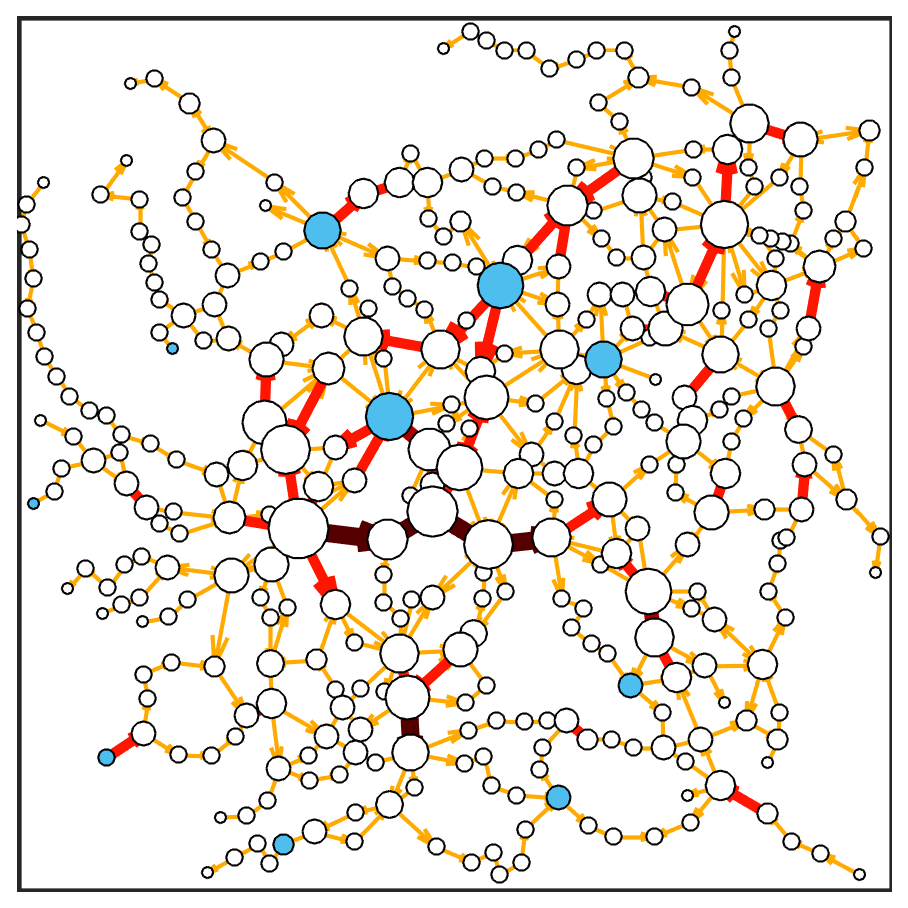
\includegraphics[width=48mm]{pics/syn2.eps}&
\includegraphics[width=48mm]{pics/syn3.eps}\\
(a) & (b) & (c) \\
\end{tabular}
% \vspace{-4mm}
\caption{
人工数据集和结果的示意图。(a)关键点和原始轨迹数据。10个五边形是随机生成的关键点。(b)多层次ROI网络的底层。蓝色ROI是关键ROI,其至少包含一个关键点。(c)轨迹检索结果。黑色轨迹是目标。检索结果为不同色调的绿色轨迹。颜色越深,与目标越相似,即包含更多关键ROI。}
\label{fig:syn}
% \vspace{-3mm}
\end{figure}


\smallsection{评价指标}
为了衡量语义检索结果的准确性,我们需要定义ROI和轨迹的真实目标。在人工实验中,真的关键节点隐含在10个关键点里。对于相似ROI检索任务,给定任何关键点,最相似的ROI应该是包含其他九个关键点的ROI,这些关键点被称为真实ROI。检索性能通过正确检测到的真实ROI的比率来衡量。对于轨迹检索任务,我们选择目标轨迹作为尽可能多地通过真实ROI。在这种情况中,目标轨迹应该包含尽可能多的真实ROI。因此,我们可以获得检索到的轨迹并进行排序,然后比较真实顺序和检索顺序来计算累计收益(NDCG@k),其定义如下。

接下来,我们可以执行ROI或者轨迹的语义检索了,并计算检索结果的ROI或者轨迹和真实ROI或轨迹之间的NDCG@k度量。此外,我们可以将算法的性能与国际最主流的相似性算法DTW,LCSS,EDR和Fr\'echet距离进行比较。在不失一般性的情况下,我们也在上述辅助ROI网络上计算这四个比较度量。
\begin{equation}
\mathrm{NDCG@k} = \frac{\mathrm{DCG@k}}{\mathrm{IDCG@k}},
\label{eq:NDCG}
\end{equation}
其中$\mathrm{IDCG@k}$是$\mathrm{DCG@k}$的理想取值,而$\mathrm{DCG@k}$定义如下:
\begin{equation}
\mathrm{DCG@{k}} = \sum_{i=1}^{k} \frac{ 2^{rel_{i}} - 1 }{ \log_{2}(i+1)},
\label{eq:DCG}
\end{equation}
其中$rel_i$是位置$i$处的相关度。为了试验更加清晰,我们采用5个级别的相关度。

\tabcolsep=0.5pt
% \vspace{-4mm}
\begin{figure}[!b]
% \vspace{-3mm}
\centering
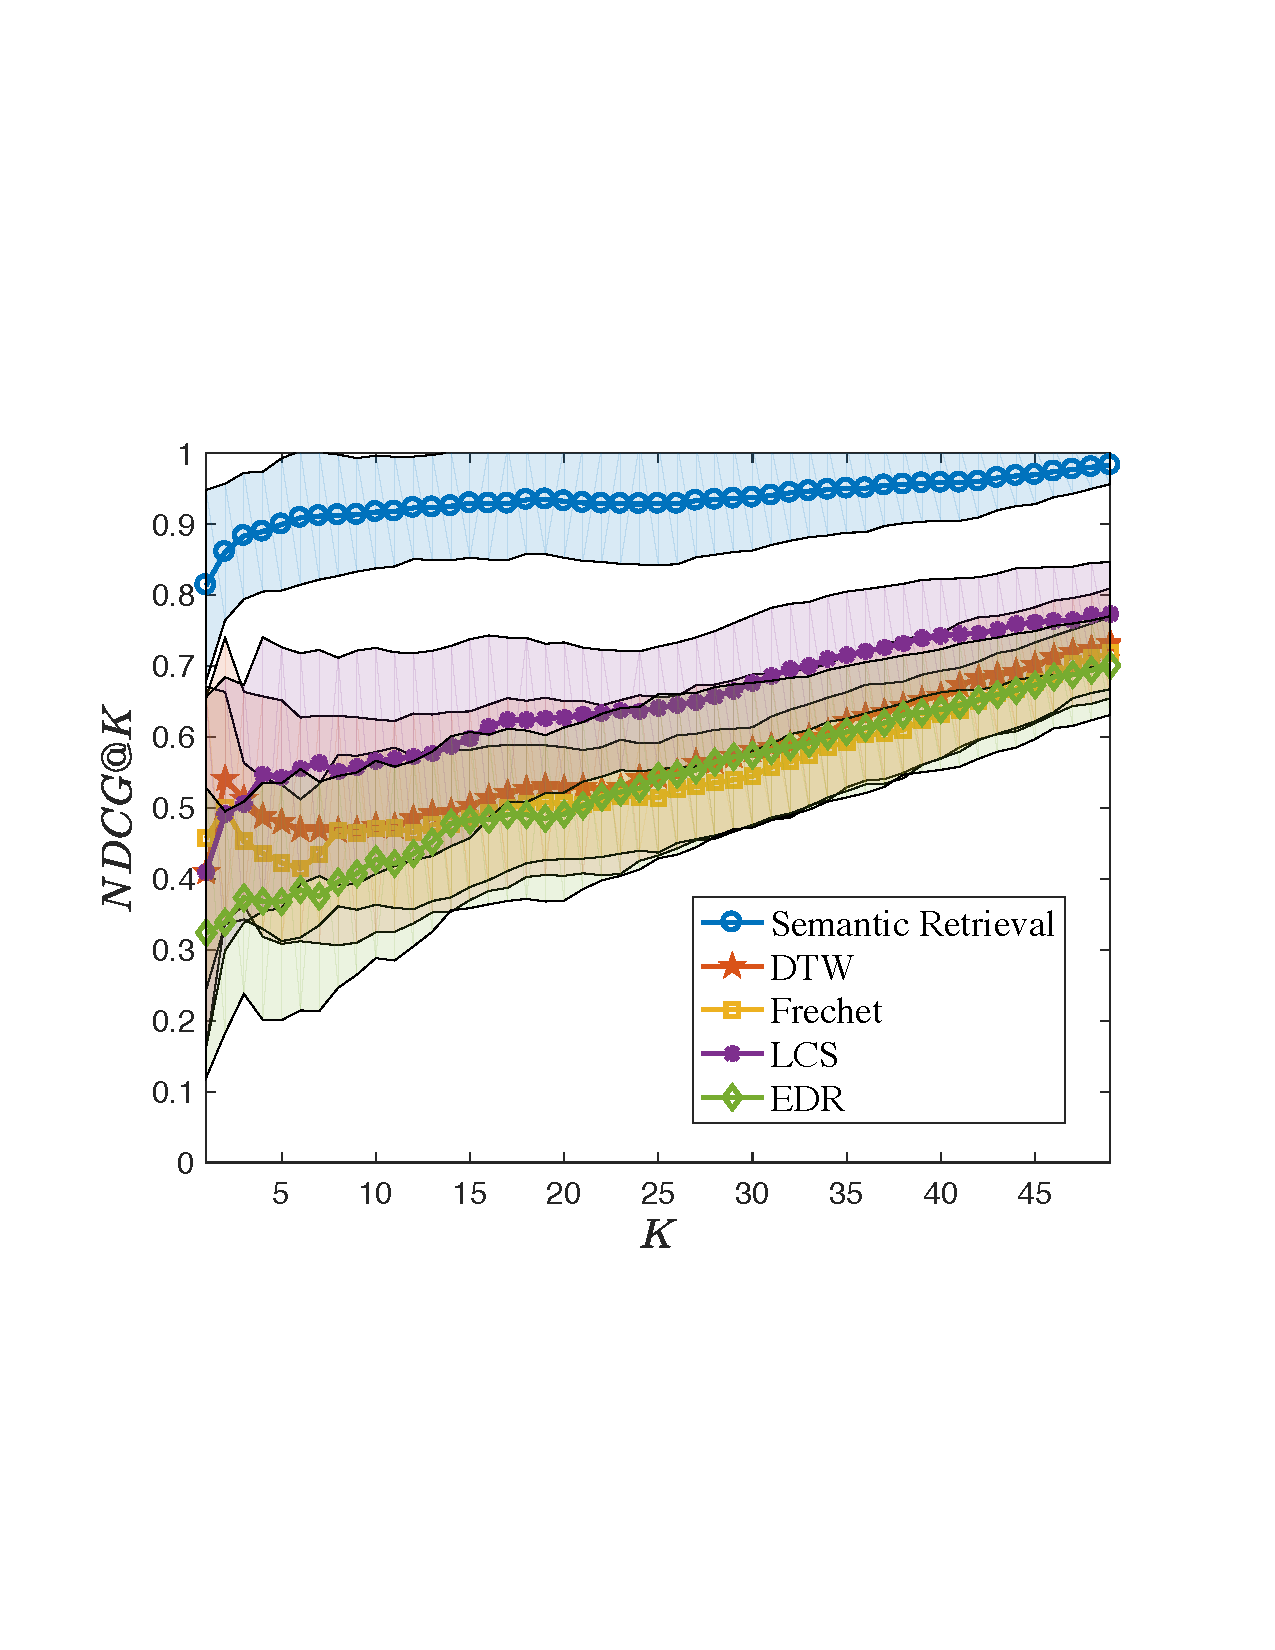
\includegraphics[width=100mm]{pics/synNDCG.pdf}
% \vspace{-4mm}
\caption{人工数据集上的语义轨迹检索结果。阴影部分是100次检索的标准差区域。}
\label{fig:synNDCG}
\end{figure}


\subsection{实验结果与分析}
% \subsection{人工数据集上的验证}
在人工数据集上设定交互范围 $\epsilon = \{2,4,6,8,10\}(m)$,运用\CascadeSync算法后得到一个5层的ROI网络。最下面的一层可视化在图\ref{fig:syn}(b)中。


\smallsection{人工数据集上的关键节点检测结果}
在此任务中,我们使用领域知识:ROI是否包含任何关键点。为了测试这些关键ROI是否具有相似的向量表征,我们评估了给定关键ROI的最相似ROI的检索准确性(图\ref{fig:syn}(b)中的蓝色ROI)。 理想的检索结果是所有关键ROI都比那些非关键ROI更相似。

在ROI和轨迹的嵌入向量的基础上,我们搜索最相似的ROI。实验在随机生成的数据集上独立重复100次。得到的平均准确度为$\boldsymbol{99.64\%}$,这证明了关键点的语义成功地整合到嵌入表示中,并且可以有效地检测到关键点。



\tabcolsep=2pt
\begin{figure}[!t]
\centering
% \vspace{-2mm}
% \footnotesize
\begin{tabular}{cc}
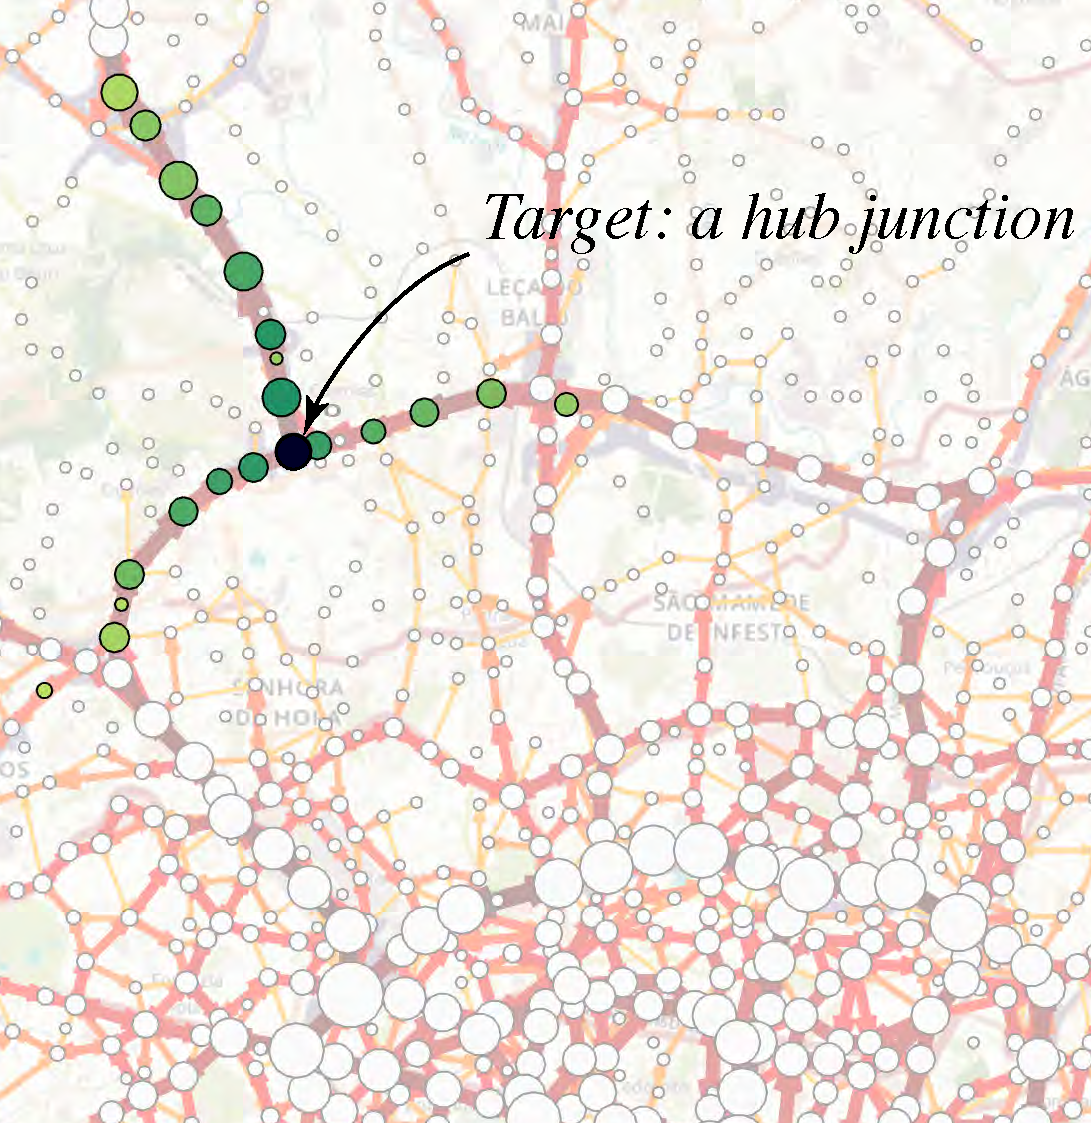
\includegraphics[width=65mm]{pics/SP3.pdf}&
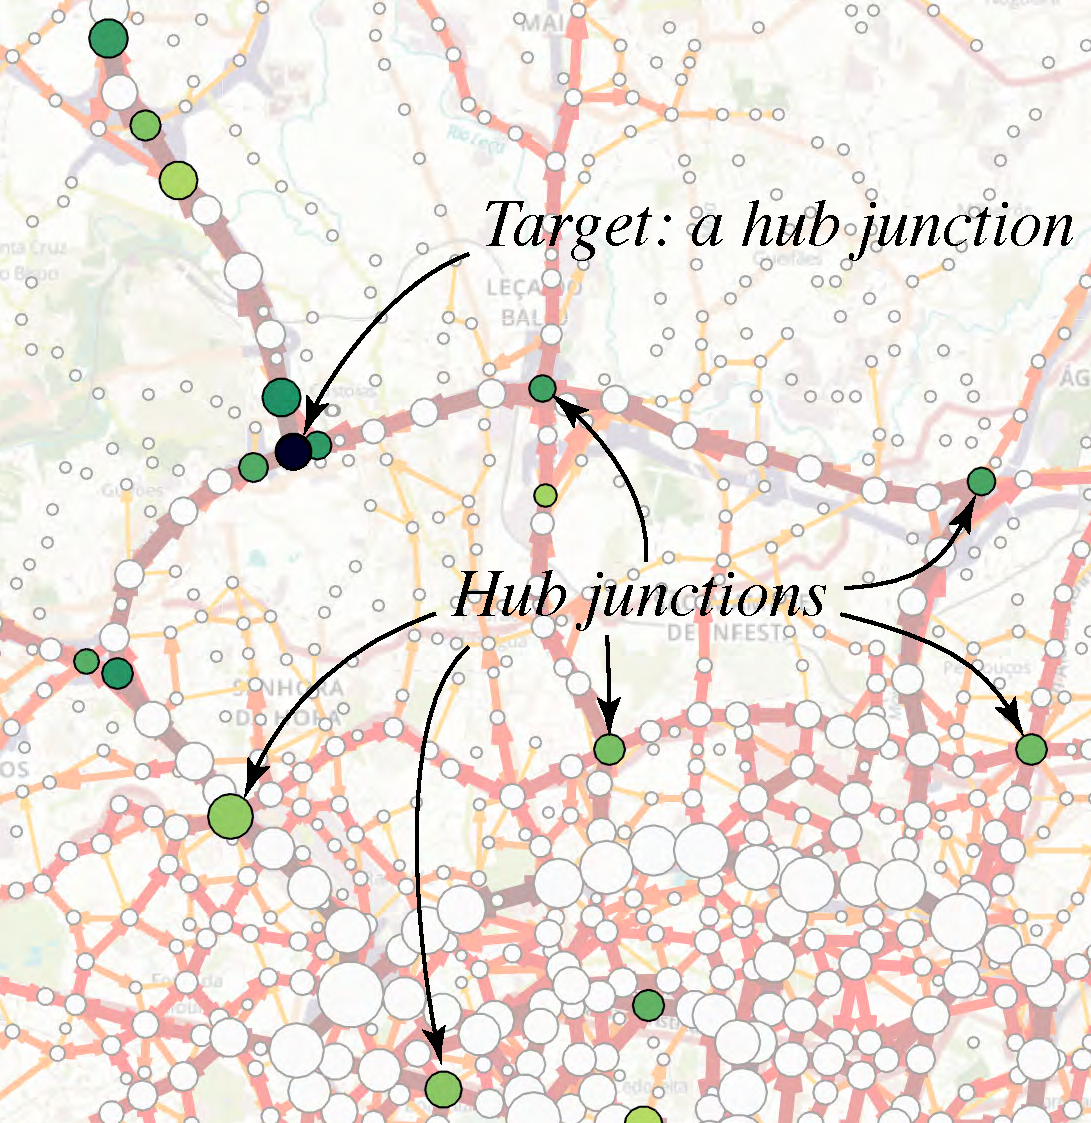
\includegraphics[width=65mm]{pics/SP4.pdf}\\
(a) 没有语义信息 & (b) 有语义信息
% \multicolumn{2}{c}{(a) Geolife} & & \multicolumn{2}{c}{(b) Kaggle Taxi}\\
\end{tabular}
% \vspace{-2mm}
\caption{在Kaggle数据集上的相似ROI检索结果。}
% \vspace{-2mm}
\label{fig:regionSim}
\end{figure}

\smallsection{人工数据集上的语义轨迹检测结果。}
我们在轨迹层面上进行类似的实验,目的是检索与包含最多关键ROI相似的目标轨迹,因此类似的轨迹应包含尽可能多的关键ROI。我们计算并确定其余49个轨迹与目标的相似度,并使用NDCG@k,即式(\ref{eq:NDCG})来给定排名。在图\ref{fig:syn}(c)中我们可视化了最相似的轨迹,其中绿色轨迹的颜色深浅与检索顺序成正比。此外,我们使用第一层ROI网络(具有关键ROI标签的最佳级别)上的四个对比算法进行相同的实验。结果如图\ref{fig:synNDCG}所示。实验重复100次,阴影部分给出平均NDCG@k值的标准偏差。从图中可以看出,我们的模型优于其他四个模型,很好地捕获了语义信息。




\smallsection{真实数据集上的检索结果}

实验的目标为给定一个ROI,检索前5个最相似的ROI,并计算NCDG@5。此外,给定一条轨迹,我们检索前10个最相似的轨迹,计算NCDG@3,5,10,并与对比算法进行比较。此外,我们将每个ROI邻居的数量设置为3,将负抽样的样本数设置为5,并交互范围设置为$\epsilon(l) = l \times 1/200\times(width + height), l = \{1,\cdots,5\}$来产生一个5层的ROI网络。

为了探索不同语义信息对现实数据检索性能的影响,我们取三种不同累心的模型来做实验:1)仅几何信息(即基本轨迹结构)。2)几何和基本语义(即网络特征和时间信息)。3)所有类型的邻居和领域知识。此外,我们通过构建两个嵌入模型来研究特征传播的效果:仅在ROI网络的底层($\epsilon(t) = 1/200 \times(width + height)$)用公式(\ref{eq:optimizeFun})进行训练,以及在ROI网络的5个层用式(\ref{eq:optimizeFunAll})进行训练。

为了更好地说明ROI检索的结果,我们选择Kaggle数据集中的一个枢纽十字路口作为目标ROI。我们在上述5层网络中运用了具有和不具有语义邻居的嵌入模型,检索结果如图\ref{fig:regionSim}所示。从结果来看,具有语义邻居的模型可以捕获语义信息,从而容易地识别区域的功能,并且能够检索到远离查询目标十字路口的其他枢纽十字路口。原因在于交通的语义可以通过节点度以及度分布的信息在ROI网络上反映出来,因此不会受到几何位置的限制。

ROI检索和轨迹检索的结果分别列在表\ref{tab:ROIEvaluation}和表\ref{tab:Evaluation_trajectory}中。从表中我们有三个发现:(1)嵌入模型中考虑的语义邻居越多,嵌入模型的性能越好;(2)当没有领域知识可用时,分层ROI网络上的嵌入模型优于单层模型的结果,这意味着分层结构通过特征传播促进了嵌入向量的表征能力。(3)当嵌入模型中融入领域知识后,性能主要依赖于领域知识的标签质量。


\tabcolsep=3pt
\begin{table}[tbh!]\renewcommand{\arraystretch}{1.3}
\caption{ROI检索在NDCG@5指标上的结果。模型1仅考虑几何邻居。模型2考虑了几何邻居和基本的语义信息。模型3考虑了真实的标签信息。}
% \vspace{-2mm}
\center
\small
\begin{tabular}{cccccc}
\hlinew{1pt}
\textbf{数据集} &\textbf{结构} & \textbf{Random} & \textbf{模型1} & \textbf{模型2}&\textbf{模型3} \\[0.4ex] \hlinew{0.85pt}
%Colon
\multirow{2}{*}{Geolife} & One-layer & \multirow{2}{*}{0.429 $\pm$ 0.24} & 0.526 $\pm$ 0.18 & 0.560 $\pm$ 0.15 & 0.713 $\pm$ 0.18\\
&Hierarchical & & 0.581 $\pm$ 0.15 & 0.615 $\pm$ 0.13 & \textbf{0.724 $\pm$ 0.17}\\
\hline
\multirow{2}{*}{T-Drive} & One-layer & \multirow{2}{*}{0.382 $\pm$ 0.23} & 0.592 $\pm$ 0.21 & 0.521 $\pm$ 0.18 & \textbf{0.713 $\pm$ 0.21}\\
&Hierarchical & & 0.650 $\pm$ 0.24 & 0.655 $\pm$ 0.23 & 0.693 $\pm$ 0.18\\
\hline
\multirow{2}{*}{Kaggle} & One-layer & \multirow{2}{*}{0.410 $\pm$ 0.28} & 0.524 $\pm$ 0.20 & 0.542 $\pm$ 0.22 & 0.679 $\pm$ 0.19\\
&Hierarchical & & 0.524 $\pm$ 0.22 & 0.567 $\pm$ 0.21 & \textbf{0.691 $\pm$ 0.16}\\
\hline
\multirow{2}{*}{Chengdu} & One-layer & \multirow{2}{*}{0.415 $\pm$ 0.25} & 0.666 $\pm$ 0.20 & 0.677 $\pm$ 0.21 & \textbf{0.817 $\pm$ 0.17}\\
&Hierarchical & & 0.697 $\pm$ 0.23 & 0.665 $\pm$ 0.20 & 0.802 $\pm$ 0.16\\
\hlinew{1pt}
\end{tabular}
\label{tab:ROIEvaluation}
\end{table}



\begin{table*}[tbh!]\renewcommand{\arraystretch}{1.3}
\caption{四个真实数据集上的轨迹语义检索。}
% \vspace{1mm}
\center
\small
\tabcolsep=2pt
\begin{tabular}{ccccccc}
\hlinew{1pt}
\textbf{数据集} & \textbf{指标} & \textbf{Random} & \textbf{DTW} & \textbf{Frechet} & \textbf{LCSS} & \textbf{EDR}\\
\hlinew{0.85pt}

\multirow{3}{*}{\textbf{Geolife}} 
&NDCG@3 &0.254 $\pm$ 0.158 & 0.391 $\pm$ 0.198 & 0.328$ \pm $0.179 & 0.360 $\pm$ 0.258 & 0.340 $\pm$ 0.189   \\
&NDCG@5 &0.272 $\pm$ 0.130 & 0.410 $\pm$ 0.185 & 0.393$ \pm $0.178 & 0.368 $\pm$ 0.224 & 0.411 $\pm$ 0.171   \\
&NDCG@10 &0.293 $\pm$ 0.127 & 0.521 $\pm$ 0.134 & 0.439$ \pm $0.165 & 0.379 $\pm$ 0.184 & 0.467 $\pm$ 0.171 \\
\hline
\multirow{3}{*}{\textbf{T-Drive}} 
&NDCG@3 &0.286 $\pm$ 0.182 & 0.416 $\pm$ 0.201 & 0.304$ \pm $0.191 & 0.396 $\pm$ 0.241 & 0.358 $\pm$ 0.195   \\
&NDCG@5 &0.290 $\pm$ 0.172 & 0.430 $\pm$ 0.168 & 0.346$ \pm $0.156 & 0.402 $\pm$ 0.211 & 0.363 $\pm$ 0.184   \\
&NDCG@10 &0.343 $\pm$ 0.169 & 0.443 $\pm$ 0.149 & 0.371$ \pm $0.141 & 0.402 $\pm$ 0.180 & 0.379 $\pm$ 0.161 \\
\hline
\multirow{3}{*}{\textbf{Kaggle}} 
&NDCG@3 &0.255 $\pm$ 0.220 & 0.311 $\pm$ 0.223 & 0.250$ \pm $0.175 & 0.349 $\pm$ 0.227 & 0.290 $\pm$ 0.182   \\
&NDCG@5 &0.276 $\pm$ 0.225 & 0.321 $\pm$ 0.215 & 0.288$ \pm $0.151 & 0.375 $\pm$ 0.218 & 0.304 $\pm$ 0.177   \\
&NDCG@10 &0.307 $\pm$ 0.201 & 0.342 $\pm$ 0.207 & 0.300$ \pm $0.148 & 0.382 $\pm$ 0.214 & 0.308 $\pm$ 0.162 \\
\hline
\multirow{3}{*}{\textbf{Chengdu}} 
&NDCG@3 &0.303 $\pm$ 0.210 & 0.417 $\pm$ 0.168 & 0.360$ \pm $0.239 & 0.314 $\pm$ 0.241 & 0.416 $\pm$ 0.196   \\
&NDCG@5 &0.320 $\pm$ 0.208 & 0.442 $\pm$ 0.153 & 0.388$ \pm $0.229 & 0.346 $\pm$ 0.221 & 0.424 $\pm$ 0.171   \\
&NDCG@10 &0.345 $\pm$ 0.205 & 0.457 $\pm$ 0.145 & 0.417$ \pm $0.211 & 0.376 $\pm$ 0.209 & 0.449 $\pm$ 0.179 \\
% \hlinew{1pt}
\end{tabular}

\tabcolsep=7pt
\begin{tabular}{ccccccc}
\hlinew{1pt}
\multirow{2}{*}{\textbf{数据集}} & \multirow{2}{*}{\textbf{指标}} & \multicolumn{2}{c}{\textbf{单层模型}} & \multicolumn{2}{c}{\textbf{多层模型}}\\
\cline{3-6}
&& \textbf{无领域知识} & \textbf{有领域知识} & \textbf{无领域知识} & \textbf{有领域知识}\\
\hlinew{0.85pt}

\multirow{3}{*}{\textbf{Geolife}} 
&NDCG@3 & 0.468 $\pm$ 0.177 & 0.607 $\pm$ 0.152 & 0.545 $\pm$ 0.171 & \textbf{0.663 $\pm$ 0.148} \\
&NDCG@5 & 0.483 $\pm$ 0.165 & 0.639 $\pm$ 0.120 & 0.552 $\pm$ 0.162 & \textbf{0.676 $\pm$ 0.104} \\
&NDCG@10& 0.520 $\pm$ 0.156 & 0.657 $\pm$ 0.109 & 0.558 $\pm$ 0.148 & \textbf{0.689 $\pm$ 0.094}\\
\hline
\multirow{3}{*}{\textbf{T-Drive}}
&NDCG@3 & 0.529 $\pm$ 0.169 & 0.697 $\pm$ 0.179 & 0.547 $\pm$ 0.182 & \textbf{0.717 $\pm$ 0.184} \\
&NDCG@5 & 0.545 $\pm$ 0.144 & \textbf{0.711 $\pm$ 0.172} & 0.564 $\pm$ 0.169 & 0.702 $\pm$ 0.183 \\
&NDCG@10& 0.544 $\pm$ 0.139 & \textbf{0.734 $\pm$ 0.168} & 0.599 $\pm$ 0.155 & 0.721 $\pm$ 0.175\\
\hline
\multirow{3}{*}{\textbf{Kaggle}}
&NDCG@3 & 0.406 $\pm$ 0.185 & 0.593 $\pm$ 0.164 & 0.438 $\pm$ 0.183 & \textbf{0.600 $\pm$ 0.209}\\
&NDCG@5 & 0.413 $\pm$ 0.160 & \textbf{0.604 $\pm$ 0.150} & 0.445 $\pm$ 0.151 & 0.602 $\pm$ 0.183\\
&NDCG@10& 0.430 $\pm$ 0.150 & 0.607 $\pm$ 0.157 & 0.452 $\pm$ 0.145 & \textbf{0.626 $\pm $0.188}\\
\hline
\multirow{3}{*}{\textbf{Chengdu}}
&NDCG@3 & 0.588 $\pm$ 0.159 & 0.824 $\pm$ 0.143 & 0.611 $\pm$ 0.160 & \textbf{0.833 $\pm$ 0.120}\\
&NDCG@5 & 0.622 $\pm$ 0.124 & \textbf{0.859 $\pm$ 0.139} & 0.635 $\pm$ 0.139 & 0.849 $\pm$ 0.112\\
&NDCG@10& 0.651 $\pm$ 0.112 & \textbf{0.866 $\pm$ 0.113} & 0.666 $\pm$ 0.114 & 0.862 $\pm$ 0.096\\
\hlinew{1pt}
\end{tabular}
\label{tab:Evaluation_trajectory}
\end{table*}

\section{本章小结}
在本章中,我们提出了一种新的语义轨迹嵌入表征方法。首先,经过 \CascadeSync模型将原始轨迹先转换为多层次的ROI网络。在这个网络上,可以依靠几何,语义,时间等信息以及作为上下文找到嵌入模型中的两种类型的邻居,其次利用负采样算法,计算出每一层ROI和轨迹的分布式表征向量。得到这个向量后,课通过直接计算向量间的欧几里德距离来高效地执行语义检索任务。在人工数据集和现实数据集上,本文的方法有效地提取并表征了语义信息,效果超过了四种主流算法。

% \newpage\mbox{}\thispagestyle{empty}\newpage

% % !Mode:: "TeX:UTF-8"

\chapter{全文总结与展望}
\label{chapter:conclusion}
\section{全文总结}
本文我们介绍了目前比较火热的双边聚类问题,提出一种基于同步原理的全新的双边聚类算法\cosync,并在人工数据集以及基因数据集上进行测试,取得了优秀的成果。各章节的主要内容总结如下:

\begin{itemize}
  \item ~~第\ref{chapter:introduction}章为引言部分,从数据挖掘的聚类领域谈起,介绍了双边聚类需求的产生,并正式定义了双边问题以及联合簇。
  \item ~~第\ref{chapter:rw}章的第一部分整理和回顾了国际上相关的知名研究成果。介绍了从两个角度对联合簇具体形式的分类,之后对现有的大部分双边聚类算法进行了分类总结,将它们大致分为基于启发式搜索的方法和非度量式方法,针对每个方法都列举了一些算法的工作原理。接下来第二部分介绍了自然界中同步的概念以及用同步思想作为聚类原理的\sync算法。
  \item ~~第\ref{chapter:main}章开始正式介绍\cosync算法的多个步骤。以同步聚类思想为切入点,我们提出了全新的双边加权交互模型,使得数据集矩阵中的联合簇能够随着时间自动收敛为常数值。在交互模型收敛后,我们提出了一种启发式的同值子矩阵搜索算法来挖掘结果矩阵中的常数值子块。最后,为了能够处理高维数据,避开高维诅咒的困扰,我们引入非负矩阵分解。至此,\cosync算法便能在大规模数据矩阵中进行联合簇挖掘。
  \item ~~第\ref{chapter:experiment}章为实验部分,为了证明\cosync算法的可行性和高效性,我们将双边聚类中有代表性的ITCC,MSSRCC,Spectral Clustering和Plaid算法一起加入实验。实验在人工数据集和基因数据集上展开,最后结果显示\cosync具有极好的性能,超越了其他对比算法。
\end{itemize}


\section{后续工作展望}
本文中我们已经完成了关于双边聚类新算法\cosync的所有工作,之后我们将对全新的工作开展工作,即围绕\textbf{多边聚类}问题进行研究。

考虑这样一个问题,在推荐系统中,我们能得到不同用户在不同时间内,对不同商品的喜好数据,这种数据可以写为一个数据立方体$A$,其中任一元素$A_{ijk}$表示第$i$个用户在$k$个时间段内,对$j$个商品的评分。类比双边聚类,多边聚类即在类似的时间段内,找出相似的用户以及对应的相应的商品。

双边聚类的原理是在数据矩阵中,对每一个元素都用其行列邻居对它进行交互,最终达到同步的状态。那现在拓展这个思想,我们在一个数据立方体甚至更高维数据张量(tensor)\footnote{\url{https://en.wikipedia.org/wiki/Tensor}}中,仍然用这种同步交互的思想,对数据张量中的元素进行动态交互。图\ref{future}给出了在数据矩阵上进行双边聚类以及在数据立方体上进行多边聚类的交互示意图。

\pic[h]{从双边聚类到多边聚类}{}{future}

如图\ref{future}(b)所示,数据立方体中任一元素将被其$x,y,z$三个维度上的邻居影响交互,随着时间迭代最后达到同步的状态。此时的聚类簇结构将表现为数据立方体中包含的常数子块。

关于多边聚类问题,目前国际上研究的成果很少。一方面,真实世界中,不稀疏的数据立方体或者更高维的数据很难获取,另一方面,处理这样的数据困难而效率低下。我们将用同步的思想,对多边聚类问题展开研究,争取在这一领域作出成果,向国际研究前沿进军。路漫漫其修远兮,吾将上下而求索!



\end{document}



